%----------------------------------------------------------------------------------------
%	PACKAGES AND OTHER DOCUMENT CONFIGURATIONS
%----------------------------------------------------------------------------------------

\documentclass[a4paper, reqno]{book} 
                
% inputs the file which contains all the document configurations and packages - make sure to edit this file
%----------------------------------------------------------------------------------------
%	DOCUMENT VARIABLES
%	Fill in the lines below to enter your information into the thesis template
%	Each of the commands can be cited anywhere in the thesis
%----------------------------------------------------------------------------------------

\newcommand{\myTitle}{Smart gateway for Low-Power Lossy Networks\xspace}
\newcommand{\mySubtitle}{A PhD thesis\xspace}
\DeclareRobustCommand{\myName}{Remy Leone\xspace}

\newcommand{\Paolo}{Dr. Paolo MEDAGLIANI\xspace}
\newcommand{\Jeremie}{Dr. Jeremie LEGUAY\xspace}
\newcommand{\Claude}{Dr. Claude CHAUDET\xspace}
\newcommand{\Vania}{Dr. Vania CONAN\xspace}
\newcommand{\JeanLouis}{Dr. Jean Louis ROUGIER\xspace}

\newcommand{\myFaculty}{INFRES\xspace}
\newcommand{\myDepartment}{Network and Computer Science Department\xspace}
\newcommand{\myUni}{Telecom Paris Tech\xspace}
\newcommand{\myLocation}{Paris, France\xspace}
\newcommand{\myTime}{\today\xspace}

%----------------------------------------------------------------------------------------
%	USEFUL COMMANDS
%----------------------------------------------------------------------------------------

\newcommand{\ie}{i.\,e.}
\newcommand{\Ie}{I.\,e.}
\newcommand{\eg}{e.\,g.}
\newcommand{\Eg}{E.\,g.} 

\newcounter{dummy} % Necessary for correct hyperlinks (to index, bib, etc.)
% \providecommand{\mLyX}{L\kern-.1667em\lower.25em\hbox{Y}\kern-.125emX\@}

%----------------------------------------------------------------------------------------
%	PACKAGES
%----------------------------------------------------------------------------------------

%\usepackage[francais]{babel}
\usepackage{lipsum} % Used for inserting dummy 'Lorem ipsum' text into the template 
\usepackage[utf8]{inputenc} 
\usepackage[fleqn]{amsmath} % Math environments and more by the AMS 
\usepackage{xspace} % To get the spacing after macros right
\usepackage{mparhack} % To get marginpar right
\usepackage{fixltx2e} % Fixes some LaTeX stuff 

\PassOptionsToPackage{smaller}{acronym} % Include printonlyused in the first bracket to only show acronyms used in the text
\usepackage{acronym} % nice macros for handling all acronyms in the thesis

%------------------------------------------------

%\renewcommand*{\acsfont}[1]{\textssc{#1}} % For MinionPro
\renewcommand{\bflabel}[1]{{#1}\hfill} % Fix the list of acronyms


\usepackage[backend=biber,style=alphabetic,sorting=ynt]{biblatex}
\addbibresource{main.bib}
\usepackage[pdftex]{graphicx} 

\usepackage[l2tabu, orthodox]{nag} % Static Analysis of LaTeX source code

%------------------------------------------------
% Telecom Paris Tech
%------------------------------------------------

\usepackage{geometry}
\usepackage{eso-pic}
\usepackage{ifpdf}

\newcommand\BackgroundPicLastPage{
\ifpdf
	\includegraphics[height=\paperheight,width=\paperwidth]{img/logos/cover_4_bg.pdf}
\else
	\includegraphics[height=\paperheight,width=\paperwidth]{img/logos/cover_4_bg.pdf}
\fi
}

\newcommand\BackgroundPicCover{
\ifpdf
	\includegraphics[height=\paperheight,width=\paperwidth]{img/logos/cover_bg.pdf}
\else
	\includegraphics[height=\paperheight,width=\paperwidth]{img/logos/cover_bg.pdf}
\fi}

%----------------------------------------------------------------------------------------
%	FLOATS: TABLES, FIGURES AND CAPTIONS SETUP
%----------------------------------------------------------------------------------------

\usepackage{tabularx} % Better tables
\setlength{\extrarowheight}{3pt} % Increase table row height
\newcommand{\tableheadline}[1]{\multicolumn{1}{c}{\spacedlowsmallcaps{#1}}}
\newcommand{\myfloatalign}{\centering} % To be used with each float for alignment
\usepackage{caption}
\captionsetup{format=hang,font=small}
\usepackage{subfig}  

%----------------------------------------------------------------------------------------
%	CODE LISTINGS SETUP
%----------------------------------------------------------------------------------------

\usepackage{listings} 
%\lstset{emph={trueIndex,root},emphstyle=\color{BlueViolet}}%\underbar} % for special keywords
\lstset{language=[LaTeX]Tex, % Specify the language for listings here
% keywordstyle=\color{Blue}, % Add \bfseries for bold
basicstyle=\small\ttfamily, % Makes listings a smaller font size and a different font
%identifierstyle=\color{NavyBlue}, % Color of text inside brackets
commentstyle=\color{Green}\ttfamily, % Color of comments
stringstyle=\rmfamily, % Font type to use for strings
numbers=left, % Change left to none to remove line numbers
numberstyle=\scriptsize, % Font size of the line numbers
stepnumber=5, % Increment of line numbers
numbersep=8pt, % Distance of line numbers from code listing
showstringspaces=false, % Sets whether spaces in strings should appear underlined
breaklines=true, % Force the code to stay in the confines of the listing box
%frameround=ftff, % Uncomment for rounded frame
frame=single, % Frame border - none/leftline/topline/bottomline/lines/single/shadowbox/L
belowcaptionskip=.75\baselineskip % Space after the "Listing #: Desciption" text and the listing box
}

%----------------------------------------------------------------------------------------
%	HYPERREFERENCES
%----------------------------------------------------------------------------------------

\PassOptionsToPackage{pdftex,hyperfootnotes=false,pdfpagelabels}{hyperref}
\usepackage{hyperref}  % backref linktocpage pagebackref
\pdfcompresslevel=9
\pdfadjustspacing=1

\hypersetup{
% Uncomment the line below to remove all links (to references, figures, tables, etc)
%draft, 
colorlinks=true, linktocpage=true, pdfstartpage=3, pdfstartview=FitV,
% Uncomment the line below if you want to have black links (e.g. for printing black and white)
%colorlinks=false, linktocpage=false, pdfborder={0 0 0}, pdfstartpage=3, pdfstartview=FitV, 
breaklinks=true, pdfpagemode=UseNone, pageanchor=true, pdfpagemode=UseOutlines,
plainpages=false, bookmarksnumbered, bookmarksopen=true, bookmarksopenlevel=1,
hypertexnames=true, pdfhighlight=/O, urlcolor=webbrown, %linkcolor=RoyalBlue, citecolor=webgreen,
%------------------------------------------------
% PDF file meta-information
pdftitle={\myTitle},
pdfauthor={\textcopyright\ \myName, \myUni, \myFaculty},
pdfsubject={},
pdfkeywords={},
pdfcreator={pdfLaTeX},
pdfproducer={LaTeX with hyperref}
%------------------------------------------------
}   

%----------------------------------------------------------------------------------------
%	BACKREFERENCES
%----------------------------------------------------------------------------------------

% \usepackage{ifthen} % Allows the user of the \ifthenelse command
% \newboolean{enable-backrefs} % Variable to enable backrefs in the bibliography
% \setboolean{enable-backrefs}{true} % Variable value: true or false

% \newcommand{\backrefnotcitedstring}{\relax} % (Not cited.)
% \newcommand{\backrefcitedsinglestring}[1]{(Cited on page~#1.)}
% \newcommand{\backrefcitedmultistring}[1]{(Cited on pages~#1.)}
% \ifthenelse{\boolean{enable-backrefs}} % If backrefs were enabled
% {
% \PassOptionsToPackage{hyperpageref}{backref}
% \usepackage{backref} % to be loaded after hyperref package 
% \renewcommand{\backreftwosep}{ and~} % separate 2 pages
% \renewcommand{\backreflastsep}{, and~} % separate last of longer list
% \renewcommand*{\backref}[1]{}  % disable standard
% \renewcommand*{\backrefalt}[4]{% detailed backref
% \ifcase #1 
% \backrefnotcitedstring
% \or
% \backrefcitedsinglestring{#2}
% \else
% \backrefcitedmultistring{#2}
% \fi}
% }{\relax} 

%----------------------------------------------------------------------------------------
%	CHANGING TEXT AREA 
%----------------------------------------------------------------------------------------

\usepackage[T1]{fontenc}
\usepackage[bitstream-charter]{mathdesign} % Font
\usepackage[Lenny]{fncychap} % Nice chapter headings Other choices : Sonny, Lenny, Glenn, Conny, Rejne, Bjarne

\usepackage{minitoc} % Mini table of contents
\usepackage{epigraph} % This is to insert the nice quote at the beginning of the chapter 

%------------------------------------------------
% Page headers fancy style  
%------------------------------------------------

\usepackage{fancyhdr}

\begin{document}

\frenchspacing % Reduces space after periods to make text more compact

% \raggedbottom % Makes all pages the height of the text on that page

%\renewcommand*{\bibname}{new name} % Uncomment to change the name of the bibliography
%\setbibpreamble{} % Uncomment to input a preamble to the bibliography - some text before the reference list starts

\pagenumbering{roman} % Roman page numbering prior to the start of the thesis content (i, ii, iii, etc)

% \pagestyle{plain} % Suppress headers for the pre-content pages

%----------------------------------------------------------------------------------------
%	PRE-CONTENT THESIS PAGES
%----------------------------------------------------------------------------------------

%\documentclass[11pt,a4paper]{book}
%\usepackage[left=1.3cm,top=0cm,right=1.3cm,bottom=1.2cm]{geometry}

%\usepackage{textcomp}
%\usepackage{helvet}	% or \usepackage{lmodern}
%\renewcommand\textnumero{n$^{\textsf{{\tiny O}}}$}
%\renewcommand{\familydefault}{\sfdefault}

\newgeometry{left=1.3cm,top=0cm,right=1.3cm,bottom=1.2cm}

\pagestyle{empty}

\AddToShipoutPicture*{\BackgroundPicCover}

\begin{flushright}


\includegraphics[scale=0.3]{img/logos/telecom.pdf}

{\small {2013-ENST-00xx~~~~}}

\end{flushright}

\vspace{0.cm}
\begin{center}


\includegraphics[scale=0.65]{img/logos/edite.pdf} \\
{\small {EDITE - ED 130}}


\vspace{.5cm}

%{\Large École doctorale \textnumero XX: texte}\\		% version une ligne
%{\Large École doctorale \textnumero XX:\\ texte}\\		% version deux lignes (changer les espaces en conséquence

\vspace{1.0cm}

{\LARGE \textbf{Doctorat ParisTech}}\\
\vspace{1.1cm}
{\LARGE \textbf{T H È S E}}\\
\vspace{0.5cm}
{\normalsize \textbf{pour obtenir le grade de docteur délivré par}}\\

\vspace{.9cm}

{\LARGE \textbf{TELECOM ParisTech}}\\
\vspace{0.6cm}
{\Large \textbf{Spécialité Informatique et Réseaux}}\\

\vspace{.8cm}

{\normalsize \textit{présentée et soutenue publiquement par}}\\
\vspace{0.7cm}

{\Large \textbf{Rémy LEONE}}\\
\vspace{0.24cm}
{\normalsize \textit{\today}}\\

\vfill

\textcolor[RGB]{191,18,56}{
\noindent
{\LARGE \textbf{\myTitle}}\\
}

\vfill~\vfill

{\normalsize
\begin{tabular}{c}
Directeur de thèse: 			\textbf{\JeanLouis}\\
Co-encadrement de la thèse:		\textbf{\Vania}
\end{tabular}
}
\end{center}

\vfill

%\flushleft
\begin{minipage}{.9\textwidth}	% ou .91\textwidth si vous n'avez pas assez de place
  \textbf{Jury}\\
% Mme/M. Prénom NOM, Titre, Unité de recherche, Ecole 

% \textbf{\Paolo}, {\small Huawei Technologies Co. Ltd.}
% 	\hfill Encadrant de thèse\\

\textbf{\Duda}, {\small Professeur, Grenoble INP, France}
	\hfill Rapporteur\\
\textbf{\Nathalie}, {\small Directrice de recherche, Inria Lille, France}
	\hfill Rapporteur\\
\textbf{\Fabrice}, {\small Chargé de recherche, Université de Strasbourg, France}
	\hfill Examinateur\\
\textbf{\Thomas}, {\small Chargé de recherche, Inria Paris, France}
	\hfill Examinateur\\
\textbf{\Marcelo}, {\small Directeur de recherche, UPMC, France}
	\hfill Examinateur\\
\textbf{\Jacques}, {\small Professeur, Vrije Universiteit Brussel, Belgique}
	\hfill Examinateur\\
\textbf{\JeanLouis}, {\small Professeur, Télécom ParisTech, France}
	\hfill Directeur de thèse\\
\textbf{\Vania}, {\small Responsable de service, Thales Communications \& Security, France}
	\hfill Directeur de thèse\\
\textbf{\Jeremie}, {\small Chef d'équipe, Huawei Technologies Co. Ltd, France}
	\hfill Encadrant\\
\textbf{\Claude}, {\small Maître de Conférences, Télécom ParisTech, France}
	\hfill Encadrant\\


\end{minipage}\\

\vspace{-.3cm}

\begin{center}
	
\textbf{TELECOM ParisTech}\\
{\small école de l'Institut Mines-Télécom - membre de ParisTech}\\
{\tiny 46 rue Barrault 75013 Paris - (+33) 1 45 81 77 77 - www.telecom-paristech.fr}
\end{center}

% \centering

\restoregeometry

% % Back of the title page

\thispagestyle{empty}

This thesis was financed by CIFRE project


\includegraphics[scale=0.2]{img/logos/telecom.eps}
\includegraphics[scale=0.2]{img/logos/thales.jpg}
\includegraphics[scale=0.12]{img/logos/lincs_pupuce.png}

\vfill

\noindent\myName: \textit{\myTitle,} \mySubtitle, \myTime

% You may wish to do something with the back of the title page, such as including your supervisors, location or time frame of the work. Below is an example of doing so although you may want to tweak it to your liking.

\bigskip

\noindent{Supervisors}: \\
\Claude \\
\Jeremie \\ 
\Paolo \\
 % Back of the title page

\cleardoublepage% Dedication

\thispagestyle{empty}
\refstepcounter{dummy}

\pdfbookmark[1]{Dedication}{Dedication} % Bookmark name visible in a PDF viewer

\vspace*{3cm}

\begin{center}

Lorem ipsum dolor sit amet, consectetur adipisicing elit, sed do eiusmod
tempor incididunt ut labore et dolore magna aliqua. Ut enim ad minim veniam,
quis nostrud exercitation ullamco laboris nisi ut aliquip ex ea commodo
consequat. Duis aute irure dolor in reprehenderit in voluptate velit esse
cillum dolore eu fugiat nulla pariatur. Excepteur sint occaecat cupidatat non
proident, sunt in culpa qui officia deserunt mollit anim id est laborum.

\end{center}

\medskip

\begin{center}

Lorem ipsum dolor sit amet, consectetur adipisicing elit, sed do eiusmod
tempor incididunt ut labore et dolore magna aliqua. Ut enim ad minim veniam,
quis nostrud exercitation ullamco laboris nisi ut aliquip ex ea commodo
consequat. Duis aute irure dolor in reprehenderit in voluptate velit esse
cillum dolore eu fugiat nulla pariatur. Excepteur sint occaecat cupidatat non
proident, sunt in culpa qui officia deserunt mollit anim id est laborum.

\end{center} % Dedication page
\cleardoublepage%! TEX root = ../main.tex
%! TeX spellcheck = en_EN

\pdfbookmark[1]{Abstract}{Abstract} % Bookmark name visible in a PDF viewer

\begingroup
\let\clearpage\relax
\let\cleardoublepage\relax
\let\cleardoublepage\relax

\acresetall

\chapter*{Abstract} % Abstract name

% Abstract

\newcommand{\resumeen}{

\ac{LLN}s are constrained networks composed by nodes with little resources (memory, CPU, battery\ldots).
Those networks are typically used in the context of \ac{IoT} to provide real-time measurement of their environment.
They got heterogeneous sensors and are used in various contexts such as home automation or smart cities.
Gateways are used to provide a connectivity between such networks and standard IP ones.
Due to its key location, the gateway has an accurate knowledge of information coming in and out of the \ac{LLN}.
This thesis offers three contributions dealing with optimization of resources and enhancing knowledge about its behavior.

The first contribution of this thesis offers to determine the validity time of a response used within an applicative cache.
Caches speed up request treatment and reduce the load over a \ac{LLN} to increase its lifetime.
Finding validity time for each request response must take into account multiple parameters and related works don't provide explicit methods to find the right time for a given configuration.
We propose a method based on multi-objective optimization model to find the set of solution that are acceptable for our problem.

Second we offer a method to implicitly measure node radio usage in order to infer their energy consumption.
\ac{LLN}'s administrators need to know the state of the node which are relied upon for a given application to insure that it behaves correctly. But it needs to get the required information by spending as little as possible to get them.
Explicit measurements of those information aren't always available and even so, they are costly in large scale \ac{LLN}s
By monitoring the quantity of data exchanged with a device and knowing its nominal power consumption, we show that a gateway can estimate the state of the device's battery.
It thus becomes possible to have an idea of the lifetime of each device without sending control messages costly in terms of power and bandwidth.
Limit of this approach will be also described and a bias correction method will be offered when explicit measurements are possible.

Finally, we needed a way to have reproducible experiment for each of our experiment. Therefore we provide Makesense, a framework that can document, execute and analyze a complete \ac{LLN} experiment on simulation or real nodes from a unique description.
We can combine fast development phases with many iterations then deploy the same code on real nodes and this performs realistic tests.
Finally this framework can be coupled with automated testing to guarantee repeatable experiments and therefore enhance its usage by the scientific community.
}

\resumeen

\endgroup

\vfill % Abstract page
\cleardoublepage% !TEX root = ../main.tex
% !TeX spellcheck = fr_FR

\pdfbookmark[1]{Résumé}{Résumé} % Bookmark name visible in a PDF viewer

\begingroup
\let\clearpage\relax
\let\cleardoublepage\relax
\let\cleardoublepage\relax

\chapter*{Résumé} % Abstract name

% Abstract

\acresetall

\newcommand{\resumefr}{

% Les \ac{LLN}s sont des réseaux contraints par leurs ressources typiquement utilisés dans des scénarios d'automatisation de bâtiments.

% Grâce à sa situation à la jointure entre le monde contraint et conventionnel, cette passerelle est à un endroit clé pour accueillir des fonctionnalités réseaux avancées.
% Cette thèse propose trois contributions autour de ces problématiques de fonctionnalités réseau avancées et des méthodes de recherche qui les accompagnent.

% Cache

% Nous proposons un mécanisme de cache adaptatif permettant d'adapter le temps de vie des ressources dans le cache en fonction du trafic entrant et de l'état des nœuds.
% Les mécanismes de reverse proxy cache sont utilisés pour accélérer le traitement des requêtes en répondant aux requêtes entrantes à la place des nœuds concernés.
% Cet aspect peut être étendu en faisant varier les temps de vie des ressources afin de réguler les requêtes touchant le réseau contraint en fonction des ses capacités.
% Les configurations optimales de temps de validité répondent à des optimisations multi-objectifs.
% Nous proposons une méthode basée sur des algorithmes génétiques pour trouver le front de Pareto des points optimaux de configuration des temps de validité.

% Supervision active et passive

% Nous proposons un mécanisme d'inférence de supervision du trafic réseau dans le réseau contraint par observation du trafic réseau observé au niveau de la passerelle.
% Les mécanismes de supervision sont utilisés pour contrôler l'état d'un réseau.
% L'approche courante consiste à envoyer des requêtes régulièrement afin de connaître l'état d'un nœud.
% Cette approche est coûteuse à l'échelle de nœuds contraints et doit être limitée.
% En utilisant le trafic réseau observés à la passerelle comme base d'un modèle, il est possible de réduire le nombre de messages explicites afin de réduire l'impact de la supervision sur le réseau contraint.

% Makesense

% Enfin, nous proposons Makesense, une méthodologie couplée à un écosystème d'outils permettant de créer une chaîne d'expériences sur banc de test et simulations à partir d'une description unique.
% Nous pouvons combiner phase de développement rapide avec des simulations puis déployer le même code sur nœuds réels afin d'avoir des tests réalistes et une analyse de résultats communes à ces deux phases.
% Enfin, la méthodologie de développement associée permet d'assurer la répétabilité des expériences.

Les réseaux de capteurs (aussi appelés \ac{LLN}s en anglais) sont des réseaux contraints composés de nœuds ayant de faibles ressources (mémoire, CPU, batterie).
Leur utilisation est croissante dans le contexte de l'\ac{IoT} afin d'obtenir des mesures en temps réel de l'environnement dans lequel ils sont déployés.
Ils sont de nature très hétérogène et utilisés dans des contextes variés comme la domotique ou les villes intelligentes.
Pour se connecter nativement à l'Internet, un \ac{LLN} utilise une passerelle, qui du fait de sa position a une vue précise du \ac{LLN} et des informations qui y rentrent et en sortent.
Le but de cette thèse est d'exposer comment des fonctionnalités peuvent être ajoutées à la passerelle d'un \ac{LLN} dans le but d'optimiser l'utilisation des ressources limitées du \ac{LLN} et d'améliorer la connaissance de son état de fonctionnement.

La première contribution de cette thèse est une méthode de mesure implicite de l'utilisation de la radio des nœuds d'un \ac{LLN} permettant d'inférer leur consommation énergétique.
Pour s'assurer que le fonctionnement d'une application est correct, un administrateur d'un \ac{LLN} a besoin de connaître l'état des nœuds dont dépend son application tout en dépensant aussi peu d'énergie que possible pour obtenir cette information.
Mesurer explicitement ces informations n'est pas toujours possible et même quand c'est le cas, il est coûteux de le demander à chaque nœud dans un réseau de grande taille.
En mesurant la quantité de données échangées avec un nœud et connaissant la consommation énergétique nominale de la radio nous montrons que la passerelle peut estimer l'énergie consommée par le nœud sans avoir à utiliser des messages de contrôle coûteux en terme de bande passante et de consommation énergétique.
Les limites de cette approche seront également décrites et une correction des biais sera proposée lorsque des mesures explicites sont possibles.

La seconde contribution de cette thèse propose de déterminer les temps de validité de ressource optimaux à utiliser au sein d'un cache applicatif.
L'utilisation d'un cache applicatif permet d'accélérer le traitement des requêtes et de réduire la charge d'un \ac{LLN} dans le but d'augmenter sa durée de vie.
Déterminer le temps de validité d'une réponse pour chaque ressource doit tenir compte de multiples paramètres et la littérature n'offre pas de méthodes explicites pour déterminer des temps de validité efficaces pour une configuration donnée.
Une modélisation du problème donnée sous la forme d'une optimisation multi-objectifs permettra de fournir un ensemble de solutions admissibles optimales.

Afin de documenter et exécuter de manière reproductible nos expériences nous avons construit un framework d'expérience reproductible appelé Makesense permettant de documenter, d'exécuter et d'analyser l'ensemble d'une expérience effectuée sur un \ac{LLN}.
Effectuer une expérience avec des \ac{LLN}s met en jeu de nombreux logiciels et des procédures qui sont longues et fastidieuses lorsqu'elles sont réalisées manuellement ce qui rend une expérience difficile à reprendre surtout si elle n'est pas ré-effectuée par la ou les mêmes personnes.
Fonctionnant à la fois en simulation et sur nœuds réels, Makesense permet d'obtenir un framework d'expériences reproductibles tout en utilisant des outils classiques et largement utilisés par la communauté scientifique.
}

\resumefr

\endgroup

\vfill
 % Resume page
\cleardoublepage% Publications - a page listing research articles written using content in the thesis

% \pdfbookmark[1]{Publications}{Publications} % Bookmark name visible in a PDF viewer

% \chapter*{Publications} % Publications page text

% Some ideas and figures have appeared previously in the following publications:

% \bigskip

% \noindent Put your publications from the thesis here. The packages
% \texttt{multibib} or \texttt{bibtopic} etc. can be used to handle multiple
% different bibliographies in your document.

% \nocitesec{*}

% \bibliographystylesec{plain}
% \bibliographysec{bib/mypublications}


% Print your own papers.
%\begin{refsection}
%% If you print a bibliography within this section, only citations within this refsection will be printed.
%
%% Option 1: Make nocite for all of your papers.
%% Options 2 would be a seperate file which contains all of your papers.
%
%\nocite{leone2013optimizing}
%
%\defbibnote{myPrenote}{
%    Some words before I show you the list of my own papers.
%}
%\defbibnote{myPostnote}{
%    A bunch of papers are still in print and not yet published.
%}
%\printbibliography[
%    heading=bibintoc,
%    title={Author's Contributions},
%    prenote=myPrenote,
%    postnote=myPostnote
%]
%\end{refsection}
 % Publications from the thesis page
\cleardoublepage% Acknowledgements

\pdfbookmark[1]{Remerciements}{Remerciements} % Bookmark name visible in a PDF viewer

% \begin{flushright}{\slshape    
% We have seen that computer programming is an art, \\ 
% because it applies accumulated knowledge to the world, \\ 
% because it requires skill and ingenuity, and especially \\
% because it produces objects of beauty.} \\ \medskip
% %--- \defcitealias{knuth:1974}{Donald E. Knuth}\citetalias{knuth:1974} \citep{knuth:1974}
% \end{flushright}

% \bigskip

%----------------------------------------------------------------------------------------

\begingroup

\let\clearpage\relax
\let\cleardoublepage\relax
\let\cleardoublepage\relax

\chapter*{Remerciements} % Acknowledgements section text

Je tiens à remercier Andrezj Duda et Nathalie Mitton pour avoir accepté de rapporter ma thèse.
Je veux remercier également tous les membres de jury ainsi que mes directeurs de thèses Claude Chaudet, Jeremie Leguay et Paolo Medagliani pour leur aide et leur encadrement durant cette thèse.

\bigskip


Merci à Marc-Oliver, Fabien et Jawad pour les relectures de mon manuscrit.
Merci à Grégoire pour les discussions sur les méta-heuristiques.

\bigskip

Je veux remercier tous les collègues de LINCS: José, François, Ludovic, Alonso, Julian, Ahlem, Nivine, Sameh, Ghida, Riad, Jordan, Ahlem, Nihel, Andrea et Yu-Ting pour l'ambiance chaleureuse.
 
Merci à l'équipe de TAI: Kevin, Jawad, Mathis, Mathieu, Damien, David, Filippo, Bruno, Farid, Raphaël, Hicham, Julien, François-Xavier, Mario, Nicolas, Marie-Noëlle, Geoffroy, Mathias, Romain, Lionel et Catherine pour m'avoir tant apporté pendant ces trois années.

\bigskip

Merci à Simon Duquennoy et à son équipe pour m'avoir accueilli au SICS.

\bigskip

Je voudrais également remercier chaleureusement Thomas, mon colocataire bien aimé et Marc pour leur soutien à travers les épreuves que ces dernières années m'ont apportées.
Je veux remercier ma famille et mes amis qui sont restés à mes côtés pendant ma thèse.

\bigskip

Je voudrais remercier aussi Paris Montagne pour ces années passées à côtoyer le quotidien des chercheurs et la destruction complète de toute autocensure.
De même je remercie les communautés liées aux logiciels libres et plus généralement à l'Internet: ma formation n'aurait pas été la même sans les contributions patientes de tous ces gens qui m'ont (dé)formé l'esprit.

Enfin je voudrais remercier Milena pour sa patience et sa tendresse qui m'ont grandement aidé à me reconstruire après les épreuves que ces dernières années m'ont apportées et qui m'ont aidé à finir la rédaction de ce manuscrit.

\endgroup % Acknowledgements page

% %\pagestyle{scrheadings} % Show chapter titles as headings

\cleardoublepage% Table of Contents - List of Tables/Figures/Listings and Acronyms

\refstepcounter{dummy}

\pdfbookmark[1]{\contentsname}{tableofcontents} % Bookmark name visible in a PDF viewer

\setcounter{tocdepth}{3} % Depth of sections to include in the table of contents - currently up to subsections

\setcounter{secnumdepth}{3} % Depth of sections to number in the text itself - currently up to subsubsections

%\manualmark
%\markboth{\spacedlowsmallcaps{\contentsname}}{\spacedlowsmallcaps{\contentsname}}
\dominitoc
\tableofcontents
%\automark[section]{chapter}
%\renewcommand{\chaptermark}[1]{\markboth{\spacedlowsmallcaps{#1}}{\spacedlowsmallcaps{#1}}}
%\renewcommand{\sectionmark}[1]{\markright{\thesection\enspace\spacedlowsmallcaps{#1}}}

\clearpage

\begingroup 
\let\clearpage\relax
\let\cleardoublepage\relax
\let\cleardoublepage\relax

%----------------------------------------------------------------------------------------
%	List of Figures
%----------------------------------------------------------------------------------------

\refstepcounter{dummy}
%\addcontentsline{toc}{chapter}{\listfigurename} % Uncomment if you would like the list of figures to appear in the table of contents
\pdfbookmark[1]{\listfigurename}{lof} % Bookmark name visible in a PDF viewer

\listoffigures

\vspace*{8ex}
\newpage

%----------------------------------------------------------------------------------------
%	List of Figures
%----------------------------------------------------------------------------------------

\refstepcounter{dummy}
%\addcontentsline{toc}{chapter}{\listfigurename} % Uncomment if you would like the list of figures to appear in the table of contents
\pdfbookmark[1]{Liste des publications}{lop} % Bookmark name visible in a PDF viewer

\section*{Liste des publications}

\begin{itemize}
  \item Rémy Leone, Paolo Medagliani et Jérémie Leguay.
    \newblock {Optimizing QoS in Wireless Sensors Networks using a Caching Platform}.
    \newblock {\em {Sensornets 2013}}, page~56, Barcelone, Espagne, Février 2013.

  \item Rémy Leone, Paolo Medagliani et Jérémie Leguay.
    \newblock {Optimisation de la qualité de service par l'utilisation de mémoire cache}
    \newblock 15{\`e}mes Rencontres Francophones sur les Aspects Algorithmiques des T{\'e}l{\'e}communications

  \item  Rémy Léone, Jérémie Leguay, Paolo Medagliani, Claude Chaudet.
    \newblock {Tee: Traffic-based energy estimators for duty-cycled Wireless Sensor Networks}.
    \newblock {\em {IEEE International Conference on Communication (ICC)}}, page~6749-6754, Londres, 2015.

  \item R{\'e}my Leone, Jeremie Leguay, Paolo Medagliani, Claude Chaudet, et~al.
\newblock Makesense: Managing reproducible wsns experiments.
\newblock {\em Fifth Workshop on Real-World Wireless Sensor Networks}, 2013.

  \item R{\'e}my L{\'e}one, J{\'e}r{\'e}mie Leguay, Paolo Medagliani, and Claude
  Chaudet.
\newblock Demo abstract: Makesense—managing reproducible wsns experiments.
\newblock In {\em Real-World Wireless Sensor Networks}, pages 65--71. Springer,
  2014.

  \item R{\'e}my L{\'e}one, J{\'e}r{\'e}mie Leguay, Paolo Medagliani, and Claude
  Chaudet.
\newblock Demo Abstract: Automating WSN experiments and simulations.
\newblock In {\em EWSN}, 2015.

	\item Fadwa Boubekeur, L{\'e}lia Blin, Remy Leone, and Paolo Medagliani.
\newblock Bounding degrees on rpl.
\newblock In {\em Proceedings of the 11th ACM Symposium on QoS and Security for
  Wireless and Mobile Networks}, pages 123--130. ACM, 2015.

\end{itemize}

\section*{Journaux}

\begin{itemize}
  \item Simone Cirani, Luca Davoli, Gianluigi Ferrari, R{\'e}my L{\'e}one, Paolo
  Medagliani, Marco Picone, and Luca Veltri.
\newblock A scalable and self-configuring architecture for service discovery in
  the internet of things.
  \newblock 2014.
\end{itemize}

\section*{Invitations}

\begin{itemize}
    \item Invitation au colloque R4: Retour d'expéRiences sur la Recherche Reproductible.
  \newblock Le Studium - Centre International Universitaire pour la Recherche - Orléans
  \newblock 3 et 4 Décembre 2015 

\end{itemize}

\vspace*{8ex}
\newpage


%----------------------------------------------------------------------------------------
%	List of Tables
%----------------------------------------------------------------------------------------

% \refstepcounter{dummy}
% %\addcontentsline{toc}{chapter}{\listtablename} % Uncomment if you would like the list of tables to appear in the table of contents
% \pdfbookmark[1]{\listtablename}{lot} % Bookmark name visible in a PDF viewer

% \listoftables
        
% \vspace*{8ex}
% \newpage
    
%----------------------------------------------------------------------------------------
%	List of Listings
%---------------------------------------------------------------------------------------- 

% \refstepcounter{dummy}
% %\addcontentsline{toc}{chapter}{\lstlistlistingname} % Uncomment if you would like the list of listings to appear in the table of contents
% \pdfbookmark[1]{\lstlistlistingname}{lol} % Bookmark name visible in a PDF viewer

% \lstlistoflistings 

% \vspace*{8ex}
% \newpage
       
\endgroup % Contents, list of figures/tables/listings and acronyms

\cleardoublepage

\pagenumbering{arabic} % Arabic page numbering for thesis content (1, 2, 3, etc)
\pagestyle{fancy} % Use fancy header
\fancyhead[C]{}
\fancyhead[L]{}
\fancyhead[R]{}
\fancyfoot[C]{\thepage}
\fancyfoot[L]{}
\fancyfoot[R]{}

\cleardoublepage % Avoids problems with pdfbookmark

%----------------------------------------------------------------------------------------
%	THESIS CONTENT 
%----------------------------------------------------------------------------------------

%!TEX root = ../main.tex
% !TeX spellcheck = fr_FR

\chapter{Introduction}
\label{intro}

\epigraph{We always overestimate the change that will occur in the next two years and underestimate the change that will occur in the next ten.}{Bill Gates}

\minitoc

% Reset all accronyms
\acresetall

% \begin{figure}
% \begin{center}
% \begin{tikzpicture}[thick]

% % \node[above right,rounded corners,draw=Red,fill=white,minimum width=8.0cm,minimum height=7.1cm] at (-0.7,-0.7) {};

% % \node[right] at (0.1,6.0) {\footnotesize\textbf{Systèmes de vote:} KR, Veto\ldots};

% % \node[above right,rounded corners,draw=Orange,fill=white,minimum width=7.8cm,minimum height=6.2cm] at (-0.6,-0.6) {};

% % \node[right] at (0.1,5.2) {Bor\ldots};

% % \node[above right,rounded corners,draw=Dandelion,fill=white,minimum width=7.6cm,minimum height=5.3cm] at (-0.5,-0.5) {};

% % \node[right] at (0.1,4.4) {Jeu de la trahison\ldots};

% % \node[above right,rounded corners,draw=OliveGreen,fill=white,minimum width=7.4cm,minimum height=4.4cm] at (-0.4,-0.4) {};

% % \node[right] at (0.1,3.6) {Jeu de coordination étrange\ldots};

% \node[above right,rounded corners,draw=PineGreen,fill=white,minimum width=7.2cm,minimum height=3.5cm] at (-0.3,-0.3) {};

% % \node[right] at (0.1,2.8) {Internet des objets {
% % 	\begin{itemize}
% % 		\item Objets communicants
% % 		\item Capteurs personnels
% % 		\item Capteurs / actionneurs industriels
% % 		\item Capteurs / actionneurs d'immeubles
% % 	\end{itemize}
% % }};

% \node[above right,rounded corners,draw=Blue,fill=white,minimum width=7.0cm,minimum height=2.6cm] at (-0.2,-0.2) {};

% \node[right] at (0.1,2.0) {Téléphone mobile};

% \node[above right,rounded corners,draw=Plum,fill=white,minimum width=6.8cm,minimum height=1.7cm] at (-0.1,-0.1) {};


% \node[above right,rounded corners,draw=black,fill=white,minimum width=6.6cm,minimum height=0.8cm] at (0,0) {};%RawSienna
% \node[right, text width=3cm] at (0.1,0.4) (core) {Cœur de l'Internet {
% 	\begin{itemize}
% 		\item Routeurs
% 		\item Datacenters
% 	\end{itemize}
% 	}
% };

% \node[right, text width=5cm, fit=(core)] at (0.1,1.2) {Bordure de l'Internet {
% 	\begin{itemize}
% 		\item Smartphones
% 		\item Ordinateurs personnels
% 	\end{itemize}
% }};

% \end{tikzpicture}
% \end{center}
% \caption{Internet des objets (IoT).}
% \end{figure}

\begin{figure}[ht]
	\centering
	\includegraphics[width=.8\linewidth]{img/iot_vision.pdf}
	\caption{Internet des objets (IoT)}
	\label{intro:iot_vision}
\end{figure}

Internet s'est développé au cours des dernières décennies, partant d'un petit réseau académique pour devenir ubiquitaire et mondial~\cite{pujolle2014reseaux}.
La conception de ce réseau avait pour hypothèses de départ les contraintes technologiques de l'époque: des ordinateurs, toujours connectés, alimentés en énergie en permanence et disposant d'assez de capacité pour gérer le trafic réseau reçu.
L'augmentation croissante du nombre d'appareils connectés comme des ordinateurs, tablettes ou smartphones est venue s'ajouter autour des réseaux de cœur pour l'étendre et proposer de nombreux usages plus mobiles et orientés vers les utilisateurs finaux apportant services et fonctionnalités~\cite{falaki2010diversity}.

L'Internet des objets (appelé \ac{IoT} en anglais) se construit autour des réseaux préexistants montrés sur la Figure~\ref{intro:iot_vision} et vient ajouter à des objets existants des fonctionnalités de connectivité à l'Internet.
L'objectif de l'\ac{IoT} consiste à ajouter une connectivité à Internet pour un coût négligeable à des objets afin de permettre l'émergence de nouveaux services et de simplifier leur utilisation.
Cette tendance est rendue possible par la réduction constante des besoins énergétiques, de la taille, du prix et du poids des processeurs et des capteurs qui a permis d'ajouter une connectivité sans fil à un grand nombre d'appareils~\cite{koomey2011implications}.
Le nombre de machines et leur versatilité sont en pleine croissance~\cite{gubbi2013internet} de même que les marchés pour ces appareils aussi bien dans le secteur privé que grand public.
Les domaines d'applications étant vastes il s'ensuit que les applications proposées seront très diversifiées et toucheront l'ensemble de la société.

Pour fonctionner, l'\ac{IoT} repose sur des capteurs envoyant des informations sur leur environnement en temps réel vers des services à valeur ajoutée que les utilisateurs finaux consultent.
Certains de ces capteurs seront intégrés dans des systèmes embarqués devant fonctionner de manière fiable sur de grandes périodes, mais avec des ressources matérielles faibles et des batteries limitées.
Afin d'augmenter leur couverture réseau, ces systèmes sont connectés les uns aux autres pour former des réseaux maillés.
À l'interface de ces réseaux maillés et des réseaux usuels se trouve une passerelle dont l'objectif est de masquer l’hétérogénéité de ces nœuds et leurs contraintes spécifiques tout en leur offrant une connectivité native au reste du réseau.

L'objectif de cette thèse est d'étudier les fonctionnalités que l'interface entre un réseau de capteurs et un réseau conventionnel peut offrir afin d'améliorer les performances et la fiabilité de fonctionnement du réseau visé.

Ce chapitre introductif commence par introduire une taxonomie des machines étudiées (\ref{intro:taxonomy}) puis rappelle les enjeux et domaines d'application (\ref{intro:motivations}) et les défis apportés par cette nouvelle tendance (\ref{intro:challenges}).
Les contributions de cette thèse (\ref{intro:contributions}) et le plan (\ref{intro:thesis_outline}) seront ensuite présentés.

\section{Taxonomie des machines en \ac{IoT}}
\label{intro:taxonomy}

\begin{figure}[ht]
  \centering
  \begin{tikzpicture}

  % définition des styles
  \tikzstyle{visible}=[draw, fill=blue!50]
  \tikzstyle{hidden}=[ draw, fill=gray!20]
  \tikzstyle{router}=[circle, draw, fill=orange!50,text=black]
  \tikzstyle{child}=[circle, draw, fill=yellow!50,text=black]
  \tikzstyle{root}=[circle, draw, fill=red!50,text=black]

  

  % Réseau contraint
  \node[root] (LBR) at (-4, 0) {};
  \node[router] (2) at (-5, 1) {};
  \node[child] (3) at (-5, -1) {};
  \node[child] (4) at (-6, 2) {};
  \node[child] (5) at (-6, 0) {};

% les nœuds
  \node[draw, right=of LBR] (gw) {Passerelle};


  % \node[cloud, cloud puffs = 10, minimum width = 4cm, draw, fill = gray!10] (cloud) at (5,0) {Réseau local};
  \node[draw, cloud, cloud puffs = 10, minimum width = 3cm, draw, fill = gray!10, right=of gw] (cloud) {Réseau};
  \node[draw, right=of cloud,] (service) {Services};
  \node[draw, right=of service] (users) {Utilisateurs};  


 \node [fit=(LBR) (2) (3) (4) (5), rounded corners, draw=black!50] (lln) {};
 \node [below=.3 cm of lln] {LLN (Nœuds capteurs)};

\path

  % Réseau contraint
  (gw.west) edge[<->, very thick]  (LBR) 
  % (gw.west) edge[->, thick, bend right=20]  (LBR) 
  (LBR) edge[<->] (2)
  (LBR) edge[<->] (3)
  (2) edge[<->] (4)
  (2) edge[<->] (5)

  % Réseau conventionnel
  (gw.east) edge[<->, very thick,] (cloud.west)
  (cloud.east) edge[<->, very thick] (service.west)
  (service.east) edge[<->, very thick] (users.west)

  ;

  \end{tikzpicture}
  
  \caption{Taxonomie des différents nœuds}
  
  \label{intro:fig:taxonomie}
\end{figure}



Un réseau de capteurs (aussi désigné sous le terme plus spécifique de \ac{LLN} en anglais) désigne un  réseau formé par des capteurs et une passerelle communiquant entre eux sur des connexions radio particulièrement bruitées~\cite{gubbi2013internet}.
Certains de ces nœuds ont un rôle de routeur interne relayant les communications des autres nœuds vers la passerelle (aussi appelé routeur de bordure) afin d'augmenter la couverture d'un réseau sans augmenter les portées de transmission.
C'est ce type de réseau qui est considéré dans cette thèse.

\subsection{Nœuds capteurs}

Afin de mesurer l'environnement et d'interagir avec lui, il est nécessaire d'avoir des capteurs et actionneurs simples, représentés à gauche sur la Figure~\ref{intro:fig:taxonomie}.
Ils sont utilisés dans des contextes variés et répondent à des besoins hétéroclites~\cite{werner2006deploying}.
Ils transmettent et reçoivent des messages courts comme une mesure d'un capteur ou l'ordre de déclenchement d'un actionneur et doivent fonctionner de manière fiable durant des périodes longues.

Les améliorations technologiques sur les composants sont généralement utilisées pour baisser les coûts de production et d'exploitation, notamment en énergie, plutôt que pour améliorer les performances~\cite{murugesan2008harnessing}, ainsi leurs capacités restent limitées.
Autrement dit, les architectures matérielles sont réduites (processeur, mémoire), la consommation énergétique doit être faible et la batterie doit tenir sur de longues périodes~\cite{werner2006deploying}.
Pour qu'ils puissent avoir une grande durée de vie avec des batteries simples (piles classiques) les nœuds se mettent en veille autant que possible pour préserver leurs réserves d'énergie.

Afin de masquer l'hétérogénéité des nœuds et des protocoles spécifiques qu'ils utilisent pour se parler, ces nœuds ont besoin de passerelles pour communiquer avec l'extérieur.

\subsection{Passerelles}

Ces passerelles (parfois aussi appelées routeurs de bordure) sont en charge de concilier un écosystème d'appareils hétérogènes, de collecter les données des nœuds capteurs et d'offrir une interface vers eux.
La nature hétérogène des capteurs conduit les passerelles à supporter différents types d'interfaces (par exemple: \ac{CPL}, Bluetooth, cellulaire ou encore Wi-Fi) et protocoles réseau.
Elles masquent ainsi la spécificité des capteurs derrière une interface présentant les ressources avec un formalisme commun.

Les passerelles sont plus performantes que les nœuds capteurs et ont un rôle de médiateur entre différentes technologies, comme montré sur la Figure~\ref{intro:fig:taxonomie} .
Du fait de leur position, les passerelles disposent de beaucoup d'informations sur les nœuds capteurs et peuvent en tirer parti entre autres pour établir et optimiser des tables de routage~\cite{rfc6550} ou découvrir les services offerts par les capteurs~\cite{cirani2014scalable}.
Ces fonctionnalités peuvent s'ajouter à d'autres fonctions (Pare-feux, supervision) et seront détaillées dans le chapitre~\ref{gw}.

\subsection{Infrastructure de services}

Bien que les passerelles assurent la connectivité vers les nœuds, l'intégration de ces données est faite au niveau de serveurs distants~\cite{anton2014machine, atzori2010internet} pour faciliter le passage à l'échelle de sources d'informations multiples.
Ces serveurs peuvent être physiquement localisés dans un même réseau (par exemple dans les scénarios domotique) ou bien chez un fournisseur de services tiers pour en simplifier l'usage (accès depuis l'extérieur, fiabilité renforcée, etc.)
Ils sont représentés à droite sur la Figure~\ref{intro:fig:taxonomie} et représentent le dernier chaînon avant l'utilisateur.
On y trouve les services à valeur ajoutée en charge de traiter, analyser et visualiser les données dans une interface destinée aux consommateurs et utilisateurs finaux.

Il devient alors possible de construire des services basés sur les données collectées en temps réel comme des bulletins météo ou des prévisions de trafic routier \cite{hart2006environmental, gubbi2013internet}.
Dans cette architecture, ces fonctions d'intégration seront au plus proche des utilisateurs finaux afin que seules les alarmes, exceptions ou notifications pertinentes soient envoyées.

\section{Enjeux \& motivations}
\label{intro:motivations}

L'objectif des \ac{LLN}s consiste à offrir en temps réel des mesures et des relevés sur un grand nombre d'objets avec plus d'aisance de déploiement que ce qu'un système filaire classique peut offrir.
Déployés à grande échelle, ces capteurs fournissent des mesures régulières et systématiques de l'environnement permettant des prises de décision plus réactives sur un système complexe.
Les \ac{LLN}s sont utilisés dans des contextes très variés~\cite{anton2014machine, atzori2010internet}.
Les sections suivantes présentent plus en détail les deux principaux champs d'application des \ac{LLN}s: l'industrie et la ville intelligente.

\subsection{Applications en milieu industriel}

Les unités de production industrielle ont besoin d'avoir un contrôle et une supervision en temps réel aussi fine que possible sur leurs chaînes de production~\cite{erol2011wireless, gungor2010opportunities}.
Ces déploiements mettent en jeu des capteurs hétérogènes et doivent rapporter en temps réel les événements de manière fiable tout en s'acclimatant à des conditions variées (température, radiation, produits chimiques).
Les canaux de communications utilisés doivent être fiables, bidirectionnels (on doit pouvoir communiquer avec une machine et elle doit pouvoir répondre sans limites), avec des délais courts et des bandes passantes suffisantes pour des messages compacts.

Les systèmes de télémétrie industriels usuels (\ac{SCADA}) proposent une solution à ce problème.
Ils fonctionnent le plus souvent en filaire et dans de grands déploiements cette solution peut être difficile ou coûteuse à mettre en place~\cite{anton2014machine}.
De plus, les interconnexions entre les différents systèmes de télémétrie, qu'elles soient physiques (câble) ou bien logicielles sont très souvent propriétaires, incompatibles avec les machines de la concurrence et aux fonctionnalités limitées et peu évolutives.

Les \ac{LLN}s utilisent des protocoles interopérables et des standards ouverts entre tous les équipements de différents constructeurs, ce qui permet de disposer d'une interopérabilité entre des systèmes très hétérogènes~\cite{shelby20116lowpan, walter2009implementing}.
Afin de réduire les coûts d'interopérabilité, on assiste désormais à la croissance des communications \ac{M2M} reposant sur des standards réseau compatibles avec ceux utilisés sur Internet et proposant une normalisation des interfaces applicatives.

\subsubsection{Agriculture et élevage intelligent}

Les exploitations agricoles sont en croissance du point de vue de leur superficie et de leurs productions, elles adoptent de plus en plus des méthodes de production venues du monde industriel~\cite{ruiz2009review}.
Les besoins sont nombreux: surveiller en temps réel l'état des plantations, l’irrigation, la présence de pesticide ou de produits chimiques, l'acidité des sols et des conditions météorologiques~\cite{wark2007transforming}.
Pour ces besoins, il est nécessaire de disposer de méthodes de relevés fiables de l'environnement en temps réel permettant de prendre des décisions de manière automatisée à grande échelle.
Les \ac{LLN}s offrent toutes ces possibilités et permettent par exemple de surveiller l'état de santé d'un animal, s'assurer que son état et son environnement sont conformes avec les normes en vigueur et s'assurer de sa traçabilité ainsi que de sa localisation, ce qui rend les contrôles sanitaires plus rapides, fiables et systématiques sur de grandes échelles, cela afin d'éviter les intoxications alimentaires~\cite{wang2006wireless}.

\subsubsection{Gestion de bâtiment - Domotique}

La domotique et la gestion de bâtiment sont des secteurs en pleine expansion~\cite{martocci2010building, ehlers1996engery}.
Le but est d'obtenir au sein d'un bâtiment un système pouvant superviser l'état de l'immeuble sur différents critères comme le chauffage, l'air conditionné, la ventilation et l'allumage des pièces, la fermeture des portes ou la détection de cambriolage~\cite{mainwaring2002wireless}.
Le faible coût et la facilité de déploiement des \ac{LLN} permettent de les installer rapidement afin d'améliorer le confort et le contrôle à distance d'un grand bâtiment ou d'une habitation.
Une fois ce contrôle disponible, il est possible de contrôler le chauffage de manière beaucoup plus automatisée sans l'intervention d'un technicien sur le site et de contrôler plus finement la dépense énergétique pour chauffer un bâtiment, ce qui peut conduire à des économies importantes~\cite{egan2005emergence}.

\subsection{Applications pour les villes intelligentes}

Les villes deviennent de plus en plus peuplées et la modernisation de leur fonctionnement permet des économies et des gains de qualité de vie pour chacune d'entre elles~\cite{caragliu2011smart}.
La variété des déploiements et des autorités mises en jeu rend ce contexte différent de celui des applications industrielles où une autorité unique prend la décision d'intégrer un nouveau système à l'existant.
Le but de la ville intelligente est de permettre le déploiement de systèmes à l'échelle d'une ville ou d'un territoire afin de faciliter la vie de ses habitants~\cite{hollands2008will}.

\subsubsection{Voirie}

Les villes ont par exemple besoin de pouvoir réduire efficacement le temps passé par un automobiliste pour trouver une place de stationnement dans le but de réduire le carburant utilisé  et limiter les bouchons de circulation.
Les systèmes de Smart parking~\cite{medaglianibringing} sont un bon exemple de déploiement urbain permettant d'avoir en temps réel la disponibilité des places de parking.
Ces systèmes sont mis en place en combinant des capteurs détectant des places disponibles sur la chaussée et envoyant ces informations vers des serveurs qui les redistribuent vers des utilisateurs finaux en temps réel.
La gestion du trafic automobile et des piétons peut également être plus efficace quand le trafic est fluidifié par des feux de circulation qui s'adaptent pour le gérer au mieux~\cite{de1998optimal,faye2012distributed}.

Enfin, ces systèmes ont l'avantage de réduire les coûts de fonctionnement sur des temps courts et peuvent être justifiés facilement par la réduction des dépenses publiques et la qualité de vie améliorée pour les habitants de la ville~\cite{song2014high, lee2013integrated}.

\subsubsection{Sécurité et Urgences}

La surveillance d'infrastructure comme des voies de chemin de fer, des frontières ou bien des convois sont nécessaires afin d'assurer une sûreté de fonctionnement pour les usagers et les biens.
Dans ce genre de situation, les systèmes doivent résister à de nombreuses attaques ou altérations de leur environnement tout en étant capables de répondre en temps réel en cas d'attaque et d'être fiables tout au long du déploiement.
Des systèmes utilisant des \ac{LLN}s sont mis en œuvre dans des cas de protection et de surveillance de zone dangereuses ou sécurisées~\cite{cao2005analysis}.
Elles permettent la rapidité de déploiement sans fil, la mobilité et la détection en temps réel à moindre coût.
Ces approches peuvent être couplées avec celle des villes intelligentes dans le cas de surveillances des ponts, des routes ou de grandes structures par leurs vibrations~\cite{kim2007health} afin de pouvoir altérer le trafic quand une partie de la route n'est pas sure.
En outre, la surveillance systématique des infrastructures permet de détecter des problèmes plus rapidement et efficacement.
Le déploiement des \ac{LLN}s permet d'avoir des relevés en temps réel de ces installations.
Couplé à des actionneurs, il est possible d'effectuer certaines tâches de maintenance à distance et automatiquement et donc d'éviter de solliciter un technicien.

\subsubsection{Environnements intelligents}

Détecter un risque environnemental est une nécessité pour protéger efficacement les populations et l'environnement.
Afin de surveiller en temps réel une large zone, des moyens coûteux (photos satellites, surveillance aérienne, patrouilles) et peu réactifs sont possibles, mais ne sont pas utilisables par les autorités chargées de cette surveillance pour des raisons de coûts ou de logistique.
Les \ac{LLN}s peuvent permettre un suivi en temps réel sur des zones géographiques larges et à moindre coût afin de permettre aux autorités d'intervenir rapidement quand une alerte est déclenchée.
Des déploiements ont déjà été réalisés afin de prévenir des feux de forêt~\cite{yu2005real}, des avalanches et glissements de terrain~\cite{terzis2006slip, alippi2007adaptive}, de permettre la détection des risques sismiques et volcaniques~\cite{werner2006deploying} ou bien la supervision de la qualité de l'eau et de l'air dans des terrains industriels ou contaminés~\cite{khedo2010wireless, o2007smartcoast}.
Les scénarios de surveillance de l'eau~\cite{xiao2010smart}, d'une rivière ou nappe phréatique sont particulièrement pertinents dans le cas de ville ou de zone géographique où l'eau est rare~\cite{kerkez2012design}.

\section{Défis introduits par les \ac{LLN}s}
\label{intro:challenges}

Les \ac{LLN}s sont des réseaux composés de systèmes embarqués caractérisés par une faible consommation énergétique, l'interconnexion native avec Internet via leur passerelle et des ressources limitées sur chaque nœud.
Les systèmes embarqués sont devenus, avec la croissance des smartphones, les appareils majoritaires en nombre sur Internet et cette croissance se maintient dans beaucoup de pays~\cite{kim2007value}.
L'objectif voulu par les \ac{LLN}s est de fournir des mesures en temps réel d'un environnement afin de permettre la création de services autour de ces données mesurées.
Cependant, les \ac{LLN}s disposent de leurs propres défis techniques qui les distinguent des systèmes embarqués usuels comme les smartphones et qui tiennent à leur nature même et à leurs déploiements.

La présentation de ces défis sera découpée en deux axes~: l'un portant sur les défis relatifs aux nœuds et l'autre sur ceux liés à la mise en réseau de ces mêmes nœuds.

\subsection{Défis liés aux nœuds}

Les nœuds capteurs sont des systèmes embarqués visant à fournir des mesures sur leur environnement et à exécuter des actions sur celui-ci~\cite{kopetz2011real}.
Ces nœuds sont composés de capteurs, d'actionneurs et fonctionnent grâce à un microcontrôleur ou bien avec un microprocesseur sur lequel s’exécute un système d'exploitation spécifique~\cite{dunkels2004contiki}.
Ces composants qu'ils soient matériels ou logiciels consomment aussi peu de ressources que possible, visent à être aussi fiables que possible, et cela pour un faible coût de production.
Contrairement à d'autres systèmes embarqués comme des smartphones, ils ne cherchent pas à être des systèmes universels ni à devenir plus performants.
Les évolutions technologiques visent à réduire leur coût et améliorer leur efficacité énergétique~\cite{koomey2011implications}.
En plus de ces contraintes spécifiques, d'autres défis viennent s'ajouter lorsque ces capteurs sont déployés dans le contexte spécifique des \ac{LLN}s.

\subsubsection{Hétérogénéité technologique et fonctionnelle}

%Pourquoi c'est important
Le grand nombre de constructeurs impliqués dans les \ac{LLN}s et la multitude des domaines d'applications a conduit à l'émergence de plusieurs standards~\cite{bandyopadhyay2011internet}.
Orchestrer un écosystème hétérogène tant en termes de domaines d'applications et de choix technologiques est donc un défi complexe à réaliser.

%Pourquoi c'est difficile
L'hétérogénéité se situe à plusieurs niveaux~: segments (grand public, industriel), chaînes de valeur (opérateur, fournisseur de service), délais de standardisation (time to market), taille du segment et influence géographique.
Cela fait que de nombreux standards coexistent et que des outils seront requis pour offrir des interfaces entre ces différents standards.
Des organismes nationaux et internationaux se penchent sur les questions d'interopérabilité et de standardisation~: Allseen Alliance, Industrial Internet Consortium, ETSI, Open Interconnect, Thread, IPSO Alliance, IEEE\ldots

\subsubsection{Cycle de vie}

%Pourquoi c'est important
Les fonctions d'un nœud capteur peuvent changer et nécessiter des mises à jour logicielles par exemple pour corriger des failles de sécurité ou ajouter de nouvelles fonctionnalités.
Un déploiement rapide des correctifs et des mises à jour est un facteur clé pour éviter l’obsolescence d'un objet connecté et les problèmes de sécurité qui en découlent~\cite{pathan2006security, wang2006survey}.

%Pourquoi c'est difficile
Toutefois, il peut être difficile de mettre à jour, par exemple quand le déploiement a lieu dans un terrain difficile d'accès comme un volcan ou une zone de montagne.
Des solutions de migrations, de maintenance et de déploiement d'applications à distance sont donc requises~\cite{brown2006updating, stathopoulos2003remote}.

\subsection{Défis liés au réseau}

Les nœuds capteurs disposent d'une faible capacité d'émission radio, ainsi, les mettre en réseau afin qu'ils communiquent entre eux vers une passerelle permet d'améliorer la couverture du réseau tout en maintenant des portées de transmissions faibles.
Cependant la mise en réseau des \ac{LLN}s comporte des défis techniques.

\subsubsection{Pertes}

Les \ac{LLN}s utilisent généralement des bandes de fréquences libres (\ac{ISM}) pour communiquer afin d'éviter les coûts d'une licence pour une fréquence propre.
Les canaux étant communs, les liens sont bruités, instables et les pertes de paquets sont donc courantes~\cite{baccour2012radio}.
De plus, les capteurs émettent avec une faible puissance pour économiser de l'énergie, ainsi, ils sont particulièrement sensibles aux conditions du canal et leur signal peut être écrasé par d'autres signaux émis dans la même bande de fréquence comme du Wi-Fi.
En outre des phénomènes d’atténuation dus à la réverbération (Multipath fading) se produisent et perturbent les communications mêmes si elles sont à portée de transmission \cite{puccinelli2006multipath}.

%Pourquoi c'est important

En cas de trop fortes pertes et de conditions trop instables sur le réseau, les \ac{LLN}s peuvent adapter la topologie de routage utilisée pour communiquer plus efficacement avec la passerelle~\cite{clausen2011critical}.
Ceci peut provoquer des reconfigurations dans tout le \ac{LLN}, ainsi, des mécanismes doivent être mis en place dans les protocoles pour garantir la connectivité et la fiabilité des communications entre les capteurs et la passerelle à moindre coût énergétique~\cite{6tisch}.

\subsubsection{Connexions intermittentes}

%Pourquoi c'est important
Afin d'économiser autant d'énergie et de bande passante que possible, les nœuds se mettent en sommeil régulièrement.
Durant cette période, leur consommation énergétique est significativement inférieure à la moyenne, mais le nœud est alors difficilement joignable~\cite{kellner2008towards}.
Cela entraîne l'intermittence des liaisons radio entre chaque nœud~\cite{duarte2002analysis} et implique qu'il est particulièrement difficile de savoir si un nœud est en panne, indisponible ou endormi dans le cas où ces cycles de sommeil ne sont pas déterministes.
Les appareils doivent donc gérer eux-mêmes les confirmations et la fiabilité des transmissions, car utiliser un protocole de transport classique apporterait trop de surcoûts en entêtes et retransmissions~\cite{rfc7252}.
Ainsi, des protocoles sans sessions et des architectures robustes aux déconnexions sont privilégiés afin de transmettre des messages dans le \ac{LLN}.

%Pourquoi c'est difficile
% Dans le cas où les cycles d'endormissements sont gérés par une autorité centrale, il est nécessaire d'introduire une signalisation supplémentaire afin de gérer les cycles d'activité et d'utilisation du canal~\cite{6tisch}.
% Si chaque noeud gère son propre cycle d'endormissement indépendament des autres noeuds, les sources doivent émettre les messages plusieurs fois pour qu'il puisse être eventuellement reçu~\cite{dunkels11contikimac}.
% Enfin quelque soit le mécanisme d'endormissement utilisé, il existe des attaques au déni de sommeil empêchent les nœuds de dormir et use leurs ressources déjà limitées pour rendre à terme le réseau indisponible~\cite{raymond2008denial}.

\subsubsection{Besoin de protocoles optimisés}

%Pourquoi c'est important
Dans les déploiements classiques des \ac{LLN}s, les quantités de données échangées sont très réduites et intermittentes afin de préserver l'énergie~\cite{tan2010future}.
Cela requiert d'utiliser des protocoles spécifiques (compact, sans maintien d'état, avec des entêtes compressés) qui réduisent leur impact autant que faire se peut~\cite{Winter2012,shelby20116lowpan,rfc6690}.

%Pourquoi c'est difficile
Les protocoles classiques utilisés dans l'état de l'art pour faire fonctionner l'Internet ont été conçus pour des appareils étant toujours allumés, générant un trafic important et en croissance.
En outre, utiliser les protocoles classiques occuperait une quantité importante de la bande passante et engendrerait donc un surcoût non négligeable de consommation d'énergie.
L'émergence de ces protocoles justifie l'apparition d'une couche applicative d'interopérabilité afin d'orchestrer les différents nœuds sans se focaliser sur leurs spécificités~\cite{van2008achieving}.

\subsubsection{Écoute passive en zone dense}

%Pourquoi c'est important
De nombreux protocoles d'accès utilisés dans les \ac{LLN}s sont asynchrones afin d'éviter de mettre en place une signalisation régulière coûteuse en énergie et en bande passante sur chaque nœud.
Lorsqu'un nœud reçoit un signal asynchrone, il doit le décoder et l'analyser afin de décider si cette transmission lui est destinée et si une tâche doit être accomplie.
Ce décodage systématique a un coût élevé dans des environnements denses~\cite{langendoen2008medium}.

%Pourquoi c'est difficile
%Eventuels renvois(Etat de l'art/section de la thèse)

Ainsi pour des déploiements denses avec un grand nombre de nœuds, il est indispensable d'utiliser des protocoles spécifiques permettant d'avoir aussi bien passage à l'échelle en nombre de nœuds que consommation énergétique minimale lors du décodage des trames émises~\cite{6tisch}.
Les phénomènes de capture typiques de l'écoute passive sont donc évités et l'énergie n'est utilisée que pour décoder des messages pertinents pour le nœud.

\subsubsection{Passage à l'échelle}

%Pourquoi c'est important
La croissance du nombre d'appareils connectés à Internet reste forte et l'ajout des nœuds venant des \ac{LLN}s ne fera qu'accentuer cette croissance, car la baisse continue des coûts de production conduit à des nœuds toujours plus nombreux et moins chers~\cite{tan2010future, loomis2012forecasting}.
Cela pose la question du passage à l'échelle de ce type d'installation dans des réseaux qui peuvent déjà être chargés~\cite{murugesan2008harnessing,brownlee2002understanding,bandyopadhyay2011internet}.
La question du passage à l'échelle concerne à la fois la coordination des nœuds, le partage de leurs ressources et les besoins d'adressage.

Afin de répondre à un besoin croissant d'adressage, IPv6 a été introduit afin de fournir un espace d'adressage global suffisant.
L'émergence des \ac{LLN}s rend IPv6 encore plus pertinent, car il permet de disposer d'un adressage complet de tous les nœuds sur un réseau commun qu'il soit global ou privé sans utiliser de mécanisme intermédiaire coûteux comme un mécanisme de traduction d'adresse réseau (\ac{NAT}).
Cette identification unique permet de facilement fournir une communication sans intermédiaire et simplifie la gestion du réseau par un formalisme commun.
De plus, des mécanismes de compression d'IPv6 sont disponibles afin de bénéficier de l'espace d'adressage tout en limitant la taille des entêtes utilisés.

% \subsubsection{Fragmentation}

% La fragmentation arrive lorsqu'un paquet plus grand que la \ac{MTU} est transmis~\cite{shelby20116lowpan}.
% Ce type de problème peut arriver en \ieee{} où les paquets sont limités à 127 octets~\cite{ludovici2011forwarding}.
% La fragmentation peut également donner lieu à des attaques où les nœuds surchargent leur mémoire avec des paquets intermédiaires et non reconstitués~\cite{hummen20136lowpan}.

% \subsubsection{Mobilité}

% La mobilité des nœuds peut entraîner des pertes de connectivité, des reconfigurations de topologie réseau et des congestions~\cite{lee2012rpl}.
% Dans le cas des \ac{BAN}, le réseau entier peut être mobile~\cite{chen2011body} et gérer des connexions/deconnexions régulièrement.
% Des mécanismes de découvertes de voisins et de topologies peuvent permettre de gérer les cas de mobilité au sein d'un même \ac{LoWPAN}~\cite{oliveira2011routing}.

\section{Aperçu des contributions}
\label{intro:contributions}

La passerelle jour un rôle clé dans la mesure, car elle interface le \ac{LLN} avec le reste du réseau.
Elle sert de médiateur et traite donc la problématique de l'interopérabilité des nœuds et des différentes contraintes des capteurs.
Sa position dans le réseau lui permet en outre d'avoir une vue précise du \ac{LLN} et des informations qui y rentrent et en sortent.

Le but de cette thèse est d'exposer comment des fonctionnalités peuvent être ajoutées à l'interface d'un \ac{LLN} et du reste du réseau pour améliorer l'utilisation des ressources et la connaissance de l'état du \ac{LLN}.
Les contributions proposées dans cette thèse ont pour objectif d'améliorer les performances et la fiabilité d'un \ac{LLN}.


\subsection{Mesure implicite de la consommation énergétique d'un \ac{LLN}}

% \subsubsection{Description du problème}

Pour s'assurer que le fonctionnement d'une application est correct, un administrateur a besoin de connaître l'état des nœuds du \ac{LLN} dont dépend son application.
Préserver l'énergie consommée est un problème clé pour ce type de réseau.
Il parait donc naturel de mettre à disposition des administrateurs un moyen peu consommateur d'énergie leur permettant d'estimer l'état de leur réseau, d'obtenir une durée de vie estimée et connaître les nœuds les plus sollicités dans une topologie multi sauts.

% \subsubsection{Limites de l'état de l'art}

Mesurer explicitement ces informations n'est pas toujours possible et même quand c'est le cas, il est coûteux de le demander à chaque nœud dans un réseau de grande taille.
Ainsi des approches induisant un minimum de transmissions de données peuvent aider à obtenir une cartographie de la consommation énergétique et de l'utilisation de la radio à moindre coût.

% \subsubsection{Contributions}

Le chapitre~\ref{supervision} montre comment l'observation du trafic routé passant par la passerelle permet d'inférer l'utilisation de la radio, et, dans une certaine mesure, la consommation énergétique.
Les limites de cette approche seront également décrites et une correction des biais sera proposée lorsque la supervision active est possible.

\subsection{Optimisation des ressources du \ac{LLN} avec un cache intelligent}

% \subsubsection{Description du problème}
La passerelle offre une interface vers le \ac{LLN} et reçoit les requêtes applicatives qui lui sont destinées.
Le traitement d'une requête par le \ac{LLN} est lent, car les nœuds sont peu performants.
De plus chaque requête consomme de l'énergie qui est une ressource limitée.
Ainsi la passerelle a pour objectif de solliciter le \ac{LLN} aussi peu que possible tout en répondant de manière fiable aux requêtes.

% \subsubsection{Limites de l'état de l'art}

Une stratégie usuelle pour accélérer les réponses et économiser de l'énergie consiste à maintenir dans un cache au niveau de la passerelle la réponse à une requête donnée pendant un temps de validité précis.
Ainsi si la passerelle dispose d'une réponse encore valide pour une requête donnée, elle l'utilise au lieu de solliciter le \ac{LLN}.
Déterminer le temps de validité d'une réponse pour chaque ressource doit tenir compte de multiples paramètres et la littérature n'offre pas de méthode explicite pour déterminer des temps de validité efficace pour une configuration donnée.

% \subsubsection{Contributions}

Le chapitre~\ref{cache} propose de déterminer les temps de validité pour réguler le trafic entrant vers les nœuds du \ac{LLN} en fonction de la durée de vie des nœuds visée par l'administrateur et fraîcheur des réponses attendues.
Les objectifs étant antagonistes, il est nécessaire de procéder à un arbitrage afin de trouver un compromis entre différentes solutions.
Une modélisation donnée sous la forme d'une optimisation multi-objectifs permettra de fournir un ensemble de solutions admissibles optimales.

\subsection{Expériences automatisées et reproductibles pour \ac{LLN}s}

% \subsubsection{Description du problème}

Effectuer une expérience avec des \ac{LLN}s met en jeu de nombreux logiciels et des procédures qui sont longues et fastidieuses lorsqu'elles sont réalisées manuellement.
Cela rend une expérience difficile à reproduire surtout si elle n'est pas ré-effectuée par la ou les mêmes personnes.
Lorsque de nombreuses étapes sont nécessaires pour obtenir un résultat, documenter et automatiser l'expérience en question autant que possible devient crucial afin qu'elle puisse être reproduite et validée par la communauté scientifique et de s'assurer de leur véracité efficacement.

% \subsubsection{Limites de l'état de l'art}

Les bancs de test (appelés testbeds en anglais) prévus pour les \ac{LLN}s fournissent de nombreux outils dédiés au lancement d'expériences et à la collecte de résultats~\cite{buchert2015survey,fleury2015fit}.
Cependant il n'existe pas de solution complète pour lancer, récupérer et exploiter les données issues d'expériences et de simulations dans un seul outil cohérent et intégré.
En outre, l'un des écueils à éviter lors de la conception de tels outils est de définir une architecture trop spécialisée et donc inutilisable dans d'autres contextes, ce qui limiterait d'emblée son impact.

% \subsubsection{Contributions}

Le chapitre~\ref{makesense} propose un framework d'organisation d'expérience permettant de documenter, d'exécuter et d'analyser l'ensemble d'une expérience sur \ac{LLN}.
Fonctionnant à la fois en simulation et sur nœuds réels, Makesense permet d'obtenir un framework d'expériences reproductibles.
Ce chapitre consacré à Makesense illustrera son fonctionnement au travers d'une expérience typique.
Il présente entre outre les étapes clés d'une expérience et montre que les choix technologiques ne requièrent pas une implémentation spécifique, mais utilise au contraire des outils classiques et largement utilisés par la communauté scientifique.
Enfin, un mécanisme d'intégration continue automatisera l'expérience et apportera ainsi la preuve de sa reproductibilité.

\subsection{Collaborations extérieures faites durant la thèse}

Un aperçu des collaborations extérieures effectuées au long de cette thèse avec des chercheurs extérieurs à notre équipe de recherche est disponible en annexe~\ref{collaborations}.

\section{Plan du manuscrit}
\label{intro:thesis_outline}

Les contributions de cette thèse exposent différentes fonctionnalités et améliorations que la passerelle peut offrir afin d'améliorer les performances et la fiabilité de ces réseaux.

Le chapitre~\ref{gw} introduit plus en détail les \ac{LLN}s.
Il présente les hypothèses de travail et les choix faits dans cette thèse pour interfacer un \ac{LLN} avec d'autres réseaux et les confronte avec ceux couramment trouvés dans la littérature.

Le chapitre~\ref{supervision} montre comment la mesure des temps d'utilisation de la radio dans un \ac{LLN} permet de prévoir la consommation énergétique implicitement.

Le chapitre~\ref{cache} expose comment l'utilisation d'un cache applicatif peut être adapté pour optimiser l'utilisation des ressources d'un \ac{LLN} en modifiant les temps de validité des réponses des requêtes qu'il reçoit.

Le chapitre~\ref{makesense} présente Makesense le framework d'expérimentation utilisé ultérieurement dans les chapitres~\ref{cache} et \ref{supervision} pour documenter, reproduire et partager les expériences effectuées sur les \ac{LLN}s.

Enfin, le chapitre~\ref{conclusion} conclue cette thèse et ouvre sur des prolongements possibles.

% L'annexe~\ref{contikimac} présentera une modélisation de ContikiMAC,
% Des extraits de code utilisés par Makesense seront présentés dans l'annexe~\ref{code} et 
L'annexe~\ref{collaborations} présentera les collaborations extérieures faites pendant cette thèse et présentera les publications obtenues.

% !TEX root = ../main.tex
% !TeX spellcheck = fr_FR

\chapter{Caractéristiques d'une passerelle pour \ac{LLN}}
\label{gw}

\epigraph{We build too many walls and not enough bridges.}{Isaac Newton}

\minitoc

Ce chapitre considère les différentes solutions techniques existantes pouvant être adoptées notamment à la passerelle pour déployer un \ac{LLN}.
Les choix techniques effectués dans cette thèse seront justifiés en prenant en compte les fonctionnalités souhaitées.

La section~\ref{gw:interop} couvre les contraintes d'interopérabilité au travers d'une présentation des différentes solutions d'accès sans-fil aux nœuds et détaille comment les connecter à un réseau IP classique en leur fournissant un adressage commun.

La section~\ref{gw:routing} couvre les contraintes liées au routage dans les \ac{LLN} et motive les choix faits dans cette thèse.

La section~\ref{gw:app_layer} aborde comment des fonctionnalités d'interfaces applicatives efficaces peuvent être déployées sur la passerelle afin d'améliorer la rapidité des requêtes et faciliter leur intégration avec des services déjà existants.

La section~\ref{gw:supervision} présente les fonctionnalités de supervision déployables sur la passerelle et comment elles peuvent être appliquées pour connaître l'état des nœuds.

La section~\ref{gw:conclusion} conclut ce chapitre, récapitule les choix techniques effectués et introduit les contributions relatives à la passerelle couvertes dans les chapitres suivants.

\section{Technologie sans-fil et adressage}
\label{gw:interop}

Comme expliqué dans le chapitre~\ref{intro}, les \ac{LLN}s mettent en jeu des nœuds hétérogènes avec des architectures matérielles très variées.
Les spécificités propres à chaque nœud doivent être masquées pour les administrateurs et fournisseurs de services afin qu'ils puissent se concentrer sur le développement de service à valeur ajoutée plutôt que sur les particularités de chaque nœud.
% Il n'est pas envisageable que chaque nœud adopte un langage universel (car il n'assurerait pas de compatibilité avec de nouvelles versions du langage, et le supporter sur les nœuds déjà déployés n'est pas forcément possible en pratique).
Dans cette thèse, on considère donc que cette opération est déportée sur une passerelle qui est plus adaptée en raison de sa position d'interface et des ressources supplémentaires dont elle dispose.

D'un point de vue matériel, une passerelle est un équipement réseau disposant d'au moins une interface connectée au \ac{LLN} et d'au moins une interface connectée à un réseau classique fonctionnant par exemple avec IP.
Cette passerelle dispose de plus de ressources qu'un nœud capteur et peut rester éveillée en permanence.
Elle peut être administrée via une interface graphique comme une interface web.

\subsection{Communication vers \ac{LLN}s}
\label{gw:low_layers}

Des solutions filaires comme le \ac{PoE} permettent de fournir alimentation électrique et connectivité aux capteurs.
Cependant, ces solutions filaires peuvent être très coûteuses et difficiles à déployer, notamment dans de grandes zones ouvertes et difficiles d'accès.

Les technologies sans-fil apportent une solution efficace et pratique de connectivité pour l'\ac{IoT} en utilisant pour leurs transmissions des bandes de fréquences \ac{ISM} qui présentent l'avantage d'être libre de droits et ne nécessitent donc pas de licence.
Les \ac{LLN}s s'appuient sur ces technologies sans-fil afin de simplifier les déploiements et réduire leurs coûts opérationnels.

Plusieurs solutions sont disponibles~\cite{wifiCritic} chacune d'elle offrant un compromis entre la bande passante, la portée et la consommation énergétique des équipements mis en jeu.
On peut distinguer deux grandes catégories de technologies sans-fil~: d'une part celle offrant un accès de longue portée (plusieurs kilomètres) et d'autre part celle offrant un accès de courte portée (moins d'un kilomètre).

\subsubsection{Accès longue portée}
\label{gw:long_range}

Les accès de type cellulaire permettent de fournir un accès Internet a un grand nombre d'appareils mobiles~\cite{kim2007value}.
Cependant ils ne sont pas adaptés au cas des \ac{LLN}s, d'une part en raison du prix de fabrication des composants radios dont ils ont besoin, du coût de l'accès (licence, abonnement auprès d'un opérateur) et d'autre part par la consommation énergétique qu'ils induisent.
Ainsi des technologies plus adaptées aux \ac{LLN}s sont requises pour offrir des accès longues portées.

Les technologies dites \ac{LPWAN} permettent de transmettre un volume de trafic faible~\footnote{Environ 200 octets (typique) à 5000 octets (maximum) émis par jour avec une charge applicative utile de l'ordre de 12 octets} sur des distances longues~\footnote{5 à 40 kilomètres en champ libre} à un faible débit~\footnote{Débit de 0.250 à 11 kb/s en fonction de la technologie radio}~\cite{xiong2015low}.

Ces technologies offrent un jeu de compromis clair~: peu de débit, une grande portée, une bonne pénétration~\footnote{Important pour des objets situés dans des caves comme des compteurs électriques.}, un coût de composant radio faible~\footnote{Moins de 2 dollars} et qui consomme très peu d'énergie.

Cependant, ces technologies présentent plusieurs limitations.
Les stations de base lorsqu'elles émettent utilisent une puissance supérieure à celle autorisée pour les usages privés (four à micro-ondes, Wi-Fi, etc.) sur les bandes \ac{ISM}~\cite{rec200170}.
Dans ces conditions, les autorités régulatrices de l'utilisation des bandes \ac{ISM} obligent les stations de base à ne pas transmettre au plus que 1 \% de leur temps~\cite{vangelista2015long}.
Ainsi, les liens descendants sont limités bien que présents car les liens des \ac{LPWAN}s sont bi-directionnels.

De plus, les bandes de fréquences \ac{ISM} utilisées étant étroites, les liens descendant et montant sont très proches.
Ainsi, les stations ne peuvent pas actuellement transmettre vers les objets tout en écoutant avec le même niveau de sensibilité les autres nœuds de leur cellule.
Donc dans le cas où il faut fournir un service de lien descendant (par exemple pour acquitter un paquet, mettre à jour un objet, ou déclencher des actions) l'utilisation de ces technologies doit se faire dans un contexte où le nombre de stations est surdimensionné afin d'offrir une bonne qualité de service.
Par conséquent, si le nombre d'objets devient grand il devient nécessaire de densifier le nombre de stations de base pour fournir un canal de communication satisfaisant des stations vers les objets ce qui augmente les coûts de déploiements.

La 5G, annoncée pour l'horizon 2020, entend regrouper et intégrer ce type de technologies longue portée pour une utilisation plus efficace des bandes de fréquences qui seront alors disponibles.

En pratique, les \ac{LPWAN}s sont orientés vers des applications où les objets publient des messages sans confirmation de leur réception (par exemple: un relevé de compteur effectué quotidiennement) et reçoivent encore moins de trafic de la part des stations de base.
Ces applications principales concernent les relevés d'informations d'équipements et de télémétries journalières.

\subsubsection{Accès courte portée}
\label{gw:short_range}

Les technologies sans-fil de courte portée offrent une alternative permettant d'avoir une bande passante et un débit plus important tout en offrant une meilleure fiabilité des transmissions.
Cependant l'utilisation de ces technologies impose un nouveau jeu de compromis.

Les nœuds peuvent être loin de la passerelle qui les connecte au reste du réseau, ainsi l'utilisation de topologies de réseau maillé est nécessaire afin d'offrir une connectivité à des nœuds étant loin de la passerelle.

Les bandes \ac{ISM} sont très chargées par de multiples appareils comme les micro-ondes ou bien d'autres appareils utilisant le Wi-Fi.
Ainsi il est nécessaire pour des nœuds d'un \ac{LLN} de disposer de mécanismes pour éviter d'avoir leurs signaux écrasés par d'autres stations émettant avec des puissances plus fortes.

D'autre part, les signaux peuvent suivre plusieurs chemins entre deux nœuds en raison des réflexions causées par l’environnement.
Ainsi un même signal peut arriver avec des amplitudes différentes et des phases différentes pouvant causer des interférences et des pertes (appelé en anglais ``multipath-fading'').
Ces conditions sont très instables et dépendent de l'utilisation d'une fréquence donnée, dans un environnement donné, à un temps donné.

Les technologies sans-fils de portée courte sont nombreuses, et seules les plus représentatives seront abordées dans les paragraphes suivants.

\paragraph{Wi-Fi}

Le Wi-Fi facilite l'utilisation d'Internet sur un grand nombre de périphériques mobiles en proposant un accès natif à un réseau IP avec des débits importants~\cite{lee2010mobile}.
Il peut fournir des topologie maillée en fonctionnant de manière ad-hoc ou bien des topologie en étoile avec un point d'accès en mode infrastructure.

Le mode la plus économe en énergie du Wi-Fi nommée \ac{PSM} permet de former un réseau entre un point d'accès et des stations à portée radio consommant peu d'énergie~\cite{anastasi2008802,tozlu2011feasibility}.
Cependant ce mode de fonctionnement impose d'utiliser le Wi-Fi en mode infrastructure avec une topologie en étoile ce qui limite la portée du réseau.

D'autre part, Wi-Fi n'est pas la technologie la plus compétitive pour les \ac{LLN} car une puce Wi-Fi est coûteuse à fabriquer et offre un débit souvent surdimensionné par rapport aux besoins des nœuds~\cite{wifiCritic}.
Ainsi, de nouvelles technologies sans-fil ont donc ont été conçues afin de transporter des messages à des débits plus modestes tout en consommant moins d'énergie et en restant sur les bandes \ac{ISM}.

\paragraph{Z-wave}

Z-wave permet de connecter des objets dans une topologie maillée principalement dans le secteur domotique.
Cette technologie permet d'avoir des communications fiables, avec une faible latence et un débit maximal de 100 kb/s.

Son attrait se trouve dans sa large diffusion dans le secteur de la domotique avec une large gamme de produits compatibles entre eux~\cite{zwaveCritic}.

Cependant Z-wave ne permettent pas de passer simplement à l'échelle~\footnote{Limitation à 4 routeurs intermédiaires pour un réseau maillé, pas plus de 232 nœuds par réseau.} sur des scénarios avec un grand nombre de nœuds comme un bâtiment entier, une ville ou un centre commercial qui sont des cas d'utilisation importants des \ac{LLN}s~\cite{zwaveCritic}.

\paragraph{\ac{BLE}}

\ac{BLE} est une spécification complète de l'ensemble de la pile protocolaire des couches basses jusqu'à l'applicatif visant les \ac{PAN} et qui permet de connecter des objets dans une topologie en étoile sur des portées d'une dizaine de mètres.

Typiquement utilisée pour des appareils personnels (montre et bracelet connectés, accessoires de sport), cette spécification dispose de beaucoup d'atouts: un débit important (1 Mb/s) permettant de passer peu de temps à émettre, des entêtes réduits, une grande efficacité spectrale et un schéma de saut de fréquence pour éviter les canaux chargés typiques des bandes \ac{ISM}.

Cependant les portées de transmissions sont encore trop limitées et le support des réseaux maillés avec cette technologie n'est pas encore standardisé~\cite{bleCritic}.

\paragraph{\ieee{}}

\ieee{} permet de connecter des objets disposant de ressources limitées entre eux par une topologie étoilée, maillée ou arborescente sur des portées de 10 à 50 mètres avec des débits de 250kb/s.
\ieee{} est utilisée par plusieurs normes~\footnote{Zigbee~\cite{alliance2006zigbee, zigbeeCritic}, Wireless HART~\cite{lennvall2008comparison}, EnOcean~\cite{ploennigs2010performance}, \ac{6LoWPAN}~\cite{shelby20116lowpan} et plus récemment Thread~\cite{threadCritic}} ainsi ces normes permettent de disposer d'une large littérature sur ses performances et son fonctionnement.
% \ieee{} permet des communications bidirectionnelles plus flexibles avec des débits plus élevés contrairement à ce que propose les accès~\ac{LPWAN} ce qui est pertinent dans des cas où des besoins de bande passante plus élevés sont souhaitables pour envoyer une photo de surveillance par exemple.
En outre, sa consommation énergétique est faible de même que le coût moyen de ses composants radios physiques~\cite{vilajosana2015openmote}.

De plus, des techniques basées sur des sauts de fréquences sont intégrées dans les spécifications les plus récentes de \ieee{} et permettent d'augmenter sa fiabilité et de mitiger les problèmes dus au multi-path fading~\cite{6tisch}.

\paragraph{Conclusion intermédiaire}

\begin{table*}[t]
\centering
\begin{tabular}{|l|c|c|c|c|c|}
\hline
Protocole & Saut de fréquence & Débit & Topologie & Pile complète \\
\hline
LPWAN & Non & 0.250 à 11 kb/s & Étoile & Non \\
\hline
Wi-Fi (PSM) & Non & 11 Mb/s & Étoile, Maillé & Non \\
\hline
Z-wave & Non & 9.6, 40, 100 kb/s & Étoile, Maillé &  Oui \\
\hline
\ac{BLE} & Oui & 1 Mb/s & Étoile & Oui \\
\hline
\ieee{} & Possible & 250 kb/s & Étoile, Maillé & Non \\
\hline
\end{tabular}
\caption{Récapitulatif des protocoles sans-fil}

\label{gw:table:protocol_recap}
\end{table*}

Le tableau~\ref{gw:table:protocol_recap} offre un récapitulatif des technologies sans-fil considérée.
Après analyse des différentes solutions possibles, \ieee{} est le protocole qui apparaît comme le plus adapté pour construire des réseaux maillés permettant de pallier efficacement à la faible portée des nœuds en augmentant la couverture et cela sans limites de nœuds.

Pour cette raison, le travail effectué dans cette thèse s'appuie exclusivement sur \ieee{}.

\subsection{Plan d'adressages dans un \ac{LLN}}
\label{gw:ip}

D'un point de vue fonctionnel, dans un réseau maillé, on distingue les hôtes simples représentés par un H sur la Figure~\ref{gw:fig:arch_6lowpan} et les routeurs représentés par un R.
Les hôtes envoient et reçoivent des messages, mais n'en transfèrent pas pour le compte d'autres nœuds.
Les routeurs font suivre des paquets entre leur origine et leur destination.
Il est à noter qu'un routeur peut également recevoir et envoyer des messages et assurer les deux fonctions (routeur et hôte).

Au vu de cette répartition des rôles dans un \ac{LLN}, il y a essentiellement trois types d'architectures possibles représentées sur la Figure~\ref{gw:fig:arch_6lowpan}.

La plus simple consiste en un \ac{LLN} connecté de manière ad hoc.
Les nœuds hôtes envoient des informations que les nœuds routeurs relaient vers leurs destinations.
Ce type de déploiement est par exemple utilisé dans des terrains sans connectivité avec un autre réseau~\cite{werner2006deploying}.

Le second type de déploiement utilise une passerelle pour assurer le rôle de routeur de bordure entre le \ac{LLN} et un réseau local.
Ce type de déploiement peut par exemple se retrouver dans un scénario domotique dans lequel tous les équipements communiquent vers la même passerelle.

Enfin un dernier type de déploiement étend le scénario du routeur de bordure pour prendre en charge le cas où des nœuds peuvent avoir plusieurs passerelles vers un réseau commun.
Ce type de déploiement peut être pertinent dans le cas où les nœuds capteurs sont mobiles et doivent pouvoir changer de passerelles tout en restant connectés au réseau et en ne changeant pas leur adresse.

Toutes ces architectures requièrent un adressage de chaque nœud afin de pouvoir garantir des communications en unicast qui sont importantes pour économiser de l'énergie et du débit par rapport à des communications broadcast.

\ieee{} fournit un identifiant (nommé \ac{EUI} en anglais) pour chaque nœud du \ac{LLN} qui est sous la forme d'un \ac{EUI}-64 dans sa version ``longue'' et qui est fournie par le constructeur.
Un identifiant plus compact \ac{EUI}-16 peut être construit à partir du précédent pour réduire la place occupée par ces adresses dans les entêtes.
Les protocoles basés sur \ieee{} utilisent ces identifiants pour construire un plan d'adressage et une passerelle est requise pour faire une éventuelle traduction entre l'adressage du réseau standard et celui utilisé dans un \ac{LLN}.

\begin{figure}[ht]
  \centering
  \begin{tikzpicture}

  % définition des styles
  \tikzstyle{visible}=[draw, fill=blue!50]
  \tikzstyle{hidden}=[ draw, fill=gray!20]
  \tikzstyle{router}=[circle, draw, fill=orange!50,text=black]
  \tikzstyle{child}=[circle, draw, fill=yellow!50,text=black]
  \tikzstyle{root}=[circle, draw, fill=red!50,text=black]

  % Ad-hoc
  \node[router] (1) at (-4, 0) {R};
  \node[router] (2) at (-5, 1) {R};
  \node[child] (3) at (-5, -1) {H};
  \node[child] (4) at (-6, 2) {H};
  \node[child] (5) at (-6, 0) {H};
  \node [fit=(1) (2) (3) (4) (5), rounded corners, draw=black!50] (lln) {};
  \node [below=.3 cm of lln] {Ad-hoc};

  \path

  % Réseau contraint
  (1) edge[<->] (2)
  (1) edge[<->] (3)
  (2) edge[<->] (4)
  (2) edge[<->] (5)
  ;

  % Simple
  \node[router] (11) at (-1, 0) {R};
  \node[router] (21) at (-2, 1) {R};
  \node[child] (31) at (-2, -1) {H};
  \node[child] (41) at (-3, 2) {H};
  \node[child] (51) at (-3, 0) {H};
  \node[visible, above=of 21] (simplelbr) {LBR};
  \node [fit=(11) (21) (31) (41) (51) (simplelbr), rounded corners, draw=black!50] (simple) {};
  \node [below=.3 cm of simple] {Simple};

  \path

  % Réseau contraint
  (simplelbr) edge[<->] (21)
  (11) edge[<->] (21)
  (11) edge[<->] (31)
  (21) edge[<->] (41)
  (21) edge[<->] (51)
  ;

  % Etendu
  \node[router] (111) at (2, 0) {R};
  \node[router] (211) at (1, 1) {R};
  \node[router] (711) at (3, 1) {R};
  \node[child] (311) at (1, -1) {H};
  \node[child] (611) at (3, -1) {H};
  \node[child] (411) at (0, 2) {H};
  \node[child] (511) at (0, 0) {H};
  \node[visible, above=of 211] (lbr1) {LBR};
  \node[visible, right=1.2cm of lbr1] (lbr2) {LBR};
  \node [fit=(111) (211) (311) (411) (511) (611) (lbr1) (lbr2), rounded corners, draw=black!50] (etendu) {};
  \node [below=.3 cm of etendu] {Étendu};

  \path

  (lbr1) edge[<->] (lbr2)
  (211) edge[<->] (lbr1)
  (211) edge[<->] (lbr2)
  (711) edge[<->] (lbr1)
  (711) edge[<->] (lbr2)
  (111) edge[<->] (211)
  (111) edge[<->] (311)
  (211) edge[<->] (411)
  (211) edge[<->] (511)
  (611) edge[<->] (711)
  (211) edge[<->] (711)
  (111) edge[<->] (711)
  ;

  \end{tikzpicture}

  \caption{Architecture réseau des \ac{LLN}s}
  \label{gw:fig:arch_6lowpan}
\end{figure}

\subsubsection{IPv4}
\label{gw:ipv4}

IP étant le protocole réseau le plus utilisé aujourd’hui il est un candidat naturel pour fournir un adressage sur un \ac{LLN} qui soit interopérable avec un réseau existant.
Ainsi une solution consisterait à affecter une adresse IPv4 à chaque nœud.

Toutefois, IPv4 n'est pas pleinement satisfaisant principalement pour deux raisons.
D'une part la pénurie d'adresses IPv4~\cite{deering1998internet} ne permet pas d'assigner une IP publique à chaque nœud ce qui est dommageable dans le cas où des scénarios de connexions directs sont requis.
Une solution consisterait à utiliser des \ac{NAT}s~\footnote{Mécanisme permettant de disposer de plusieurs adresses privées derrière une seule adresse publique.} afin de pallier au manque d'adresses publiques allouées.
Cependant, des \ac{NAT}s requièrent de reconstruire des paquets et ce traitement dégraderait les performances en plus d'être complexe et d'invalider la connexion de bout en bout directe.

D'autre part, les en-têtes IPv4 sont relativement grands, ce qui signifie plus d'informations à transmettre et donc plus d'énergie à consommer pour transmettre un message.
Ceci pourrait être clairement amélioré puisqu'un en-tête IPv4 véhicule des informations qui ne sont pas pertinentes pour un \ac{LLN} (type de service, padding, etc.)~\cite{shelby20116lowpan}.

\subsubsection{IPv6}
\label{gw:ipv6}

Une solution alternative consiste à utiliser IPv6 afin de disposer d'un vaste espace d'adressage rendant l'utilisation d'un \ac{NAT} superflue et qui permettrait de généraliser les connexions de bout en bout sans intermédiaire.
Cependant l'utilisation d'IPv6 comporte des inconvénients dans le cas des \ac{LLN}s.
L'entête de taille fixe d'IPv6 (40 octets) est plus large que celle d'IPv4 (20 octets), d'autre part, IPv6 définit un \ac{MTU} \emph{minimal} de 1280 octets afin d'éviter les problèmes de fragmentation et de recomposition de paquets.
Or \ieee{} ne peut fournir au maximum qu'une trame de 127 octets, ainsi les paquets IPv6 venant de \ieee{} serait rejetés par un routeur IPv6 implémentant ces recommandations de \ac{MTU} minimal.

Actuellement, IPv4 est encore largement déployé et donc les adressages IPv4 et IPv6 vont cohabiter plusieurs années~\cite{colitti2010evaluating}.
Si un \ac{LLN} utilise IPv6 pour son adressage et qu'il doit pouvoir recevoir des instructions envoyées depuis un réseau standard fonctionnant en IPv4 alors la passerelle doit assurer une conversion IPv4/IPv6 qui peut être effectuée par un mécanisme de traduction (teredo, 6to4, isatap, etc.)~\cite{conta1998generic}.

Pour transmettre des messages, il est nécessaire d'indiquer un protocole de transport pour les acheminer.
Le protocole de trafic le plus compact en terme d'en-têtes considéré dans le cadre des \ac{LLN}s est \ac{UDP}.
En effet, comparé à \ac{TCP}, il requiert moins d'espace dans l'en-tête du paquet (diminuant ainsi son coût en énergie) et n'utilise pas d'acquittements (limitant ainsi le nombre de messages et donc la consommation d'énergie).
Dans le cas où les messages doivent être acquittés, ils peuvent l'être avec un mécanisme ad hoc situé au niveau de la couche applicative.

\begin{figure}[ht]
	\centering
	% \begin{bytefield}[bitwidth=.3em]{127}
	\begin{bytefield}[bitwidth=.007\linewidth]{127}
		\bitheader[lsb=0]{23,23+21,23+21+40,23+21+40+8, 127} \\
		\colorbitbox{cyan}{23}{802.15.4}
		\colorbitbox{cyan}{21}{AES-CCM}
		\colorbitbox{Fuchsia}{40}{IPv6}
		\colorbitbox{orange}{8}{UDP}
		\colorbitbox{ForestGreen}{33}{{\footnotesize  DATA (33 octets)}}
		\colorbitbox{Salmon}{2}{\rotatebox{90}{\scriptsize FSC}}\\
		\colorbitbox{cyan}{23}{802.15.4}
		\colorbitbox{cyan}{21}{AES-CCM}
		\colorbitbox{Fuchsia}{40}{IPv6}
		\colorbitbox{LimeGreen}{20}{TCP}
		\colorbitbox{ForestGreen}{21}{{\footnotesize  DATA (21 octets)}}
		\colorbitbox{Salmon}{2}{\rotatebox{90}{\scriptsize FSC}}
		\end{bytefield}
	\caption{Trame 802.15.4 sur IPv6 (sans compression d'en-tête)}
	\label{gw:fig:802154}
\end{figure}

Une application directe de cette configuration est représentée sur la Figure~\ref{gw:fig:802154} qui représente une trame \ieee{} de donnée (``Data frame'' en anglais).
En \ieee{}, la taille maximale de données fournie par la couche physique (\ac{PLSDU}) est de 127 octets.
Utiliser IPv6 sans compression sur cette trame de données de 127 octets impliquerait de laisser seulement 33 octets utilisables pour des messages applicatifs puisque 25 sont pris par \ieee{}~\footnote{L'entête de sécurité représenté par AES-CCM sur la Figure~\ref{gw:fig:802154} est optionnel et peut consommer jusqu'à 21 octets}, 40 par IPv6 et 8 par \ac{UDP}; soit une efficacité de 26\%.
\ac{TCP} offre un rendement encore moins bon, car son entête prends plus de place que celle d'\ac{UDP}.
Afin d'améliorer ce rendement, il est nécessaire de procéder à une compression permettant d'empiler et d'abréger les informations contenues dans l'en-tête IPv6.
C'est ce que propose \ac{6LoWPAN}.

\subsubsection{6LoWPAN}
\label{gw:6lowpan}

\ac{6LoWPAN}~\cite{rfc4919} est une couche d'adaptation d'IPv6 à \ieee{} qui permet d'augmenter le rendement des trames.

\ac{6LoWPAN} définit entre autres, un format de trame pour la transmission des paquets, une méthode pour définir les adresses en lien local et des configurations d'adresses automatiques, la compression des entêtes et le processus de transfert de trames dans les réseaux maillés~\cite{rfc4944}.

\begin{figure}[ht]
	\centering
	% \begin{bytefield}[bitwidth=.3em]{127}
	\begin{bytefield}[bitwidth=.007\linewidth]{127}
		\bitheader[lsb=0]{23,44,44+7,44+7+4, 127} \\
		\colorbitbox{cyan}{23}{802.15.4}
		\colorbitbox{cyan}{21}{AES-CCM}
		\colorbitbox{Fuchsia}{7}{\rotatebox{90}{\scriptsize IPv6}}
		\colorbitbox{orange}{4}{\rotatebox{90}{\scriptsize UDP}}
		\colorbitbox{ForestGreen}{70}{DATA (70 octets)}
		\colorbitbox{Salmon}{2}{\rotatebox{90}{\scriptsize FSC}}\\
		\colorbitbox{cyan}{23}{802.15.4}
		\colorbitbox{cyan}{21}{AES-CCM}
		\colorbitbox{red}{5}{\rotatebox{90}{\scriptsize Frag}}
		\colorbitbox{Fuchsia}{7}{\rotatebox{90}{\scriptsize IPv6}}
		\colorbitbox{orange}{4}{\rotatebox{90}{\scriptsize UDP}}
		\colorbitbox{ForestGreen}{65}{DATA (65 octets)}
		\colorbitbox{Salmon}{2}{\rotatebox{90}{\scriptsize FSC}}
		\end{bytefield}
	\caption{Trame 802.15.4 avec entête de fragmentation et Entête IPv6 ``Header Compression''}
	\label{gw:fig:headers_6lowpan}
\end{figure}


Comme montré sur la Figure~\ref{gw:fig:headers_6lowpan}, la compression ne se fait pas au niveau du paquet tout entier car en cas de fragmentation et de perte d'un paquet il serait impossible de reconstituer le paquet original.
La compression se passe au niveau de l'entête IPv6 et de l'entête \ac{UDP} par deux mécanismes de compression~\cite{rfc4944}.

Afin de ne pas utiliser de processus complexes nécessitant de maintenir des états, les compressions sont sans états ou dépendent d'un contexte global à l'ensemble du \ac{LLN}~\cite{shelby20116lowpan}.
\ac{6LoWPAN} effectue une compression en retirant entre autres le préfixe IPv6 qui est le même au sein du réseau et en compressant les \ac{IID} qui sont basées sur l'adresse \ac{MAC} et déjà présentes dans les en-têtes \ieee{}.

Ainsi, \ac{6LoWPAN} permet de disposer de la compatibilité avec les réseaux IPv6 tout en disposant d'en-têtes compressés pour permettre de transmettre des messages applicatifs plus larges pouvant tenir dans la trame entière sans nécessiter de fragmentation.

\section{Routage}
\label{gw:routing}

Lorsqu'un \ac{LLN} utilise un réseau maillé pour communiquer (notamment en raison de la faible portée de transmission des nœuds), il est nécessaire de disposer d'un protocole de routage afin que les nœuds routeurs en charge de router les paquets puisse le faire.
Cependant les contraintes propres aux \ac{LLN}s se distinguent de celles des cas classiques de routage disponibles pour les réseaux usuels.

\subsection{Contraintes du routage dans les \ac{LLN}s}

L'objectif d'un protocole de routage pour \ac{LLN} est entre autres de minimiser la consommation d'énergie et de supporter les cycles de veille des nœuds en utilisant aussi peu de bande passante que possible.

\subsubsection{Faible empreinte sur les ressources d'un nœud}

Les routeurs utilisés dans les \ac{LLN}s sont généralement des nœuds capteurs eux-mêmes afin de simplifier les déploiements.
Ainsi, ces nœuds ne disposent généralement que d'une même interface radio pour traiter les paquets qu'ils doivent router pour le compte d'autres nœuds et leurs propres paquets.

De plus, les \ac{LLN}s mettent en jeu des nœuds fortement contraints ainsi un protocole de routage adapté doit induire aussi peu de signalisation que possible et doit nécessiter un faible espace mémoire.

En outre, le protocole de routage doit supporter les conditions imposées par les économies d'énergies (cycles de veille, bande passante limitée, \ldots).

\subsubsection{Détection des boucles}

Chaque équipement maintient dans sa table de routage quel voisin traverser pour joindre une destination.
Le protocole de routage doit maintenir ces routes qui doivent refléter la topologie courante du réseau, y compris si celle-ci est modifiée.
Dans ce genre de situation, les messages de routage permettent aux différents équipements de corriger leur table de routage.
Une telle correction, appelée convergence, peut prendre quelques (milli)secondes.
Cependant, rien ne garantit l'ordre dans lequel chaque routeur corrigera sa table de commutation, ni même que toutes les destinations seront joignables pendant que le réseau converge de nouveau.
Il arrive parfois que les paquets soient propagés de nouveau de manière incohérente et que des paquets soient propagés le long d'un cycle arbitraire sans jamais atteindre leur destination.
On parle alors de boucle de routage.

Dans un réseau classique, une boucle de routage se traduit généralement par une saturation des interfaces mises en jeu dans la boucle (puisque les paquets s'accumulent dans la boucle), ce qui induit de la gigue sur les autres paquets amenés à traverser ces interfaces.
Le \ac{TTL} permet d'éviter qu'un paquet soit indéfiniment repropagé et donc limite ce phénomène.
Toutefois, un paquet dont le \ac{TTL} expire est jeté et est perdu, ce qui force sa source à le retransmettre (sous réserve qu'elle le détecte).

Dans un réseau \ac{LLN} une boucle de routage est encore plus négative.
D'une part l'utilisation d'\ac{UDP} au lieu de \ac{TCP} fait qu'une perte sera généralement définitive.
De plus, tout paquet capturé dans une boucle de routage engendre une perte sèche d'énergie, puisque la plupart du temps le paquet ne sera pas acheminé jusqu'à sa destination.

Pour toutes ces raisons, la détection d'une boucle de routage et son élimination est critique.

\subsubsection{Routage optimisé pour les types de trafic typiques des \ac{LLN}s}

Les protocoles de routages classiques comme \ac{OSPF}~\cite{rfc5340} ou \ac{BGP}~\cite{rfc4271} qui sont utilisés dans les réseaux classiques sont agnostiques concernant la direction et l'intensité du trafic émis.
Cependant, les \ac{LLN}s sont des ``stub networks'', ils disposent de leur réseau, mais ne font pas transiter de paquets pour d'autres réseaux: un nœud ne fera du routage que pour des nœuds appartenant au même réseau.
D'autre part, dans un \ac{LLN} les profils de trafic observés peuvent être répartis entre trois types de trafic.

\paragraph{\ac{MP2P}}

La mission essentielle des nœuds capteurs consiste à envoyer des relevés vers une racine, on parle alors de trafic remontant ou de \ac{MP2P}.
Ainsi la passerelle a un rôle prépondérant pour un protocole de routage puisqu'elle offre un  point de sortie pour chaque nœud qui veut envoyer des messages vers l'extérieur.
Donc, un protocole de routage idéal pour les \ac{LLN}s doit être optimisé pour ce type de trafic où les paquets en provenance des nœuds remontent vers une passerelle.

\paragraph{\ac{P2MP}}

Les nœuds capteurs peuvent aussi recevoir des paquets en unicast de la part de la passerelle on parle alors de trafic descendant ou \ac{P2MP}.
Ce type de trafic est représentatif de l'envoi d'une requête ciblée ou bien du déploiement d'une mise à jour sur un nœud capteur donné.

\paragraph{\ac{P2P}}

Les cas de trafic \ac{P2P} doivent être supportés, car ils sont possibles par exemple pour faire une découverte de ressources locales ou effectuer une action, mais ces cas sont minoritaires et le protocole de routage idéal doit concentrer ses optimisations sur les deux premiers types de trafic.

\subsection{Taxonomie des protocoles de routage}

Le routage dans les \ac{LLN}s a été étudié en profondeur pour le groupe de travail \ac{ROLL} de l'\ac{IETF}~\cite{draft-ietf-roll-protocols-survey-07}.
Leurs travaux ont permis d'aboutir à la conclusion qu'aucun protocole de routage disponible alors (2009) ne convenait sans modifications aux spécificités des \ac{LLN}s et qu'il était donc nécessaire d'en construire un.

Une brève description des principaux types de routage et de leur compatibilité avec les \ac{LLN}s est fournie dans les sections suivantes afin de comprendre les décisions du groupe de travail \ac{ROLL}.

\subsubsection{Construction des tables}

La construction des tables dans un protocole de routage indique comment les routes vont être calculées et les informations qui seront disponibles sur chaque routeur intermédiaire.
Il existe deux principales familles de protocoles de routage: le routage à état de lien et le routage à vecteur de distance.

\paragraph{Routage à état de lien}

Dans cette approche, chaque nœud a la connaissance complète du réseau qui est un graphe.
Afin d'avoir cette connaissance, chaque nœud envoie à tout le réseau les informations à propos de ces liens et des destinations adjacentes.
Après la réception d'assez d'états de liens depuis un nombre suffisant de nœuds, chaque nœud calcule un arbre de plus court chemin depuis lui même vers chaque destination en utilisant l'algorithme de Dijkstra~\cite{phillips1981fundamentals}.

Ce type de protocole induit une grande quantité de trafic de signalisation notamment quand la topologie des nœuds change souvent.
De plus, les nœuds ont besoin de mémoire pour stocker l'état de chaque nœud ainsi ils ne sont pas adaptés pour les \ac{LLN}s~\cite{draft-ietf-roll-protocols-survey-07}.

Il est à noter que ce type de protocole peut éventuellement être utilisé sur les routeurs de bordures qui ont suffisamment de capacité en bande passante et en mémoire pour communiquer aux éventuels autres routeurs de bordure sur le réseau, les routes disponibles vers le \ac{LLN}.

\paragraph{Routage à vecteur de distance}

Les protocoles de routage à vecteur de distance sont basés sur l'algorithme de Bellman-Ford~\cite{phillips1981fundamentals}.
Dans cette approche, chaque lien a un coût via une métrique préalablement définie.
Quand un paquet est envoyé entre deux points, le chemin de plus faible coût est choisi.
La table de routage de chaque routeur garde en mémoire les routes des destinations qu'elle connaît avec le coût de chemin associé.

Les informations de routage sont mises à jour soit de manière proactive soit réactive en fonction du protocole de routage choisi.
En raison de sa simplicité, de sa faible signalisation et de son adaptabilité, le routage à vecteur de distance est généralement appliqué aux \ac{LLN}s~\cite{rfc3561,hu2003sead,rfc6550}.

\subsubsection{Réactivité}

La réactivité d'un protocole de routage désigne comment les routes sont entretenues et découverte au cours du temps.
Il existe deux modalités de réactivité pour le routage: le routage réactif et le routage proactif.

\paragraph{Routage réactif}

Les protocoles de routages réactifs stockent peu ou pas d'information de routage, ils découvrent dynamiquement les routes lorsqu'elles sont demandées.
Un processus de découverte de route est alors exécuté lorsqu'un routeur reçoit un paquet à router avec une destination qu'il ne connaît pas.
Ces protocoles sont notamment utilisés dans des réseaux très dynamiques, parmi ces protocoles on peut citer  \ac{AODV}~\cite{rfc3561}, avec dans le cas des \ac{LLN} le protocole de routage utilisé par Zigbee qui est dérivé d'\ac{AODV} ou plus récemment Load-ng~\cite{LoadNg-draft}.

L'avantage de cette approche est que la signalisation de routage n’apparaît que quand elle est demandée, ce qui est utile dans des cas de réseaux ad hoc où la topologie change fréquemment et où les communications sont essentiellement \ac{P2P}.
Cependant, cette approche est coûteuse dans les cas où la topologie change peu.
De plus, il est souhaitable a des fins de supervision d'avoir une vue aussi récente que possible sur la topologie du réseau.

\paragraph{Routage proactif}

Un protocole de routage proactif construit les routes nécessaires sur chaque nœud avant que les routes soient demandées.
Ainsi ces protocoles préparent proactivement toutes les routes possibles ou probables vers une destination.
La plupart des protocoles utilisés dans le routage inter-domaine ou intra-domaine utilisent un protocole proactif quand la topologie est stable.
D'autres exemples peuvent être trouvés par exemple dans des cas plus dynamiques comme \ac{OLSR}~\cite{rfc3626}.

L'avantage de cette approche est que les routes sont immédiatement disponibles quand elles sont nécessaires, cependant cette disponibilité se paye par un coût de signalisation important notamment quand la topologie change fréquemment.

\subsection{\acl{RPL}}

\ac{ROLL} a construit \ac{RPL}~\cite{rfc6550} afin de fournir un protocole de routage disposant des fonctionnalités nécessaires et adaptés aux contraintes spécifiques des \ac{LLN}s spécifiées dans leur cahier des charges~\cite{draft-ietf-roll-protocols-survey-07}.

\ac{RPL} est un protocole de routage proactif à vecteur de distance dédié aux \ac{LLN}s.
Il construit et maintient une topologie de réseau sous forme d’un graphe acyclique dirigé vers une destination (\ac{DODAG} en anglais) ayant comme racine une ou plusieurs routeur de bordure (\ac{LBR} en anglais).
Les paquets transmis par les nœuds sont transmis par les liens du \ac{DAG}.
\ac{RPL} permet le trafic \ac{MP2P} (trafic montant), \ac{P2MP} (trafic descendant) et le trafic \ac{P2P} (trafic entre nœuds).

Ce protocole de routage est standardisé, largement diffusé et est aujourd'hui considéré comme le protocole de routage standard des réseaux \ac{LLN}s.
Ainsi il est le protocole de routage de référence utilisé dans cette thèse.

\subsubsection{Structures et signalisation de routage}

\begin{figure}[ht]
	\centering
	\includegraphics[width=.7\textwidth]{img/rpl.png}
	\caption{Schéma de l'architecture \ac{RPL}}
	\label{gw:fig:rpl_architecture}
\end{figure}

\ac{RPL} construit un graphe de routage entre les nœuds du \ac{LLN} et le routeur de bordure comme illustré sur la Figure~\ref{gw:fig:rpl_architecture}.
Le routage effectué par \ac{RPL} n'est valide qu'au sein du \ac{LLN} et s'arrête donc aux \ac{LBR}s.
Cette topologie est maintenue en utilisant aussi peu de messages de signalisation que possible.
Une fois construite, le protocole de routage maintient des routes montantes (\ac{MP2P} ou ``upstream'' en anglais) et descendantes (\ac{P2MP} ou ``downstream'' en anglais) et procède au routage des paquets IPv6.
% La coordination du graphe de routage ainsi que la gestion du trafic doit être faite dans un lieu centralisé.
La passerelle peut assurer cette fonctionnalité de routeur de bordure en raison de ses ressources physiques et de sa position de racine.


% \begin{figure}[tb]
% 	\centering
% 	\includegraphics[width=.5\textwidth]{img/routing.png}
% 	\caption{Schéma de routage dans un \ac{LLN} à travers un routeur 6LoWPAN}
% 	\label{gw:fig:rpl_border}
% \end{figure}

Les nœuds routeurs disposant d'interfaces vers un autre lien IP sont appelés routeurs de bordure (\ac{LBR}), il peut y avoir plusieurs \ac{LBR} pour connecter un \ac{LLN} au reste d'un réseau afin d'assurer une redondance de lien de sorties souhaitable en cas de pannes.
Le rôle de \ac{LBR} est généralement accompli par la passerelle en raison des multiples interfaces de sorties dont elle dispose.

Les nœuds à l'intérieur du \ac{LLN} sont soit des routeurs soit des hôtes.
Les hôtes ne participent pas au routage et choisissent simplement un routeur par défaut, c'est par exemple le cas des nœuds fortement contraint qui ne peuvent assurer des tâches de routage pour le compte d'autres nœuds.
Les routeurs sont eux chargés de router les paquets en provenance d'hôte ou d'autres routeurs vers leur destination finale.

\subsubsection{Construction du routage}

Pour le routage montant (\ac{MP2P}), \ac{RPL} construit un \ac{DODAG} qui démarre à partir du \ac{LBR}.
Un rang est assigné à chaque nœud (routeur ou hôte) de tel sorte que le rang augmente à mesure que l'on s'éloigne du \ac{LBR}.
Router un paquet vers le \ac{LBR} consiste à choisir un voisin avec un rang aussi faible que possible.

Le routage descendant (\ac{P2MP}) peut être implémenté de manière stockée (``storing-mode'' en anglais) ou non stockée (``non storing-mode'' en anglais) à l'échelle du \ac{DODAG} entier.
Dans le cas où le routage descendant est non stocké, un routage à la source~\cite{rfc6554} est fait quand un paquet doit être routé vers un nœud spécifique dans le \ac{LLN}.
Le routeur de bordure indique la séquence de nœuds qu'il faut traverser pour que le paquet arrive à sa destination.
Le routeur de bordure apprend ce routage en collectant les \ac{DAO}s envoyés par chaque routeur vers le \ac{LBR} et qui indique parents et enfants du routeur en question.

Lorsque le routage descendant est stocké, des tables de routages intermédiaires sont utilisées pour qu'une route partielle soit construite à chaque nœud intermédiaire qui est capable de router le paquet dans son sous-réseau, jusqu'à ce que la destination finale soit atteinte.

\subsubsection{Maintenance du routage}

Les nœuds exécutant \ac{RPL} échangent des informations de signalisation pour mettre à jour le \ac{DODAG} et ainsi mettre à jour de manière proactive la topologie de routage.
Il existe plusieurs types de messages de signalisation, celui utilisé pour construire le \ac{DODAG} est un \ac{DIO}.
Tous les nœuds dans le réseau envoient régulièrement des \ac{DIO} afin d'indiquer leur rang à leurs voisins.

Dans un \ac{LLN}, le trafic de routage et de données est limité, ainsi il est nécessaire de détecter aussi rapidement que possible les inconsistances de routage pour les corriger et éviter d'attendre un paquet de signalisation pour lancer une procédure de réparation.
Pour cela, un routeur \ac{RPL} insert une option (nommée \ac{RPL} Option~\cite{rfc6553}) dans l'entête de chaque paquet de donnée afin de détecter les éventuelles inconsistances et lancer des réparations ciblées ou globales le cas échéant.  
Par exemple, si un routeur reçoit un paquet ``descendant'' et qu'il doit l'envoyer à un nœud avec un rang plus faible ou un paquet ``montant'' et qu'il doit l'envoyer à un nœud avec un rang plus élevé alors une inconsistante est détectée et une réparation est déclenchée.

La transmission des paquets est suspendue tant que le \ac{DODAG} n'est pas remis dans un état admissible ce qui peut occasionner des délais et des surcharges des mémoires tampons.

\paragraph{Limitation de trafic de routage (Trickle)}

\ac{RPL} utilise un mécanisme de timer adaptatif appelé  ``Trickle'' (goutte à goutte) afin de contrôler le débit d’émission des messages de signalisation (\ac{DIO}) de manière proactive.
Trickle double l’intervalle séparant deux émissions successives de messages de contrôle à chaque fois que le réseau est cohérent, et ce jusqu’à une valeur maximale.
Ainsi le trafic \ac{RPL} diminue dans le réseau lorsqu'il est stable et que la topologie change peu.
Quand une incohérence est détectée, le timer est réinitialisé à sa valeur minimale et les mécanismes de réparation sont lancés.
Un des principaux avantages de l’utilisation du timer Trickle est qu’il ne nécessite pas de code complexe et il est assez facile à mettre en œuvre dans des nœuds disposant de ressources limitées.

\section{Interface applicative}
\label{gw:app_layer}

Un protocole applicatif a pour objectif de fournir un accès aux données et services applicatifs proposés.
Parmi les exemples les plus connus d'interface applicative, on peut citer l'accès à une page web, le transfert d'un fichier ou encore l'envoi de messages électroniques~\cite{pujolle2014reseaux}.
Cependant dans le cas des \ac{LLN}s, l'utilisation principale de cette interface applicative se borne à l'envoi d'instructions courtes et le relevé d'informations sur l'environnement immédiat des nœuds.
Ainsi il est nécessaire d'utiliser des protocoles aussi optimisés que possible pour ces usages.

\subsection{Contraintes de l'interface applicative d'un \ac{LLN}}

Les \ac{LLN}s doivent s'intégrer aussi facilement que possible aux services d'ores et déjà disponibles afin de faciliter leur adoption.
Une des clés de cette intégration et d'avoir une passerelle pouvant offrir une interface commune à de nombreux nœuds.
Enfin, il est impératif que cette intégration se fasse en consommant aussi peu de ressources que possible afin de garantir la durée de vie des nœuds et le bon fonctionnement du \ac{LLN}.

\subsubsection{Interface efficace avec les services web}

Les services web sont aujourd'hui la façon la plus utilisée pour interroger des serveurs de services~\cite{alonso2004web}.
Les ressources y sont désignées par une \ac{URI} qui assure l'adressage.
L'interaction avec cette \ac{URI} utilise d'une part le protocole \ac{HTTP}, et d'autre part une architecture \ac{REST} (Architecture client-serveur, absence d'états, etc.)~\cite{richardson2008restful}.

Afin de s'intégrer aussi facilement que possible à cette architecture, il est souhaitable pour les nœuds capteurs de disposer d'une sémantique proche et de disposer d'\ac{URI} pour désigner les ressources dont ils disposent.
Ainsi lorsqu'un développeur veut utiliser une source d'information en provenance d'un capteur, celle-ci doit être aussi simple à utiliser et proche de ses habitudes que possible.

\subsubsection{Disponibilités sur plusieurs plateformes}

L'objectif de la passerelle est de masquer les spécificités de chaque nœud capteur derrière un formalisme commun afin de simplifier la tâche des développeurs.
Ainsi, une couche applicative idéale doit pouvoir être implémentée sur un large ensemble de plateformes logicielles et matérielles.

\subsubsection{Contraintes en ressources}

Les nœuds capteurs offrant des services applicatifs disposent de peu de mémoire et de ressources de calculs.
Ainsi une couche applicative efficace doit avoir des entêtes aussi limités que possible, doit imposer aussi peu d'utilisation de mémoire que possible (par exemple pour conserver un état) et doit permettre de supporter des notifications afin d'éviter de payer le coût de requête typique des protocoles synchrones et très coûteux pour les \ac{LLN}s.

\subsection{État de l'art sur les protocoles applicatifs}

Il existe de nombreux protocoles applicatifs pouvant être appliqués aux \ac{LLN}s~\cite{karagiannis2015survey}.
L'objectif de ces couches applicatives consiste à faire un compromis entre jeu de fonctionnalités, interopérabilité et consommation énergétique.

\subsubsection{Couches spécifiques à une architecture matérielle}

Les piles protocolaires totalement intégrées dans un seul standard (Zigbee~\cite{zigbeeCritic} ou \ac{BLE}~\cite{bleCritic}) proposent leur propre couche applicative standardisée qui peut être prise en charge par la passerelle.

L'avantage de cette approche est qu'elle permet de disposer d'une couche applicative certifiée et d'un fonctionnement interopérable avec tous les appareils supportant la même norme.
Cependant ces couches protocolaires ne sont disponibles que sur leur matériel propre et sont donc peu interopérables avec des nœuds hétérogènes.

\subsubsection{\ac{MQTT}}

\ac{MQTT}~\cite{hunkeler2008mqtt} est un protocole standardisé par IBM reposant sur un mécanisme de publication-souscription (``publish-subscribe'' en anglais, ou ``pub-sub'' en abrégé) utilisé pour permettre à des abonnés (par exemple des services à valeur ajoutée) de s'abonner aux mises à jour envoyées par des nœuds de manière asynchrone.

L'avantage de ce protocole est d'avoir de nombreuses implémentations, un mode de fonctionnement particulièrement adapté aux notifications et un large support via de nombreuses bibliothèques logicielles~\cite{stanford2008mqtt}.

Cependant, ce protocole repose sur \ac{TCP} qui n'est pas véritablement adapté au contexte des \ac{LLN}s car les retransmissions qu'il induit consomment bande passante et énergie.
De plus, ce protocole n'offre pas d'interface directe vers les mécanismes de services web et leur paradigme \ac{REST} sans l'utilisation d'un service tiers avec maintien d'un état~\cite{collina2012introducing}.

\subsubsection{Application directe de \ac{HTTP}}

Utiliser \ac{HTTP} directement sur les nœuds capteurs permettrait d'avoir une pile applicative classique et directement compatible avec les services web usuels.
\ac{HTTP} est largement diffusé, disponible dans de nombreux langages nativement et dispose d'une sémantique puissante via l'utilisation de \ac{REST}.

Cependant, appliquer cette approche sur les \ac{LLN}s serait coûteux car l'utilisation de \ac{HTTP} implique celle de \ac{TCP} qui n'est pas adapté pour des nœuds très contraints en raison des retransmissions.
De plus, cette approche ne supporte pas pour le moment les notifications de type ``push'' car les services web fonctionnent de manière synchrone or des communications asynchrones sont très courantes dans le cas des \ac{LLN}s par exemple pour envoyer une notification quand une condition sur l'environnement se produit.

Ainsi il est nécessaire de chercher une synthèse proposant à la fois une intégration efficace avec des services web pour faciliter l'adoption des \ac{LLN}s comme source de données pour des services web tout en utilisant un protocole applicatif peu consommateur d'énergie et un support des notifications asynchrones.

\subsection{Présentation de \ac{CoAP}}

Le groupe de travail \ac{CoRE} de l'\ac{IETF} a défini le protocole \ac{CoAP}~\cite{rfc7252} pour fournir une interface applicative générique tout en ajoutant des fonctionnalités spécifiques aux contraintes des \ac{LLN}s comme des entêtes courts et faciles à disséquer, le support de notifications asynchrones, etc.

\ac{CoAP} est le plus souvent implémenté sur un protocole de transport orienté datagramme tel que \ac{UDP} afin d'avoir des entêtes courts qui nécessitent peu de bande passante.
Ainsi il implémente un mécanisme de transport unicast pour assurer une fiabilité sans utiliser un protocole dédié comme \ac{TCP} qui peut être plus complexe à implémenter pour les nœuds capteurs et consomme plus de ressources.

\ac{CoAP} utilise une architecture \ac{REST} reposant sur des verbes usuels comme \texttt{GET}, ou \texttt{PUT} permettant ainsi de disposer d'une sémantique riche directement dans le protocole sans nécessiter le maintien d'état en mémoire pour le capteur qui serait coûteux dans le cas de mémoire contrainte.

\subsubsection{Support de notifications asynchrones}

\ac{CoAP} supporte les notifications asynchrones afin de permettre à des nœuds capteurs d'envoyer des notifications sur un modèle ``push'' à un observateur.

En pratique, il n'y a le plus souvent qu'un seul observateur afin de limiter l'utilisation des ressources d'un nœud capteur qui n'a besoin de garder qu'une seule adresse en mémoire.
Dans cette architecture c'est le plus souvent un service qui va recueillir les notifications en provenance des nœuds capteurs et les distribuer vers les abonnés pertinents sans solliciter les nœuds capteurs.
Ce mode de fonctionnement peut être accompli par l'utilisation d'un proxy inversé (\ref{gw:reverse_proxy}).

\subsubsection{Traduction \ac{HTTP}/\ac{CoAP}}

L'un des objectifs de \ac{CoAP} est de permettre une traduction facile entre une \ac{URI} utilisée par un service web et celle qui est utilisée pour désigner la ressource d'un nœud capteur facilitant ainsi le travail des développeurs et l'intégration des \ac{LLN}s.

\ac{CoAP} n'est pas une compression naïve de \ac{HTTP} qui serait un standard complexe à implémenter et surdimensionné pour les nœuds capteurs.
La conversion entre \ac{HTTP} et \ac{CoAP} se fait sur les verbes employés (\texttt{GET}, \texttt{PUT}, etc.) et les \ac{URI} (paramètres et options compris).
La conversion est sans état et peut être faite efficacement par l'utilisation de proxy traducteurs situés entre les sources des requêtes \ac{HTTP} et les nœuds capteurs.

De plus, \ac{CoAP} supporte le traitement complet d'une \ac{URI} afin de profiter des options qu'elle contient pour répondre plus précisément à une requête (par exemple recevoir une notification si la température dépasse un seuil.)

\subsection{Traduction, proxy inversé et cache}
\label{gw:rpc}

La passerelle peut offrir une médiation applicative entre les \ac{LLN}s et les fournisseurs de services à valeur ajoutée.
Cette médiation peut être approfondie par la passerelle afin d'offrir des fonctionnalités supplémentaires ayant pour objectif d'améliorer la rapidité du traitement d'une requête et limiter la consommation énergétique des nœuds du \ac{LLN}.

\subsubsection{Traduction}
\label{gw:traduction}

Les nœuds d'un \ac{LLN} utilisent des protocoles applicatifs hétérogènes et les fournisseurs de services veulent éviter d'implémenter un support pour un grand nombre de protocoles qui serait trop coûteux.
La passerelle connaît les spécificités de chaque nœud et peut offrir des traductions de protocoles depuis des protocoles usuellement utilisés dans les services web tel qu'\ac{HTTP} vers les protocoles utilisés par les nœuds capteurs du \ac{LLN}.
Ainsi les tâches de traduction se font au plus près des nœuds capteurs et permet de simplifier le traitement des données dans des architectures orientées service.

\subsubsection{Proxy inversé}
\label{gw:reverse_proxy}

La fonctionnalité de traduction n'est pas suffisante pour fournir un service efficace et sécurisé.
En effet, les nœuds capteurs étant contraints ils ne peuvent recevoir qu'une quantité limitée de trafic.
De plus, s'ils sont accessibles depuis un réseau public, il est nécessaire de contrôler finement le trafic reçu afin d'éviter par exemple des attaques par déni de service ou de sommeil~\cite{wessels2001web,raymond2008denial}.

Un proxy inversé (``reverse proxy'' en anglais et désigné par \ac{RPC} dans le reste de cette thèse)~\cite{reese2008nginx} est un serveur qui se pose entre des requêtes provenant de l'extérieur et des services à protéger comme représenté sur la Figure~\ref{gw:fig:rpc}.
Le proxy inversé intercepte l'ensemble des requêtes à destination des nœuds et peut les modifier, les faire passer ou renvoyer des codes d'erreurs.

Le proxy inversé se pose en intermédiaire permettant un gain en termes de fonctionnalité  appréciable, car un administrateur peut configurer le proxy inversé pour gérer le trafic applicatif reçu par les nœuds au lieu de le configurer individuellement sur chaque nœud.
Ainsi l'administrateur du \ac{LLN} peut limiter arbitrairement les requêtes transmises aux nœuds pour limiter l'énergie qu'ils consommeraient pour y répondre.

De plus, dans le cas de notifications asynchrones, avoir un proxy inversé qui centralise les notifications est pertinent, car les nœuds capteurs ne doivent envoyer de notifications que vers une seule destination.
Lorsque la notification est arrivée sur le proxy inversé il se charge de distribuer cette notification vers les abonnés pertinents.
Ainsi la gestion d'un grand nombre d'abonnés est déportée des nœuds capteurs vers le proxy inversé et une économie d'énergie est ainsi réalisée.

\subsubsection{Cache}
\label{gw:cache}

Un cache stocke du contenu afin de l'avoir à disposition sans le redemander au reste du réseau.
Une économie de bande passante et de délai est donc réalisée à chaque fois qu'une requête est traitée par l'utilisation d'un cache au lieu d'être envoyée aux nœuds du \ac{LLN}~\cite{wessels2001web}.
À ce titre, le rapport entre le nombre de requêtes traitées par le cache sur le nombre de requêtes total (``hit rate'' en anglais)  est une métrique importante pour mesurer son efficacité.
Il est nécessaire d'avoir une politique de mise en cache, car la quantité de mémoire du cache est limitée, de plus, une information peut devenir obsolète si elle reste en cache trop longtemps.

L'utilisation d'un cache est étudiée dans les \ac{LLN}s~\cite{colitti2011rest} et notamment avec \ac{CoAP} car elle permet de faire des économies de bande passante et d'accélérer le traitement d'une requête~\cite{rfc7641}.

\subsection*{Conclusion intermédiaire}

Comme vu dans cette section, \ac{CoAP} permet d'offrir une sémantique et un jeu de fonctionnalités riches comme le support de messages asynchrones et la traduction sans état avec \ac{HTTP} tout en consommant aussi peu d'énergie que possible.

Cette intégration des notifications asynchrones est d'autant plus pertinente que les versions futures de \ac{HTTP}2 en cours de déploiement supporteront les notifications asynchrones (``push notifications'' en anglais).
Ainsi, des traductions sémantiquement complètes pourront être mises en œuvre entre \ac{CoAP} et \ac{HTTP}2.
Ces aspects sont activement étudiés aujourd'hui et accentue la nécessité d'avoir des traductions aussi efficaces que possible autour du paradigme \ac{REST} entre les nœuds et les fournisseurs de services à valeur ajoutée ce que \ac{CoAP} fournit.

\begin{figure}[ht]
  \centering
  \begin{tikzpicture}

  % définition des styles
  \tikzstyle{visible}=[draw, fill=blue!50]
  \tikzstyle{hidden}=[ draw, fill=gray!20]
  \tikzstyle{router}=[circle, draw, fill=orange!50,text=black]
  \tikzstyle{child}=[circle, draw, fill=yellow!50,text=black]
  \tikzstyle{root}=[circle, draw, fill=red!50,text=black]

  % les nœuds
  \node[draw] (gw) {Reverse Proxy};

  \node[draw, above= of gw] (cache) {Cache};


  % Réseau contraint
  \node[root] (1) at (-4, 0) {};
  \node[router] (2) at (-5, 1) {};
  \node[child] (3) at (-5, -1) {};
  \node[child] (4) at (-6, 2) {};
  \node[child] (5) at (-6, 0) {};

  % \node[cloud, cloud puffs = 10, minimum width = 4cm, draw, fill = gray!10] (cloud) at (5,0) {Réseau local};
  \node[draw] (cloud) at (5,0) {Réseau local};

 \node [fit=(1) (2) (3) (4) (5), rounded corners, draw=black!50] (lln) {};
 \node [below=.3 cm of lln] {LLN};

\path

  % Réseau contraint
  (gw.west) edge[<-, cyan, thick, bend left=20] node [below] {CoAP 2.05} (1)
  (gw.west) edge[->, olive, thick, bend right=20] node [above] {CoAP GET} (1)
  (1) edge[<->] (2)
  (1) edge[<->] (3)
  (2) edge[<->] (4)
  (2) edge[<->] (5)

  (cache) edge[->, very thick, cyan, bend right=20] (gw)
  (cache) edge[<-, very thick, cyan, bend left=20] (gw)

  % Réseau conventionnel
  (gw.east) edge[<-, olive, very thick, bend left=20] node [above] {GET / HTTP/1.1} (cloud.west)
  (gw.east) edge[->, cyan, very thick, bend right=20] node [below] {HTTP/1.1 200 OK} (cloud.west)
  ;

  \end{tikzpicture}

  \caption{Architecture d'un \acf{RPC}}

  \label{gw:fig:rpc}
\end{figure}

\ac{CoAP} permet de plus l'utilisation de fonctionnalités au niveau de la passerelle afin d'accélérer le traitement des requêtes et économiser de la bande passante.
Ces fonctionnalités de traductions entre \ac{HTTP} et \ac{CoAP}, de proxy inversé et de cache sont dénommées \acl{RPC} et sont résumées sur la Figure~\ref{gw:fig:rpc}.
Cette figure illustre l'exemple de l'envoi d'une requête \ac{HTTP} qui est traduite en CoAP avant d'être envoyée dans le \ac{LLN}.
Une fois la réponse \ac{CoAP} obtenue, elle est retraduite en réponse \ac{HTTP} puis mise en cache afin d'être réutilisée ultérieurement enfin la réponse \ac{HTTP} est fournie au client.

En raison de sa pertinence, \ac{CoAP} sera le protocole applicatif utilisé dans le reste de cette thèse.

\section{Supervision}
\label{gw:supervision}

La supervision désigne la surveillance continue d'un système afin de s'assurer que son fonctionnement et ses performances sont ceux attendus~\cite{ligus2012effective}.

Cette surveillance est nécessaire pour s'assurer par exemple qu'un système d'acquisition est toujours valide ou bien que ses réserves d'énergies sont suffisantes pour tenir pendant une durée donnée.
Un système de supervision peut agir en envoyant une alerte à un humain ou un autre système pour l'informer qu'un \ac{LLN} rencontre des problèmes et qu'une intervention est peut-être à prévoir.
Son objectif est alors de permettre à un administrateur d'identifier aussi rapidement que possible quel est le problème et ses causes.

Dans le cas des \ac{LLN}s, les métriques recueillies peuvent être relatives à un nœud donné par sa consommation énergétique, l'état du médium, le nombre de retransmissions, la charge moyenne, etc.
Ou bien relatives à l'ensemble du \ac{LLN}s avec les nœuds les plus sollicités, les nœuds ayant des ressources énergétiques en dessous d'un certain seuil, la latence globale ou les erreurs applicatives, etc.

Toutes ces informations permettent de prendre des décisions motivées et justifiées sur la maintenance du réseau afin de garantir son fonctionnement.

\subsection{Fonctionnalités recherchées}

La supervision couvre plusieurs aspects fonctionnels et administratifs du fonctionnement d'un système.
Sa mise en place repose sur plusieurs objectifs fonctionnels et techniques.

\subsubsection{Suivi des équipements}

Un premier objectif de la supervision dans un \ac{LLN} consiste à connaître l'ensemble des équipements déployés, leurs fonctionnalités, depuis quand ils sont en fonctionnement.
Cette fonctionnalité d'inventaire peut être complexe à mettre en place dans le cas où les équipements changent dynamiquement et sont fortement hétérogènes.

Ce suivi des équipements est utile pour diagnostiquer des problèmes temporels pouvant survenir lors de l'ajout de matériel.
Par exemple, l'ajout d'un trop grand nombre de nœuds physiques avec une certaine configuration peut causer une perte de performance selon certaines métriques, etc.

\subsubsection{Suivi de la disponibilité}

La supervision permet d'obtenir une distinction entre un suivi dans le temps de la disponibilité matérielle et fonctionnelle d'un système qui est nécessaire pour avoir un suivi de supervision efficace.
Dans le cas d'un \ac{LLN} appliqué à un scénario de bâtiment intelligent, une supervision de disponibilité matérielle permet de savoir, par exemple, si un nœud physique donné est disponible.
Une supervision de disponibilité fonctionnelle, quant à elle, permet de savoir s'il est possible de mesurer la température sur un étage donné d'un bâtiment.

Cette distinction est essentielle afin d'avoir des alertes de supervision pertinentes et de ne solliciter des interventions humaines coûteuses uniquement pour les problèmes  critiques.

\subsubsection{Prévision}

Un autre volet important de la supervision consiste à analyser les tendances de fond d'un système afin de prévoir son fonctionnement.
Prévoir l'évolution d'une métrique permet d'éviter des accidents d'exploitations ou d'autres pannes pouvant survenir lors de l'évolution d'un \ac{LLN}.
En outre, cette prévision permet de séparer les problèmes et les alertes en fonction de leur urgence et de permettre des interventions humaines plus flexibles dans le temps.

\subsubsection{Construction de tableau de bord}

Les tableaux de bord (en anglais ``dashboards'') permettent d’agréger et de filtrer les métriques nombreuses et hétérogènes d'un système afin de ne présenter à un administrateur humain que les métriques les plus pertinentes.
Ainsi l'administrateur dispose d'une interface qui peut être une visualisation graphique comme une ``WeatherMap''~\cite{haiyan2008application} capable de représenter visuellement l'état de tous les équipements déployés afin de prendre rapidement une décision à propos d'une situation ou bien demander l'intervention d'un technicien.

\subsection{Problématiques de la supervision pour les \ac{LLN}s}

Les remontées périodiques d'informations permettent d'obtenir un état sur chaque nœud physique afin de pouvoir l'interpréter.
Cependant, ce coût de supervision impacte les réserves d'énergie des nœuds et devrait être réduit autant que possible tout en permettant un niveau minimum de fiabilité sur le déploiement.
Ainsi les problématiques de déploiements des \ac{LLN}s doivent réaliser un compromis entre consommation des ressources et informations gagnées.

De plus, la supervision dans les \ac{LLN}s rencontre d'autres difficultés techniques pour sa mise en place.

\subsubsection{Contraintes physiques et logicielles}

Les techniques de supervision usuelles reposent le plus souvent sur l'hypothèse qu'un nœud peut toujours répondre aux requêtes de supervision~\cite{ward2014observing}.
Cette hypothèse n'est en général pas validée dans le cas des \ac{LLN}s.

D'une part, les nœuds d'un \ac{LLN} ont des ressources limitées: répondre à des requêtes de supervision trop fréquentes peut causer un coût important aussi bien sur leur énergie que sur la bande passante disponible et ainsi compromettre leurs objectifs.

D'autre part, il peut être coûteux d'implémenter une solution de supervision pour l'ensemble des nœuds, car les ressources en mémoire et en architecture matérielle ne le permettent peut-être pas (pas de support pour les nombres flottants, pas assez d'espace mémoire, etc.).
De plus, dans le cas où l'administrateur n'a pas la main sur le code s'exécutant sur un nœud, déployer un agent spécifique devient alors inenvisageable.

\subsubsection{Grande hétérogénéité}

Un autre problème pour la supervision des \ac{LLN}s provient de la grande hétérogénéité des nœuds physiques et de l'interprétation des métriques.
Une métrique au-delà d'un certain seuil peut être acceptable pour certains nœuds, mais pas pour d'autres (par exemple le niveau de batterie, l'espace mémoire flash disponible).
Ainsi la définition des alertes et des seuils est complexe et très dépendante d'un contexte donné.

\section{Conclusion}
\label{gw:conclusion}

\begin{figure}[ht]
  \centering
  \begin{tikzpicture}
    \tikzstyle{block} =[draw, fill=white,rectangle, minimum width={width("\ieee{}")+2pt}, minimum height=.75cm, font=\small]

      \node [fill=yellow!30, draw=black!50] (llnNode) {
        \begin{tikzpicture}

          \node[block] (ieee802154) {\ieee{}};
          \node[block, above=0 of ieee802154] (lowpan) {6LoWPAN};
          \node[block, above=0 of lowpan](udp){UDP};
          \node[block, above=0 of udp](coap){CoAP};

        \end{tikzpicture}
      };
      \node [above=0.3cm of llnNode] {Hôte};

      \node [fill=orange!30, draw=black!50, right=.3cm of llnNode] (llnRouter) {
        \begin{tikzpicture}

          \node[block] (ieee802154) {\ieee{}};
          \node[block, above=0 of ieee802154] (lowpan) {6LoWPAN};
          \node[block, above=0 of lowpan](udp){UDP};
          \node[block, above=0 of udp](coap){CoAP};

        \end{tikzpicture}
      };
      \node [above=0.3cm of llnRouter] {Hôte et Routeur};

      \node [fill=red!30, draw=black!50, right=.3cm of llnRouter] (llnGateway) {
        \begin{tikzpicture}

          \node[block] (ieee802154) {\ieee{}};
          \node[block, above=0 of ieee802154] (lowpan) {6LoWPAN};
          \node[block, above=0 of lowpan](udp){UDP};
          \node[block, above=0 of udp](coap){CoAP};

          \node[block,right=of ieee802154] (ethernet) {Ethernet/Wifi};
          \node[block,above=0 of ethernet](ip){IPv4/IPv6};
          \node[block,above=0 of ip](tcp){TCP};
          \node[block,above=0 of tcp](http){HTTP};

          \path
          (lowpan) edge[>=latex, <->, ultra thick] (ip)
          (coap) edge[>=latex, <->, ultra thick]  (http)
          ;


        \end{tikzpicture}
      };
      \node [above=0.3cm of llnGateway] {Passerelle \& Reverse proxy};

      \node [fill=green!30, draw=black!50, right=.3cm of llnGateway] (server) {
        \begin{tikzpicture}

            \node[block] (ethernet) {Ethernet/Wifi};
            \node[block,above=0 of ethernet](ip){IPv4/IPv6};
            \node[block,above=0 of ip](tcp){TCP};
            \node[block,above=0 of tcp](http){HTTP};

        \end{tikzpicture}
      };
      \node [above=0.3cm of server] {Hôte};

      \path
      ([yshift=-5pt]llnNode.south west) edge[>=latex, <->, ultra thick] node[below] {6LoWPAN} ([yshift=-5pt]llnGateway.south)
      ([yshift=-5pt]llnGateway.south) edge[>=latex, <->, ultra thick] node[below] {IP} ([yshift=-5pt]server.south east)
      ;

  \end{tikzpicture}

  \caption{Schéma de l'acheminement des requêtes dans un \ac{LLN}}

  \label{gw:fig:stacks}
\end{figure}

L'échange de messages sur un réseau \ac{LLN} repose sur un ensemble de couches (au même titre qu'un réseau classique) optimisées afin de minimiser les consommations d'énergie et de bande passante.
Ces économies sont faites au niveau des couches basses (\ref{gw:low_layers}), de la compression des en-têtes (\ref{gw:6lowpan}), des stratégies de routages (\ref{gw:routing}) et de la mise en cache de messages applicatifs (\ref{gw:app_layer}).
La Figure~\ref{gw:fig:stacks} propose un récapitulatif des protocoles mis en jeu lors des déploiements typiques qui ont été faits pendant cette thèse ainsi que les traductions faites au niveau de la passerelle.

Comme vu dans la section~\ref{gw:supervision}, la supervision est un aspect critique du déploiement d'un \ac{LLN} afin de s'assurer qu'il fonctionne de manière normalement.
Les approches actuelles reposent essentiellement sur des envois systématiques d'information de supervision qui induisent une charge croissante à mesure que le \ac{LLN} grandit, notamment si la fréquence d'émission de ces messages est élevée.
Le chapitre~\ref{supervision} montre comment fournir un mécanisme de mesure implicite de la consommation énergétique d'un nœud en inférant l'utilisation de sa radio à partir du trafic réseau rentrant et sortant du \ac{LLN} et de la topologie de routage.

Comme vu dans la sous-section~\ref{gw:rpc}, les \acf{RPC} permettent de réduire le trafic applicatif reçu par les nœuds capteurs en répondant à la place des nœuds du \ac{LLN}.
Pour cela, le \acl{RPC} garde en mémoire pour un certain temps de validité les réponses des requêtes visant les nœuds.
Les approches actuelles ne modulent pas ce temps de validité en fonction des objectifs de durée de vie du réseau.
Le chapitre~\ref{cache} montre comment adapter les temps de validité utilisés par le \ac{RPC} afin d'adapter la quantité de trafic admise dans le \ac{LLN}.
Ce mécanisme utilise la topologie fournie par le protocole de routage du \ac{LLN} et une mesure du trafic entrant pour fournir des temps de validité optimaux pour un objectif de durée de vie donné.

% !TEX root = ../main.tex
% !TeX spellcheck = fr_FR

\chapter{Mesure implicite de l'utilisation de la radio d'un \ac{LLN}} % (fold)
\label{supervision}

\epigraph{There are more things in heaven and earth, Horatio, than are  dreamt of in your philosophy}{Shakespeare - Hamlet (1.5.167-8)}

\minitoc

Ce chapitre évalue une méthode de mesure passive de l'utilisation de la radio des nœuds sans les solliciter explicitement.
Cette méthode utilise de manière opportuniste les informations présentes au niveau du routeur de bordure (topologie et trafic réseau) afin de prédire celui qui est traité par les nœuds et l'utilisation de la radio induite.
Cette méthode ainsi que sa précision est testée au travers de simulations et permet de conclure sur sa pertinence en fonction d'autres mécanismes présents dans le réseau.

La section~\ref{supervision:intro} introduit les objectifs et contraintes d'une supervision dans les \ac{LLN}s et justifie une approche de la supervision aussi économe en ressource que possible.

La section~\ref{supervision:related} décrit les approches disponibles dans l'état de l'art pour superviser des \ac{LLN} et comment l'approche choisie dans ce chapitre s'en distingue.

La section~\ref{supervision:model} couvre la modélisation de la mesure passive utilisée en découpant l'impact selon le trafic réseau induit et d'autre part sur les temps d'activités de la radio.

La section~\ref{supervision:validation} couvre les validations expérimentales faites pour tester la précision de la mesure implicite.
Les résultats seront mis en perspectives avec de multiples métriques mesurées au cours de l'expérience afin d'expliquer le niveau de précision obtenu.

La section~\ref{supervision:explicite} montre comment améliorer la précision de la mesure implicite en la recalibrant périodiquement sur une mesure explicite.
Cette section présente également les travaux en cours de recherche sur la réduction de l'impact de la mesure active.

La section~\ref{supervision:conclusion} conclut ce chapitre en récapitulant les avantages et les limitations de l'approche présentée et ouvre sur d'autres contextes où les mesures implicites peuvent apporter des solutions de supervision transparentes pour les \ac{LLN}s.


\section{Introduction à la supervision d'un \ac{LLN}}
\label{supervision:intro}

Comme vu dans la section~\ref{gw:supervision}, la supervision désigne la surveillance continue d'un système afin de diagnostiquer ses pannes et s'assurer que son fonctionnement est normal~\cite{ligus2012effective}.
Un \ac{LLN} met en jeu des nœuds capteurs qui mesurent ou agissent sur leur environnement.
Ces nœuds ont de multiples composants (\ac{CPU}, radio, flash, \ldots) et ils peuvent subir des problèmes et des pannes hétérogènes et potentiellement difficiles à diagnostiquer.

\subsection{Objectifs de la supervision dans les \ac{LLN}s}

Le but de la supervision est de permettre à un administrateur de collecter des métriques et de les visualiser afin de comprendre le fonctionnement d'un \ac{LLN} pour prendre des décisions informées à son sujet.

\subsubsection{Diagnostic de problèmes}

Quand une panne ou un problème survient, l'administrateur souhaite disposer d'informations aussi pertinentes que possible pour comprendre rapidement la situation et y apporter une réponse efficace.
La supervision apporte ces informations sous la forme de métriques et de mesures collectées dans le \ac{LLN} et présentées à l'administrateur.

\subsubsection{Anticipation de problèmes}

Un administrateur souhaite prévenir certains problèmes prévisibles arrivant sur un \ac{LLN} en anticipant l'évolution de certaines métriques.
C'est notamment le cas des problèmes d'épuisement de batteries d'un \ac{LLN} qui peuvent être évités en disposant d'estimations de la durée de vie des nœuds qui le composent.
Ainsi un administrateur peut prévoir en avance ses opérations de maintenance et évite une panne.

\subsubsection{Mesure des performances}

Un \ac{LLN} comporte plusieurs paramètres de fonctionnement (fréquence de cycle de veille, nombre d'essais d'envois de messages, etc.) qui doivent être configurés en accord les uns avec les autres pour fournir des performances acceptables.
La supervision permet de présenter des rapports de performances mettant en évidence l'impact des différents paramètres sur plusieurs métriques d'un \ac{LLN} afin de le configurer de manière optimale.

\subsection{Contraintes liées à la supervision d'un \ac{LLN}}
\label{supervision:motivations}

Superviser un \ac{LLN} est important, car cela permet de garantir la fiabilité en aidant le diagnostic des pannes en apportant des mesures tout au long de son déploiement.
Dans les cas classiques, la supervision se fait en envoyant des requêtes aux équipements surveillés~\cite{ligus2012effective}.
Cependant, la supervision dans les \ac{LLN}s est plus délicate, car acquérir une métrique régulièrement n'est pas toujours possible.
De plus, même lorsque c'est possible, obtenir une métrique consomme des ressources, notamment lorsque cette métrique est tenue à jour régulièrement.

\subsubsection{Contraintes liées aux nœuds}

Les techniques de supervision usuelles reposent le plus souvent sur l'hypothèse qu'un nœud peut répondre aux requêtes de supervision en permanence~\cite{ward2014observing}.
Or ces hypothèses ne sont pas validées dans les \ac{LLN}s où les nœuds sont le plus souvent endormis afin d'économiser leurs ressources.

D'autre part, un nœud n'a pas forcément un moyen programmable d'accéder à ses propres métriques pour diverses raisons (contraint en mémoire, absence de support dans le système d'exploitation utilisé, etc.).

De plus, il peut être coûteux d'implémenter l'acquisition de certaines métriques, car les ressources en mémoire et en architecture matérielle ne le permettent pas toujours.
C'est notamment le cas de l'estimation de la quantité d'énergie restante dans la batterie qui alimente un nœud.
Les batteries sont des systèmes chimiques complexes qui varient en fonction de la température, de la tension et de leur usage~\cite{buchli2013battery,kerasiotis2010battery}.
Ainsi il est complexe de mesurer avec une précision satisfaisante la quantité d'énergie restante dans une batterie depuis un nœud fortement contraint et incapable de mesurer tous les paramètres requis~\cite{nataf2012online}.

\subsubsection{Contraintes liées à la métrique}

Certaines métriques d'un \ac{LLN} comme la durée de vie nécessitent des informations récentes de la part de l'ensemble des nœuds qui compose le \ac{LLN}~\cite{chen2005lifetime}.
Ainsi leur coût augmente à mesure que le nombre de nœuds dans le réseau augmente.
Il est donc important de trouver des dispositifs permettant d'obtenir ces métriques en utilisant aussi peu de ressources que possible pour les obtenir.

\subsubsection*{Conclusion intermédiaire}

La supervision d'un \ac{LLN} peut être coûteuse en raison de la nature des nœuds, des contraintes liées à leur déploiement et de la complexité des métriques à collecter.
Or cette supervision est nécessaire pour garantir la fiabilité du fonctionnement d'un \ac{LLN}.

Ce chapitre propose de réduire la complexité de cette mise en place et son coût par l'utilisation de mécanismes passifs qui utilisent les propriétés connues du \ac{LLN} pour déduire des métriques sans solliciter les nœuds directement.

\section{État de l'art sur la supervision dans les \ac{LLN}s}
\label{supervision:related}

Quelques contributions ont examiné le problème général de la surveillance d'un \ac{LLN} efficace en énergie.
Par exemple, ~\cite{Liu:2010dz} et ~\cite{Lahmadi:2013tw} considèrent le problème de la sélection d'un sous-ensemble de capteurs ``sondeurs'' chargés de surveiller activement les autres capteurs ``sondés''.
Les sondeurs émettent des alarmes vers la passerelle s'ils détectent une anomalie.
\cite{Liu:2010dz} propose un algorithme distribué d'approximation pour sélectionner un nombre minimum de sondeurs et étudie le taux de faux positif généré.
\cite{Lahmadi:2013tw} propose de réduire la dépense énergétique en utilisant des paquets de contrôle de routage pour sélectionner les sondeurs et en intégrant les rapports de suivi dans les messages de contrôle du protocole de routage.
Cependant, ces approches nécessitent des sondes déployées dans le réseau et reviennent donc à des approches actives distribuées qui peuvent être coûteuses à mettre en place.

Dans ~\cite{Chen:2008im}, les auteurs proposent LiveNet, une architecture de surveillance semi-passive  qui repose sur des sondes situées dans le \ac{LLN}.
En utilisant les traces agrégées transmises à la passerelle, LiveNet est capable de reconstruire la topologie de routage du \ac{LLN} et de déterminer divers paramètres de performance.
Ce travail vise explicitement la surveillance de l'énergie, mais pourrait être adapté à d'autres indicateurs de performance.
Cependant, il nécessite la transmission et le traitement de traces issues des sondes dans le réseau, ainsi il n'est donc pas entièrement pertinent pour l'approche recherchée dans ce chapitre qui n'utilise pas de sondes et ne veut pas ajouter une nouvelle charge aux nœuds.

Dans~\cite{Zhao:2002df}, les auteurs introduisent une méthode distribuée pour créer une carte de l'énergie restante d'un \ac{LLN}.
Les nœuds déclarent leur énergie résiduelle à un nœud voisin chargé de l'agrégation et de la compression de ces informations et ne transmettent que des mises à jour incrémentielles (condensées) à la passerelle.
Suivant cette idée, \cite{Mini:2004zj} laisse l'estimation et la prédiction de temps de vie à chaque nœud puis se charge de l'envoyer au moniteur de réseau.
De plus, \cite{Mini:2004zj} compare une méthode probabiliste, basée sur les chaînes de Markov, une méthode statistique, sur la base d'un modèle auto-régressif, avec une  méthode simple de déclaration explicite pour estimer un temps de vie.
Dans~\cite{Hu:2007tb}, les auteurs étendent cette idée en modélisant l'énergie de chaque nœud avec un modèle de Markov caché dont les coefficients sont estimés avec des mesures explicites.
Dans~\cite{Chan:2009hl}, les auteurs construisent une carte de l'énergie et changent la structure de surveillance régulièrement pour redistribuer le coût de cette surveillance de façon équitable à travers le réseau.
Si l'idée de construire une carte de l'énergie du réseau est étroitement liée à la mesure efficace, toutes les méthodes mentionnées ci-dessus reposent fortement sur des rapports  explicites et continus des nœuds et nécessitent donc une approche active alors que l'objectif de ce chapitre est d'apporter une méthode aussi passive que possible.

D'autre part, l'observation passive du trafic réseau est une pratique courante qui permet de mesurer ses principales propriétés sous la forme de flots réseau~\cite{rfc7799}.
Ces flots sont spécifiés par différents protocoles tels qu'IPFIX~\cite{rfc7011} ou sFlow~\cite{phaal2001inmon} et sont envoyés vers un collecteur qui sera ensuite interrogé par un logiciel d'analyse afin de diagnostiquer des problèmes (par exemple des congestions) ou de fournir des estimations de la quantité de flux traitée afin de procéder par exemple à une facturation.
Bien qu'utilisées dans les réseaux classiques, ces techniques d'observations passives et d'analyses de flots ne sont le plus souvent pas disponibles sur les routeurs de bordure destinés aux \ac{LLN}s.
L'approche proposée dans ce chapitre s'inspire de cette méthodologie et propose d'utiliser ces observations de trafic pour en déduire des informations sur les nœuds du \ac{LLN}.

\section{Mesure de l'utilisation de la radio implicite et passive}
\label{supervision:model}

L'utilisation de la radio désigne le temps passé par chaque nœud dans les différents états d'utilisation de sa radio (transmission, réception, écoute du canal, etc.).
C'est une des métriques les plus importantes d'un nœud dans un \ac{LLN} car elle permet de détecter des conditions difficiles de transmissions (grand nombre de retransmissions, environnement dense, etc.).

De plus, elle permet de déduire une estimation de la consommation énergétique d'un nœud capteur, ce qui est crucial pour disposer d'une estimation de sa durée de vie.
Cette déduction est obtenue en multipliant le temps passé dans chaque état par sa puissance nominale afin d'obtenir une estimation de la consommation d'énergie.
Dans les déploiements usuels, la radio est la première source de consommation énergétique.
Ainsi, prévoir l'utilisation de la radio permet de prévoir une large part de la consommation énergétique d'un nœud~\cite{molina2010energy}.

La mesure passive de l'utilisation de la radio d'un nœud permet de mesurer implicitement cette grandeur sans la demander explicitement afin d'économiser de l'énergie d'une part et d'autre part d'avoir un mécanisme de supervision fonctionnant sans faire d'hypothèses au sujet des capacités d'un nœud.

Le reste de ce chapitre se concentre sur les moyens d'obtenir une estimation passive de l'utilisation de la radio.
L'objectif est de mesurer cette grandeur en la déduisant à partir d'informations connues et en ne sollicitant pas les nœuds capteurs afin d'économiser leur énergie.

\subsection{Architecture de mesure implicite}
\label{supervision:architecture}

\begin{figure}[ht]
  \centering
  \begin{tikzpicture}

  % définition des styles
  \tikzstyle{visible}=[draw, fill=blue!50]
  \tikzstyle{hidden}=[ draw, fill=gray!20]
  \tikzstyle{router}=[circle, draw, fill=orange!50,text=black]
  \tikzstyle{child}=[circle, draw, fill=yellow!50,text=black]
  \tikzstyle{root}=[circle, draw, fill=red!50,text=black]

  % les nœuds
  \node[draw] (gw) {Passerelle};

  \node[draw, below=of gw] (topology) {Topologie réseau connue?};
  \node[draw, below left=of topology] (noinfo) {Estimation ``étoilée''};
  \node[draw, below right=of topology] (route) {Estimation ``maillée''};

  % Réseau contraint
  \node[root] (1) at (-4, 0) {};
  \node[router] (2) at (-5, 1) {};
  \node[child] (3) at (-5, -1) {};
  \node[child] (4) at (-6, 2) {};
  \node[child] (5) at (-6, 0) {};

  % \node[cloud, cloud puffs = 10, minimum width = 4cm, draw, fill = gray!10] (cloud) at (5,0) {Réseau local};
  \node[draw] (cloud) at (5,0) {Réseau local};

 \node [fit=(1) (2) (3) (4) (5), rounded corners, draw=black!50] (lln) {};
 \node [below=.3 cm of lln] {LLN};

\path

  % Réseau contraint
  (gw) edge[<->, very thick, ForestGreen] (1)
  (1) edge[<->, very thick, bend left=20, ForestGreen] (2)
  (1) edge[<->, very thick, bend left=20, ForestGreen] (3)
  (2) edge[<->, very thick, bend left=20, ForestGreen] (4)
  (2) edge[<->, very thick, bend left=20, ForestGreen] (5)

  (1) edge[<->, very thick, dashed, bend right=20, Sepia] (2)
  (1) edge[<->, very thick, dashed, bend right=20, Sepia] (3)
  (2) edge[<->, very thick, dashed, bend right=20, Sepia] (4)
  (2) edge[<->, very thick, dashed, bend right=20, Sepia] (5)


  % Réseau conventionnel
  (gw.east) edge[<->, very thick, ForestGreen] (cloud)

  % Cache
  (gw) edge[->,very thick] (topology)
  (topology) edge[->, very thick] node [midway, above left] {Non} (noinfo.north east)
  (topology) edge[->, very thick] node [midway, above right] {Oui} (route.north west)
  ;

  \end{tikzpicture}

  \caption{Architecture de la mesure implicite du trafic réseau}

  \label{supervision:fig:schema}
\end{figure}

La Figure~\ref{supervision:fig:schema} illustre l'architecture choisie pour estimer l'utilisation de la radio de chaque nœud.
Cette architecture met à profit le trafic passant par le routeur de bordure afin d'en déduire des informations sur l'utilisation de la radio dans les \ac{LLN}s.
La passerelle agit comme un routeur de bordure et peut ainsi voir le trafic montant et descendant du \ac{LLN} qui est représenté en vert sur la figure.
Ces traces de trafic sont agrégées afin de fournir pour chaque nœud son trafic montant et son trafic descendant.

% Topologie

Deux scénarios peuvent ensuite arriver: soit la topologie de routage est connue au niveau du routeur de bordure soit elle ne l'est pas.

Dans le cas où la topologie est inconnue~\footnote{C'est par exemple le cas quand \ac{RPL} fonctionne en ``storing mode''~\cite{rfc6550}.}, l'estimation du trafic ne comptabilisera que la source et la destination d'un message.
Le routeur de bordure alors n'a pas de connaissance sur la topologie du \ac{LLN} et ne  peut donc fournir qu'une estimation à un saut.
L'estimation est dite ``étoilée'' car elle correspond à une estimation sur une topologie étoilée où chaque nœud serait connecté à un saut avec la passerelle.

Dans le cas où la topologie des routes est connue~\footnote{C'est par exemple le cas pour les routes descendantes quand \ac{RPL} fonctionne en ``non-storing'' mode~\cite{rfc6550}.}, le routeur de bordure peut déduire pour chaque paquet, les routeurs intermédiaires traversés dans le \ac{LLN} et donc les nœuds impliqués dans la transmission d'un paquet.
Le routeur de bordure alors a une connaissance sur la topologie du \ac{LLN} et fournit alors une estimation ``maillée'' correspondant à la topologie multi sauts connue.

Dans ces deux cas de figures, une estimation de l'impact du trafic réseau sur l'ensemble des nœuds qui composent le \ac{LLN}s est fournie.
Cependant, dans le cas d'une estimation ``étoilée'', l'impact sur les relais ne sera pas estimé.

% Couche liaison

La taille des paquets étant connue, de même que la couche radio, il est alors possible de déduire combien de temps un nœud utilise sa radio pour transmettre un paquet et respectivement pour le recevoir.
Donc, la passerelle peut calculer une estimation du temps passé par un nœud en transmission et réception en ne demandant rien aux nœuds et en ne consommant ainsi aucune énergie.

% Limitations

Cependant, ce mécanisme de supervision est biaisé, il ne peut pas prendre en compte les phénomènes locaux qui ne passent pas par la passerelle, ce qui conduit à des prévisions sous-estimées.
Cette partie du trafic (perte de paquets, transmissions locales, etc.) est inconnue du routeur de bordure et est représentée sur la Figure~\ref{supervision:fig:schema} en pointillé marron.
L'objectif est donc d'évaluer la précision que l'on peut attendre de telles estimations en fonction de la configuration d'un \ac{LLN}.

% Conclusion

La passerelle ne peut connaître l'ensemble du trafic et donc ne peut remplacer la précision d'une mesure active, mais peut offrir une alternative lorsqu'elle n'est pas envisageable en raison des diverses contraintes d'un déploiement.

\subsection{Modélisation de l'impact du trafic réseau}

Un nœud peut être le destinataire d'un paquet réseau, mais peut aussi être utilisé comme un routeur intermédiaire dans un chemin multi-sauts.

\begin{figure}
  \centering

  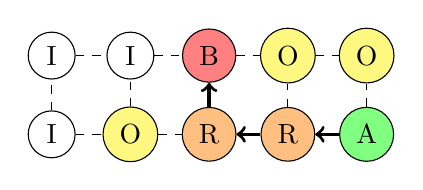
\begin{tikzpicture}
  \tikzstyle{router}=[circle, draw, fill=orange!50,text=black]
  \tikzstyle{child}=[circle, draw, fill=yellow!50,text=black]
  \tikzstyle{root}=[circle, draw, fill=red!50,text=black]
  \tikzstyle{source}=[circle, draw, fill=green!50,text=black]
  \tikzstyle{idle}=[circle, draw, text=black]

  \node[idle] (00) at (0,0) {I};
  \node[child] (10) at (1,0) {O};
  \node[router] (20) at (2,0) {R};
  \node[router] (30) at (3,0) {R};
  \node[source] (40) at (4,0) {A};

  \node[idle] (01) at (0,1) {I};
  \node[idle] (11) at (1,1) {I};
  \node[root] (21) at (2,1) {B};
  \node[child] (31) at (3,1) {O};
  \node[child] (41) at (4,1) {O};

  \path
  % Radio link
  (00.east) edge[dashed] (10.west)
  (10.east) edge[dashed] (20.west)
  (20.east) edge[dashed] (30.west)
  (30.east) edge[dashed] (40.west)

  (01.east) edge[dashed] (11.west)
  (11.east) edge[dashed] (21.west)
  (21.east) edge[dashed] (31.west)
  (31.east) edge[dashed] (41.west)

  (00.north) edge[dashed] (01.south)
  (10.north) edge[dashed] (11.south)
  (20.north) edge[dashed] (21.south)
  (30.north) edge[dashed] (31.south)
  (40.north) edge[dashed] (41.south)

  % Route link
  (40.west) edge[->, very thick] (30.east)
  (30.west) edge[->, very thick] (20.east)
  (20.north) edge[->, very thick] (21.south)
  ;

  \end{tikzpicture}

  \caption{Nœuds impactés par l'acheminement de paquets depuis le nœud A vers le nœud B.}
  \label{supervision:fig:estimators_overview}
\end{figure}

La Figure~\ref{supervision:fig:estimators_overview} représente une transmission d'un paquet entre un point A et B dans un \ac{LLN} typique et permet d'illustrer les nœuds impliqués dans un réseau maillé pour le routage d'un paquet.
Les liens en pointillés représentent les liens radios entre les différents nœuds et les nœuds représentés par un R sont les routeurs intermédiaires pour acheminer les paquets.
Les nœuds représentés par un O peuvent être sujets à des phénomènes d'Overhearing tandis que les nœuds représentés par un I ne sont pas affectés par cette transmission.

Le routeur de bordure peut observer les entêtes des paquets réseau qu'il route et extraire les sources et destinations pour chacun de ces paquets.
Soit $\mathcal{S}_i$ les paquets ayant le nœud $i$ pour source et  $\mathcal{D}_i$ les paquets ayant pour destination le nœud $i$.
Le routeur de bordure a une vue sur $\mathcal{S}_i$ et $\mathcal{D}_i$ pour chaque nœud dans le \ac{LLN}.

En outre, pour chaque paquet, le routeur connaît également sa taille et peut donc en connaissant la couche physique utilisée connaître le temps passé par un paquet sur le médium.
De plus, une couche liaison peut disposer d'un mécanisme d'acquittement par l'intermédiaire d'un paquet \texttt{ACK} envoyé par le destinataire lorsqu'une transmission a fonctionné.
Soit $T_p$ le temps pris par un paquet pour être transmis et $T_{\texttt{ACK}}$ le temps nécessaire pour transmettre un \texttt{ACK} au niveau de la couche liaison.

\subsubsection{Mesure passive ``étoilée''}
\label{supervision:noinfo_estimator}

Le routeur de bordure n'a pas forcément accès à la topologie d'un \ac{LLN}, ce qui peut par exemple arriver quand \ac{RPL} est utilisé en ``storing-mode''.
Dans ce cas, le routeur de bordure ne peut voir que la source et la destination dans l'entête d'un paquet qu'il doit router et agit comme si la topologie du réseau était étoilée.
Dans le scénario présenté sur la figure.~\ref{supervision:fig:estimators_overview}, l'estimation ``étoilée'' ne déduit que les temps de radios utilisés par les nœuds $A$ et $B$ en ignorant les autres nœuds impliqués.

\begin{align}
  \textrm{Tx}_i &= \sum_{p \in \mathcal{S}_i}{T_p} + \sum_{p \in \mathcal{D}_i}{T_{\texttt{ACK}}}\\
  \textrm{Rx}_i &= \sum_{p \in \mathcal{D}_i}{T_p} + \sum_{p \in \mathcal{S}_i}{T_{\texttt{ACK}}}
\end{align}

Ce type de supervision peut être adapté pour des topologies étoilées comme celles vues dans la section~\ref{gw:long_range}.
Cependant, dans le cas des scénarios maillés, cette méthode de mesure sous-estimera l'impact du routage intermédiaire et doit être complétée avec une connaissance de la topologie.

\subsubsection{Mesure passive ``maillée''}
\label{supervision:route_estimator}

Un routeur de bordure peut avoir la connaissance des routes descendantes vers les nœuds, c'est par exemple le cas quand \ac{RPL} est utilisé en ``non-storing mode''.
Dans ce cas, les routes descendantes sont utilisées pour inférer l'impact d'un paquet sur le \ac{LLN} de manière plus fine.
De plus, dans le cas où un nœud est configuré pour n'utiliser qu'un seul parent à la fois, la topologie des routes montantes est équivalente à celle descendante.

Dans le reste de cette thèse, il sera supposé que chaque nœud utilise exclusivement son parent préféré pour les routes montantes.


Ainsi lorsque les informations sur le routage sont disponibles il est possible de compléter la supervision passive pour prendre en compte l'impact causé par le relayage des paquets.
Dans le scénario présenté sur la figure.~\ref{supervision:fig:estimators_overview}, l'estimation ``maillée'' comptabilise les temps de radios utilisés par les nœuds $A$ et $B$ mais aussi ceux des nœuds routeurs (R).

Soit $\mathcal{F}_i$ l'ensemble des paquets qui sont routés par le nœud $i$ alors qu'il n'est ni la source ni le destinataire du paquet.

\begin{align}
  \textrm{Tx}_i &= \sum_{p \in \mathcal{S}_i \cup \mathcal{F}_i}{T_p}
                      + \sum_{p \in \mathcal{D}_i}{T_{\texttt{ACK}}}\\
  \textrm{Rx}_i &= \sum_{p \in \mathcal{D}_i \cup \mathcal{F}_i}{T_p}
                      + \sum_{p \in \mathcal{S}_i(t)}{T_{\texttt{ACK}}}
\end{align}

\paragraph{Remarque sur l'``over-hearing''}

Les nœuds ne peuvent pas savoir si une trame leur est destinée avant de la recevoir ainsi ils peuvent dépenser de l'énergie pour décoder une trame sans qu'elle ne leur soit destinée (``over-hearing'' en anglais).
Donc, la connaissance des routes n'est pas encore suffisante pour prévoir intégralement l'impact du trafic sur un \ac{LLN}, la supervision passive idéale prendrait également en compte les phénomènes d'over-hearing.

Il est possible d'envoyer ces informations en utilisant des paquets déjà existants (routage ou applicatif) et ainsi d'avoir à la passerelle ces informations par un mécanisme de ``piggy-backing''.
Ou bien, d'utiliser la connaissance des voisins qui peut être donnée par un administrateur dans le cas où les emplacements sont connus.

Cependant, la qualité du lien radio peut changer au cours du temps et la passerelle ne peut pas l'inférer sans rien demander aux nœuds.
Ainsi ce phénomène ne sera pas pris en compte lors de l'estimation passive de l'usage de la radio des nœuds, car aucune hypothèse n'est faite sur les informations que les nœuds envoient.

\subsection{Modélisation de l'utilisation de la radio d'un nœud}
\label{supervision:models}

La passerelle du fait de sa connexion avec les nœuds connaît la technologie sans-fil qui va être utilisée pour communiquer et peut donc fournir une modélisation de son impact.

L'interface radio est la principale consommatrice d'énergie dans la plupart des \ac{LLN}~\cite{antolin2013analysis}.
En particulier, l'énergie consommée par la transmission et la réception sont du même ordre~\cite{duarte2002analysis}.
Une utilisation importante de la radio implique dans les deux cas une grande quantité d'énergie consommée par le nœud.

L'objectif est de calculer le temps passé par chaque nœud pour transmettre un paquet $p$ de taille $\mathcal{L}(p)$ octets envoyé en unicast et avec un acquittement de taille constante.
Les modélisations suivantes se concentrent sur la radio \ieee{}, de plus, afin d'économiser de l'énergie, il est également pris pour hypothèse que les nœuds utilisent un mécanisme de cycle de veille.
ContikiMAC~\cite{dunkels11contikimac} dispose d'un cycle d'endormissement très économe en énergie~\cite{michel2014analyse}.
Il sera modélisé et utilisé par les nœuds.

\subsubsection{Impact de \ieee{}}

\ieee{} peut être utilisé de plusieurs façons différentes (taille courte ou longue d'adresse, avec ou sans couche \ac{MAC}, etc.)~\cite{baronti2007wireless}.
Cette section prend pour hypothèse que \ieee{} fonctionne avec le protocole \ac{CSMA/CA} et que le temps utilisé par un paquet individuel $p$ sur la radio est donné de la manière suivante:

\DeclarePairedDelimiter{\ceil}{\lceil}{\rceil}

\[T_p = \frac{\mathcal{L}(f)}{R} \ceil[\Big]{\frac{\mathcal{L}(p)}{L}}\]

où $\mathcal{L}(f)$ est la taille d'une trame de donnée complète \ieee{} (127 octets), $R = 250$ kbits/s est le débit du \ieee{}, $L$ est la charge utile (payload) maximale d'une trame de donnée \ieee{} (environ 89 octets avec les options usuelles) et $\mathcal{L}(p)$ la taille du message que l'on veut transmettre sur ce médium.
Une trame de donnée complète prend environ 4 ms pour être transmise.

Une trame d'acquittement \texttt{ACK} en \ieee{} est de taille constante (11 octets) et occupe donc la radio pendant $T_\texttt{ACK}$ = 0.352 ms.

Quand une source émet une trame, tous les nœuds en écoute qui sont à portée radio vont tenter de décoder la trame et devront la saisir complètement avant de vérifier qu'elle est correcte par sa somme de contrôle et qu'elle leur est destinée.
Il est possible qu'un voisin éteigne sa radio lorsqu'il détecte qu'il n'est pas concerné par cette transmission.
Néanmoins, chaque nœud réveillé dépense toujours une quantité minimale d'énergie, pour analyser une trame qui est émise par l'un de ses voisins.

Enfin, il est à noter que même quand aucun paquet n'est transmis, les nœuds utilisent leur radio afin de vérifier l'état du canal dans le but de recevoir un paquet.
Cependant, ce réveil ne peut être déduit implicitement de la part de la passerelle et rentre donc dans les phénomènes non couverts par la mesure passive.

\subsubsection{Impact de ContikiMAC}
\label{supervision:contikimac}

Afin de communiquer, deux nœuds ont besoin d'être actifs en même temps.
Cependant, mettre les nœuds en réception permanente est très coûteux car une radio en écoute du canal (``channel listening'') consomme une énergie non négligeable~\cite{park2005throughput}.
Ainsi afin d'économiser les réserves d'énergie des nœuds, les nœuds s'endorment régulièrement en utilisant des mécanismes de cycle de veille qui alternent phase de sommeil et phase d'activité.

L’objectif de  ContikiMAC~\cite{dunkels11contikimac} consiste à endormir les nœuds pendant une partie du temps afin d’économiser leur batterie et d’éviter les collisions dans les zones denses où plusieurs nœuds veulent transmettre simultanément.
Ce mécanisme de cycle de veille est notamment utilisé par Contiki~\cite{dunkels2004contiki} en raison de son efficacité à économiser de l'énergie et sa faible empreinte mémoire~\cite{michel2014analyse}.
Ainsi il sera utilisé comme référence de cycle de veille dans ce chapitre.

\begin{figure}[ht]
  \centering
  \includegraphics[width=.5\textwidth]{img/contikimac.png}
  \caption{Fonctionnement des réceptions avec ContikiMAC}
  \label{supervision:fig:contikimac}
\end{figure}

La Figure~\ref{supervision:fig:contikimac} illustre le fonctionnement de ContikiMAC.
Pour transmettre une trame de donnée (D), un émetteur l'envoie de manière répétée (``packet strobing'' en anglais) tant qu'une trame d'acquittement (A) n'est pas reçue de la part du récepteur.
Un récepteur va se réveiller périodiquement et faire une écoute du canal pour détecter la présence d'une trame (l'écoute du canal est représentée en bleu sur la figure).
Si aucune émission n'est détectée, le récepteur se rendort.
Quand une émission est détectée, le récepteur passe en réception pour recevoir la trame de donnée dans son intégralité puis, quand la trame de donnée est reçue, une trame d'acquittement est envoyée du récepteur vers l'expéditeur.

Dans le cas d'une trame destinée à tous les voisins (broadcast), elle est répétée sur toute la phase d'activité afin de s’assurer que tous les voisins l’ont reçue au moins une fois.
D'autre part, les voisins n'envoient pas un acquittement à la réception d'une trame envoyée en broadcast.

Si une trame est transmise sur le canal pendant la phase de réveil, le récepteur reste réveillé pour la recevoir sinon il se remet à l’état sommeil.
Lorsqu'un nœud reçoit une trame et qu'elle lui est effectivement destinée, il envoie un acquittement.

Pour optimiser sa transmission, le protocole ContikiMAC utilise une technique de verrouillage de phase.
Elle consiste à estimer la date de réveil du prochain saut pour une destination donnée à partir de la date de réception d’acquittement et de retarder le moment d’émission de paquets jusqu’à l’approche de cette date de réveil.
Cette technique peut économiser de l'énergie en réduisant la quantité de strobing nécessaire à l'envoi d'un paquet en ``synchronisant'' envois et phases de réveil.
Cependant, cette technique n'est pas parfaite, car les horloges internes des différents nœuds ne sont pas synchronisées et des décalages peuvent tout de même se produire~\cite{gonizzi2014rawmac}.

Toujours dans l’objectif d’augmenter la durée de la période de sommeil, le protocole ContikiMAC dispose d'un mécanisme de mise en sommeil rapide pouvant distinguer une transmission de paquet du bruit en comparant la période de l’activité à des longueurs types: (supérieure à la longueur maximale d’un paquet, etc.).
Si la période d'activité n'est pas due à une transmission, le nœud se rendort immédiatement.

Ainsi ContikiMAC permet d'économiser de l'énergie par de multiples techniques, mais cette économie se paye par l'envoi répété d'une trame.
Donc, il est nécessaire de comptabiliser ces retransmissions afin d'avoir une mesure implicite pertinente.

Soit $N_{\textrm{sender}}$ (respectivement $N_{\textrm{receiver}}$) le nombre de fois qu'une source (respectivement une destination) va transmettre (respectivement recevoir) un paquet avec ContikiMAC.

Puisque le destinataire se réveille en moyenne au milieu d'une transmission et attend le prochain essai d'envoi pour recevoir la trame complètement et envoyer son acquittement, le nombre de trames reçues par le destinataire peut être estimé à $N_{\textrm{receiver}} = 1.5$.

Estimer $N_{\textrm{sender}}$ est plus difficile, car cette grandeur dépend des conditions réseau (topologie, qualité du lien) et de la taille des trames.
Ainsi il est nécessaire d'avoir une estimation de ce paramètre afin de procéder à une estimation réaliste de l'utilisation de la radio.

L'expérience suivante est réalisée afin d'estimer le nombre moyen d'essais d'envoi d'une trame de donnée qu'un expéditeur va faire avant de recevoir une trame de confirmation.
Deux nœuds utilisant ContikiMAC sont mis à portée de transmission dans un environnement non bruité.
La source envoie en boucle un paquet de taille fixe qui induit de multiples retransmissions, puis elle attend l'acquittement du paquet et comptabilise le nombre d'essais réalisés avant de recevoir un acquittement et cela pour différentes tailles de paquets.
\ieee{} est utilisé comme simple couche liaison avec un entête pour les trames de données aussi réduit que possible (6 octets) les différentes tailles de trames sont obtenues en faisant varier la taille du message applicatif.
Une simulation simule le comportement de ce système pendant 10000 secondes et pour chaque taille de paquet, l'expérience est exécutée 10 fois avec une graine de générateur de nombre aléatoire différente à chaque fois.

\begin{figure}[h]
  \centering
  \includegraphics[width=.5\textwidth]{img/average_strobbing-crop.pdf}
  \caption{Nombre moyen de tentatives d'envois en fonction de la taille de la trame avec ContikiMAC.}
  \label{supervision:fig:average_strobing}
\end{figure}

La Figure~\ref{supervision:fig:average_strobing} représente la moyenne du nombre de transmissions $N_{\textrm{sender}}(f)$ nécessaires à l'envoi d'une trame $f$ ayant une taille de $\mathcal{L}(f)$ octets entre deux nœuds fonctionnant avec ContikiMAC.
Le nombre d'envois moyens nécessaires pour envoyer un long paquet est plus faible que pour en envoyer un court, car les trames longues mettent plus de temps pour être transmises et ont donc plus de chance d'être écoutées pendant un réveil du destinataire.
% En outre, comme les paquets \ac{ACK} ont une taille constante, le coût de réception pour la source est constant.
% Cette valeur est inférieure à celle de $N_{\textrm{receiver}}$ ainsi c'est donc l'expéditeur qui va dépenser le plus d'énergie quand ContikiMAC est employé.

On peut remarquer que la variance est également faible pour des trames de grande taille ce qui est également cohérent, car le nombre d'envois qu'il est possible de faire pour une trame de cette taille au cours d'un cycle complet est limité ainsi la variance est réduite. 

\section{Validation expérimentale}
\label{supervision:validation}

\subsection{Supervision passive}
\label{supervision:chain_results}

\begin{figure}[ht]
  \centering
  \begin{tikzpicture}

  % définition des styles
  \tikzstyle{child}=[circle, draw, fill=yellow!50,text=black]
  \tikzstyle{router}=[circle, draw, fill=orange!50,text=black]
  \tikzstyle{root}=[circle, draw, fill=red!50,text=black]

  % Réseau contraint
  \node[root] (root) {G};
  \node[router, left=of root] (1) {1};
  \node[router, left=of 1] (2) {2};
  \node[router, left=of 2] (3)  {3};
  \node[router, left=of 3] (4) {4};
  \node[router, left=of 4] (5) {5};
  \node[child, left=of 5] (6) {6};

\path

  (6.east) edge[->, thin] (5.west)
  (5.east) edge[->, thin] (4.west)
  (4.east) edge[->, semithick] (3.west)
  (3.east) edge[->, thick] (2.west)
  (2.east) edge[->, very thick] (1.west)
  (1.east) edge[->, ultra thick] (root.west)
  ;

  \end{tikzpicture}

  \caption{Topologie réseau utilisée pour mesurer la précision de la mesure implicite et passive}

  \label{supervision:fig:topology_chain}
\end{figure}

Une topologie chaînée à 7 nœuds comme représentée sur la Figure~\ref{supervision:fig:topology_chain} est utilisée pour tester le mécanisme décrit ci-dessus.
Dans cette configuration, les nœuds ne peuvent envoyer et recevoir de  paquets que de la part de leurs voisins adjacents.
Tous les paquets remontent vers la passerelle représentée par un G sur la figure.

Les nœuds utilisent le système Contiki~\cite{dunkels2004contiki}, \ieee{} pour communiquer et ContikiMAC comme mécanisme de cycle de veille.
\ac{RPL}~\cite{rfc6550} est le protocole de routage utilisé et il est configuré en non-storing mode, c'est-à-dire qu'il a accès à toute la topologie réseau et en particulier aux routes descendantes.

Durant 200 secondes, chaque nœud envoie au \ac{LBR} un paquet \ac{UDP} à chaque seconde avec une charge utile de 10 octets ce qui induit une trame de 69 octets chaque seconde.
Le trafic applicatif d'un nœud démarre lorsqu'il joint la topologie réseau, il a alors un parent qui est son voisin adjacent.

D'après les résultats expérimentaux (Figure. \ref{supervision:fig:average_strobing}), l'utilisation de ContikiMAC induit qu'une trame de 69 octets est émise en moyenne 3,76 fois avant d'être reçue.
Le mécanisme de mesure implicite tient compte de ce phénomène et l'applique à chaque routeur intermédiaire afin que l'utilisation de la radio soit en accord avec ce résultat.

Les temps de transmission et de réception des nœuds sont obtenus par l'utilisation du simulateur et de Powertracker~\cite{dunkels2011powertrace} qui permet d'obtenir le temps passé dans chaque état de transmission radio pour chaque nœud avec une résolution de $1 \mu s$.
Puisque la passerelle est toujours éveillée, elle reçoit donc du premier coup toutes les trames: $N_{\textrm{receiver}} = 1$.

\subsubsection{Analyse de l'impact de la profondeur}
\label{supervision:depth_analysis}

\begin{figure}[ht]
  \begin{subfigure}{0.5\textwidth}
    \includegraphics[width=\textwidth]{img/pdr_depth.pdf}
    \caption{Packet Delivery Ratio (PDR).}
    \label{supervision:fig:pdr_depth}
  \end{subfigure}
  \begin{subfigure}{0.5\textwidth}
    \includegraphics[width=\textwidth]{img/strobes_depth.pdf}
    \caption{Tentatives d'envois de paquets par profondeur.}
    \label{supervision:fig:strobes_depth}
  \end{subfigure}
  \caption{Impact de la profondeur}
\end{figure}

\paragraph{\ac{PDR}}

La figure Fig.~\ref{supervision:fig:pdr_depth} représente le ratio de succès de transmission de paquets applicatifs pour chaque nœud en fonction de la distance à la racine en nombre de sauts.
Cette figure montre la proportion du trafic applicatif que la passerelle peut effectivement voir.
Le ratio de paquets acheminés n'est pas uniforme sur tout le \ac{LLN} et les nœuds qui ne sont pas connectés directement à une racine souffrent de pertes de paquets non négligeables malgré un trafic faible en raison d'un grand nombre de retransmissions de paquets.

Le routeur de bordure n'utilise pas ContikiMAC car dans les hypothèses de l'expérience, il n'est pas contraint en énergie et peut donc rester éveillé en permanence.
Ainsi, tous les paquets issus du nœud 1 sont reçus prouvant que ContikiMAC induit des pertes et nuit à la fiabilité des transmissions pour les nœuds plus éloignés.

Puisqu'un paquet peut être perdu à chaque fois qu'il traverse un routeur fonctionnant avec ContikiMAC, traverser de nombreux routeurs augmente la probabilité que les paquets soient perdus, car \ac{UDP} ne fournit aucun mécanisme de fiabilité.
Ce phénomène est confirmé par la Figure~\ref{supervision:fig:pdr_depth} où la quantité de paquets arrivant à la racine semble décroître globalement à mesure qu'on s'en éloigne.

\paragraph{Retransmissions de paquets (``Packet strobing'')}

La Figure~\ref{supervision:fig:strobes_depth} représente le nombre moyen d'envois de paquets i.e. le nombre de tentatives que va faire chaque nœud pour envoyer une trame à son parent.

Les valeurs obtenues précédemment restent expérimentalement proches de la valeur de 3,76 obtenue expérimentalement (Figure \ref{supervision:fig:average_strobing}).
Cependant, la variance est forte et le nombre de tentatives tend à augmenter à mesure que l'on s'éloigne de la racine.
Cette variance peut être expliquée par la variance obtenue pour des trames de 69 octets sur l'expérience de calcul des $N_{sender}$.

La convergence vers la valeur normale de 3,76 pour les nœuds proches de la racine s'explique par l'augmentation du trafic réseau sur ces nœuds: ils doivent relayer les paquets provenant de tous les autres nœuds.
Ainsi, leur rythme d'envoi se rapproche de celui de l'expérience de strobing où la source envoyait autant de paquets que possible vers un destinataire en s'assurant de son acquittement.
Pour un nœud situé en bout de chaîne et n'ayant donc aucune charge de routage, un plus grand décalage entre les cycles d'éveils est présent et explique ainsi les retransmissions supplémentaires.

Enfin, au sujet du nœud qui est connecté à la passerelle directement, la quantité moyenne d'envois est très proche de 1 avec une variance faible, ce qui est logique puisque par hypothèse la racine est toujours éveillée et peut donc recevoir immédiatement les transmissions qui en viennent.
Cependant, ce n'est pas le cas des nœuds se situant juste avant le nœud 1, qui reçoivent une quantité importante de trafic, mais qui ne peuvent pas la router avec la même efficacité (temporisation, ``buffering'', etc.).

\subsubsection{Analyse de l'impact des protocoles}
\label{supervision:protocols_analysis}

Connaître la répartition des protocoles au cours du temps permet de savoir la proportion de ressources investies dans le maintien du réseau et celle investie dans un but applicatif à valeur ajoutée.

\begin{figure}[ht]
  \begin{subfigure}{0.5\textwidth}
    \includegraphics[width=\textwidth]{img/protocol_repartition_depth.pdf}
    \caption{Répartition des protocoles par profondeur.}
    \label{supervision:fig:protocol_repartition}
  \end{subfigure}
  \begin{subfigure}{0.5\textwidth}
    \centering
    \includegraphics[width=\textwidth]{img/repartition_protocol.pdf}
    \caption{Évolution de la répartition des protocoles (statistiques par fenêtres de 25 secondes.}
    \label{supervision:fig:protocol_repartition_time}
  \end{subfigure}%
  \caption{Impact des protocoles}
\end{figure}

\paragraph{Répartition des protocoles}

La Figure~\ref{supervision:fig:protocol_repartition} met en évidence que la quantité de trafic lié au protocole de routage est relativement homogène pour tous les nœuds.
Ce phénomène est lié à la topologie et au fonctionnement de \ac{RPL}: les nœuds n'envoient de paquets de routage qu'à un seul parent à la fois ainsi le trafic de routage est le même pour tous les nœuds du réseau.

\paragraph{Évolution au cours du temps}

La Figure~\ref{supervision:fig:protocol_repartition_time} met en évidence l'évolution typique de la répartition des protocoles au cours du temps.
La charge liée au protocole de routage est très importante lors du démarrage du réseau, car aucune route n'est alors disponible.
Ainsi l'essentiel du trafic observé correspond à des paquets \ac{RPL} qui sont utilisés pour mettre à jour les routes sur chaque nœud.

\ac{RPL} étant proactif, les routes sont construites et entretenues en permanence, ainsi même après la construction de la topologie, du trafic \ac{RPL} est toujours émis.
Cependant, le mécanisme de ``Trickle'' réduit la quantité de paquets émis pour maintenir la topologie qui est observée.

Cette évolution du trafic permet de déduire qu'un mécanisme n'ayant pas la connaissance des routes manquerait non seulement l'impact du relayage sur les routeurs dans la topologie, mais aussi la charge impliquée par la construction des routes qui est non négligeable même dans le cas d'une topologie simple comme celle d'une chaîne.

Cependant, le trafic applicatif est majoritaire lorsque le réseau est stable, ainsi l'approche par supervision passive peut être explorée, car l'essentiel du trafic a vocation à passer par le routeur de bordure.

\subsection{Précision de la mesure passive de l'utilisation de la radio}

Le mécanisme d'estimation se déclenche quand toutes les routes sont établies et qu'un trafic réseau est observé à la passerelle.
L'estimation du temps radio va alors fournir une estimation pour le temps passé en transmission et en réception pour chaque nœud.

On appelle \emph{précision} $\delta = \frac{\widehat{X}}{X}$ le rapport entre l'estimation d'une grandeur $\widehat{X}$ et sa valeur réelle $X$ qui est mesurée dans le simulateur.
Cette métrique permet d'interpréter facilement les grandeurs trouvées: $\delta \leq 1$ (respectivement $\delta \geq 1$) signifie que l'estimation sous-estime (respectivement surestime) la grandeur.
Cette section mesure la précision des estimations passives pour les cas d'estimation ``étoilée'' (où la topologie de routage est inconnue) et ``maillée'' (où la topologie de routage est connue).

\subsubsection{Précision en fonction de la topologie}

\begin{figure}[ht]
  \begin{subfigure}{0.5\textwidth}
    \centering
    \includegraphics[width=\textwidth]{img/global_noinfo.pdf}
    \caption{$\delta$ total global pour l'estimation ``étoilée''}
    \label{supervision:fig:global_noinfo}
  \end{subfigure}
  \begin{subfigure}{0.5\textwidth}
    \centering
    \includegraphics[width=\textwidth]{img/global_route.pdf}
    \caption{$\delta$ total global pour l'estimation ``maillée''}
    \label{supervision:fig:global_route}
  \end{subfigure}
  \caption{$\delta$ total et global par profondeur}
  \label{supervision:fig:global}
\end{figure}

La Figure~\ref{supervision:fig:global} montre que la précision obtenue à la fin de la simulation pour chaque nœud est sous-estimée.
Ce phénomène est attendu, car la mesure implicite ne peut inférer tous les phénomènes, de plus l'approche proposée n'introduit pas de mécanismes ad hoc pour augmenter les estimations.

Dans le cas de l'estimation ``étoilée'', $\delta$ est homogène pour l'ensemble des nœuds qui ont pour charge de router des paquets qui ne leur sont pas destinés comme le montre la Figure~\ref{supervision:fig:global_noinfo}.
C'est cohérent avec la nature de l'estimation ``étoilée'' qui ne prend pas en compte toute la charge liée au routage.
De plus, la réception est plus sous-évaluée que la transmission, car elle ne prend en compte que la réception des trames d'acquittement qui représentent un volume très restreint sauf pour le nœud 6 qui n'a pas d'autre charge de réception.

Dans le cas de l'estimation ``maillée'', $\delta$ est plus élevé, car l'utilisation de la radio liée aux retransmissions est prise en charge ainsi une plus grande part du trafic est déduite des observations passives.
On remarque un net progrès pour la réception qui d'une part est régulière à prévoir avec ContikiMAC ($N_{receiver} = 1.5$) et d'autre part parce que le volume de routage est plus important.

Les erreurs d'estimations restent cependant importantes, car dans les deux cas, une part importante du trafic n'est pas inféré (pertes de paquets, variance du strobbing, trafic de routage local non transmis à la passerelle, etc.).

En outre, la mesure implicite ``étoilée'' ou ``maillée'' est identique pour le nœud feuille par construction, car aucune charge de routage ne lui est appliqué dans les deux cas.

\subsubsection{Évolution de $\delta$ au cours du temps}

Cette section étudie l'évolution de $\delta$ au cours du temps afin d'affiner la compréhension des facteurs pouvant expliquer la sous-estimation obtenue dans la section précédente.
Les résultats suivants sont obtenus en découpant l'expérience sur des intervalles de 20 secondes.
$\delta$ est alors le temps de radio estimé sur le temps réel dans cet intervalle uniquement.

\paragraph{Estimation ``étoilée''}

\begin{figure}[h]
  \centering
  \begin{subfigure}{0.3\textwidth}
    \includegraphics[width=\textwidth]{img/evolution_noinfo_1.pdf}
    \caption{Profondeur: 1}
    \label{supervision:fig:noinfo_1}
  \end{subfigure}
  \begin{subfigure}{0.3\textwidth}
    \includegraphics[width=\textwidth]{img/evolution_noinfo_2.pdf}
    \caption{Profondeur: 2}
    \label{supervision:fig:noinfo_2}
  \end{subfigure}
  \begin{subfigure}{0.3\textwidth}
    \includegraphics[width=\textwidth]{img/evolution_noinfo_3.pdf}
    \caption{Profondeur: 3}
    \label{supervision:fig:noinfo_3}
  \end{subfigure}

  \begin{subfigure}{0.3\textwidth}
    \includegraphics[width=\textwidth]{img/evolution_noinfo_4.pdf}
    \caption{Profondeur: 4}
    \label{supervision:fig:noinfo_4}
  \end{subfigure}
  \begin{subfigure}{0.3\textwidth}
    \includegraphics[width=\textwidth]{img/evolution_noinfo_5.pdf}
    \caption{Profondeur: 5}
    \label{supervision:fig:noinfo_5}
  \end{subfigure}
  \begin{subfigure}{0.3\textwidth}
    \includegraphics[width=\textwidth]{img/evolution_noinfo_6.pdf}
    \caption{Profondeur: 6}
    \label{supervision:fig:noinfo_6}
  \end{subfigure}
  \caption{Évolution de $\delta$ pour une estimation ``étoilée''}
  \label{supervision:fig:noinfo}
\end{figure}

La Figure~\ref{supervision:fig:noinfo} détaille pour chaque nœud l'évolution de $\delta$ pour une estimation ``étoilée''.
La sous-estimation continue, car les processus non visible depuis la passerelle (routage des paquets, pertes de paquets, etc.) continuent au cours de l'expérience.

Les nœuds situés à une plus grande profondeur relaient moins de paquets ainsi leur $\delta$ augmente, car une plus grande proportion de leur trafic applicatif est connue par le routeur de bordure au fur et à mesure de l'expérience.
D'autre part, $\delta$ augmente au cours du temps, car le trafic applicatif qui est celui inféré par la mesure passive prend une part plus importante au cours du temps (\ref{supervision:fig:protocol_repartition_time}).

\paragraph{Estimation ``maillée''}

\begin{figure}[h]
  \centering
  \begin{subfigure}{0.3\textwidth}
    \includegraphics[width=\textwidth]{img/evolution_route_1.pdf}
    \caption{Profondeur: 1}
    \label{supervision:fig:route_1}
  \end{subfigure}
  \begin{subfigure}{0.3\textwidth}
    \includegraphics[width=\textwidth]{img/evolution_route_2.pdf}
    \caption{Profondeur: 2}
    \label{supervision:fig:route_2}
  \end{subfigure}
  \begin{subfigure}{0.3\textwidth}
    \includegraphics[width=\textwidth]{img/evolution_route_3.pdf}
    \caption{Profondeur: 3}
    \label{supervision:fig:route_3}
  \end{subfigure}

  \begin{subfigure}{0.3\textwidth}
    \includegraphics[width=\textwidth]{img/evolution_route_4.pdf}
    \caption{Profondeur: 4}
    \label{supervision:fig:route_4}
  \end{subfigure}
  \begin{subfigure}{0.3\textwidth}
    \includegraphics[width=\textwidth]{img/evolution_route_5.pdf}
    \caption{Profondeur: 5}
    \label{supervision:fig:route_5}
  \end{subfigure}
  \begin{subfigure}{0.3\textwidth}
    \includegraphics[width=\textwidth]{img/evolution_route_6.pdf}
    \caption{Profondeur: 6}
    \label{supervision:fig:route_6}
  \end{subfigure}
  \caption{Évolution de l'$\delta$ pour une estimation ``maillée''}
  \label{supervision:fig:route}
\end{figure}

L'estimation maillée est meilleure sur tous les intervalles de temps, ce qui est attendu, car elle comptabilise la charge de routage sur chacun de ces intervalles en plus de l'estimation étoilée.

D'autre part, l'estimation s'améliore au cours du temps, car non seulement le trafic applicatif devient majoritaire au cours du temps comme montré sur la Figure~\ref{supervision:fig:protocol_repartition_time} mais en plus la charge de routage intermédiaire qu'il induit est également comptabilisée.

% Discussion

Cependant, l'erreur d'estimation est encore forte en raison des pertes de paquets et des variations de la quantité de ``strobbing'' nécessaire pour transmettre un paquet à chaque saut.
Ainsi si la quantité de strobbing est sous-estimée, sur chaque saut l'impact de chaque paquet sur l'estimation de la radio est grandement perturbé.

Afin de limiter le strobbing, une solution serait d'avoir des trames aussi remplies que possible (par exemple avec des informations au sujet des nœuds.).
Ainsi, la quantité de strobbing nécessaire serait beaucoup plus faible, car les trames seraient détectées au bout d'un faible nombre de tentatives.

Une autre solution possible consiste à envoyer à intervalles réguliers des informations de ``recalibrations'' afin de recaler les estimations pour fournir des valeurs correctes.

\section{Mesures explicites}
\label{supervision:explicite}

La passerelle peut effectuer une mesure passive du temps passé par les nœuds du \ac{LLN} en transmission et en réception.
Cependant, les paquets perdus, retransmis ou non routés vers la passerelle ne sont pas comptabilisés avec cette méthode qui induit donc un biais.

Ainsi des mécanismes de mesure active semblent inévitables pour obtenir une information fiable.
Ces messages peuvent être envoyés à la passerelle par ``piggybacking'' ou être mis dans les paquets du protocole de routage utilisé.

Cependant, le rythme de ces mesures doit être modéré afin de limiter la consommation de ressources qu'il induit.
Ainsi si les temps entre deux envois de mesures explicites sont longs, la mesure implicite de la radio précédemment introduite peut fournir une approximation entre ces deux envois.

Quand la passerelle reçoit une mesure explicite au temps $t$ elle recalcule son estimation pour la grandeur $\widehat{X}$ de la manière suivante:

\begin{align}
  \widehat{X}(t) &= X(t_r) + \epsilon(t_r)\frac{t - t_r}{T}\\
  \epsilon(t_r) &= \alpha (X(t_r) - \widehat{X}(t_r)) + (1 - \alpha)\epsilon(t_{r-1})
  \label{supervision:eqn:bias}
\end{align}

où $t_r$ et $t_{r-1}$ sont les deux dernières dates de réception de mesure active.
$T$ désigne le temps entre chaque mesure explicite reçue.
$X(t_r)$ désigne la valeur obtenue par mesure explicite à l'instant $t_r$.
$\epsilon(t_r)$ est l’estimation de l'erreur apprise des précédents messages de mesure active~\footnote{Par convention: $\epsilon(0) = 0$}.
Cette erreur est calculée par une \ac{EWMA} de paramètre $\alpha$~\cite{mckinney2012python}.
Le coefficient $\alpha$ compris entre 0 et 1 représente le degré de décroissance des erreurs des valeurs passées.
Une valeur de $\alpha$ importante réduira plus rapidement l'importance des observations passées.
A un instant $t$, l'erreur est prise proportionnellement au temps depuis la dernière mesure explicite reçue.


% $\frac{X(t_r) - X(t_{r-1})}{t_r - t_{r-1}}$ représente la tendance de la grandeur $X$. 
% Le paramètre $\alpha$ désigne la proportion de l'estimation 

\subsection{Validation expérimentale}

\begin{figure}[ht]
  \centering
  \includegraphics[width=0.5\textwidth]{img/topology_tree.png}
  \caption{Topologie réseau et radio.}
  \label{supervision:fig:topology_tree}
\end{figure}

Cette méthode de recalibration des mesures passives est évaluée en utilisant une topologie représentée sur la Figure~\ref{supervision:fig:topology_tree} composée de 21 nœuds envoyant des paquets applicatifs à la racine chaque seconde pendant 200 secondes.
Les messages contenant des mesures exactes des temps mesurés par le nœud passé dans chaque état de transmission sont envoyés par les nœuds par un mécanisme de publish-subscribe pour économiser le coût d'une requête.
La fréquence de ces envois de recalibrations est réglée par l'administrateur.

Comme vu dans les validations précédentes, le réseau est peu régulier et les phénomènes de strobing ont une grande variance.
Ainsi, afin de ne pas réagir trop brutalement aux changements d'une mesure et de privilégier les tendances de fond, le paramètre de décroissance de l'\ac{EWMA} est mis à $\alpha = 0.25$.

\paragraph{Erreur relative globale}

\begin{figure}[ht]
  \centering
  \includegraphics{img/ratio_recalibration_global-crop.pdf}
  \caption{Erreur d'estimation globale pour une topologie en arbre avec et sans recalibration dynamique (toutes les 25 secondes).}
  \label{supervision:fig:tree_calibration}
\end{figure}

La Figure~\ref{supervision:fig:tree_calibration} montre le rapport entre la valeur estimée et la valeur réelle moyenne quand des messages de supervisions périodiques sont envoyés par les nœuds toutes les 25 secondes.
A chaque mesure explicite, l'estimateur intègre l'erreur moyenne des précédentes mesures et converge ainsi vers une estimation correcte.
On observe également que les pentes des estimations après chaque recalibrations sont moins grandes, car l'estimateur apprend son biais qui est supposé constant pendant l'expérience.
Ainsi on obtient une estimation qui a tout temps est capable de produire une estimation du temps passé en transmission et en réception.

\paragraph{Fréquence de recalibrage}

\begin{figure}[ht]
  \centering
  \includegraphics{img/ratio_recalibration-crop.pdf}
  \caption{Erreur relative pour différents intervalles de supervision active.}
  \label{supervision:fig:frequencies_error}
\end{figure}

La Figure~\ref{supervision:fig:frequencies_error} montre l'erreur moyenne globale obtenue par le mécanisme avec une estimation étoilée en fonction des périodes entre chaque message de supervision active.
Sur une expérience durant 200 secondes, n'avoir qu'une seule recalibration à mi-parcours (100 secondes) n'est pas suffisant pour avoir une bonne précision.
Ce phénomène est attendu, car même si la mesure active permet de connaître l'état exact d'un nœud, n'avoir cette information qu'une fois au cours de l'expérience n'est pas suffisant.
Lorsque les recalibrations sont plus fréquentes, la précision est meilleure, mais au prix d'un plus grand nombre de paquets émis.

\subsection{Travaux en cours}
\label{supervision:ingoing}

De nouveaux travaux~\footnote{Entrepris lors d'un séjour au \ac{SICS} entre août et septembre 2015 en collaboration avec Simon Duquennoy.} étendent les recherches de ce chapitre.
Leur objectif est de trouver des schémas de supervision explicites plus économes en énergie que les méthodes systématiques et cycliques présentes dans l'état de l'art.
Partant du constat que la supervision active est toujours nécessaire et ne peut pas être facilement substituée, l'objectif consiste à trouver une méthode optimale de supervision permettant de réduire son coût autant que possible.

\subsubsection{Mesure systématique}

Une supervision cyclique impose à chaque nœud d'envoyer des rapports sur son état à intervalles réguliers.
Le problème de cette approche est que son coût augmente linéairement avec le nombre de nœuds présents dans le \ac{LLN} et peut être coûteux en ressources si la fréquence d'envoi est trop importante.

Une première piste de recherche en cours d'investigation consiste à diminuer le nombre d'informations envoyées à mesure que le comportement d'un nœud est stable.
Cette méthode s'inspire de la méthode utilisée par Trickle~\cite{rfc6206} dans le protocole \ac{RPL} qui diminue le nombre de messages de routage à mesure que le routage devient stable.
L'évaluation de cette méthode notamment dans le cas de réseau instable et la comparaison avec des méthodes cycliques est l'un des premiers objectifs de ces nouveaux travaux.

\subsubsection{Mesure ciblée dynamique}

Une seconde approche consiste à choisir dynamiquement quel nœud interroger afin d'améliorer le modèle que la passerelle a d'un \ac{LLN}.
Cependant, la passerelle ne peut savoir si l'état d'un nœud diverge de son modèle avant de le lui demander.
Ainsi la passerelle a le choix entre conserver un modèle incertain et ne pas solliciter un nœud donné afin d'économiser des ressources ou bien payer le coût d'une mesure active quitte à ce qu'elle ne soit pas pertinente.
Cette problématique d'exploration contre exploitation~\cite{liu1112intrusion} est connue et explorée dans le domaine de l'apprentissage renforcé~\cite{posen2012chasing}.

Cette approche consiste à attribuer une valeur à l'information acquise quand la passerelle obtient une mesure venant d'un nœud et de mesurer ce gain au coût de son obtention.
L'objectif est alors de maximiser la valeur des informations obtenues tout en minimisant le coût nécessaire pour l'obtenir.

Cependant, cette approche est complexe, car un nœud qui est instable temporairement peut présenter temporairement un gros gain d'information si la passerelle le choisit.
Ainsi, il peut être tentant pour la passerelle de redemander plus régulièrement alors que le gain d'information était seulement temporaire.

Des approches venant du monde de la détection d'anomalies~\cite{liu1112intrusion} et utilisant des \ac{RMAB} sont une piste en cours d'exploration.

\subsubsection{Méthode d'évaluation}

Le protocole d'évaluation de ces techniques serait d'évaluer l'information obtenue avec plusieurs méthodes (aléatoire, cyclique, dynamique, etc.) avec une approche de type oracle qui trouverait toujours la meilleure information à demander pour mettre à jour un modèle donné.
Des évaluations sur des nœuds émulés et réels sont en cours de réalisation.

\section{Conclusion}
\label{supervision:conclusion}

% Résumé

La supervision d'un \ac{LLN} est importante pour garantir sa fiabilité et doit être réalisée en consommant aussi peu de ressources que possible.
Ce chapitre montre comment une estimation implicite de l'utilisation de la radio peut être réalisée en utilisant la topologie réseau et le trafic observé au niveau de la passerelle pour inférer les temps d'utilisation de la radio de chaque nœud sans les solliciter.

% Avantages

La supervision passive peut fournir de manière transparente une estimation de l'utilisation de la radio qui peut ensuite être utilisée pour détecter des problèmes (retransmissions trop importantes, routeurs intermédiaires surchargés).
Elle peut être utile dans le cas de nœuds contraints à l'extrême et qui ne peuvent pas fournir d'informations sur leur fonctionnement à une station de base ou bien pour implémenter des méthodes de supervision transparente pour les nœuds.
Sa précision augmente à mesure que le réseau devient stable et le trafic prévisible.
La connaissance de la topologie dans des scénarios maillés multi sauts est cruciale, car elle permet de prendre en considération les retransmissions effectuées par les nœuds routeurs.

% Limitations

Cependant, la supervision passive comporte plusieurs limitations, d'une part, les paquets émis localement ou perdus sont ignorés et induisent donc un biais qui tend à fournir des estimations sous-évaluées du temps d'utilisation de la radio.
D'autre part, l'utilisation de cycle de veille asynchrone est certes efficace pour économiser de l'énergie, mais se paye par une absence d'informations sur le nombre de retransmissions qu'un émetteur va faire pour transmettre une trame.
De plus, ce phénomène est amplifié dans des scénarios multi sauts où les erreurs d'estimations peuvent se faire sur chacun des sauts.
Ainsi si la précision n'est pas jugée suffisamment bonne pour être utilisée en pratique il faut payer le coût de mesures explicites.
Cependant, même dans ce cas, la supervision passive peut fournir des estimations de l'utilisation de la radio entre les mesures explicites.

% Amélioration

La supervision passive peut s'appliquer à des couches \ac{MAC} beaucoup plus régulières et fiables comme~\ac{TSCH} où les endormissements et les réveils sont déterministes (supprimant ainsi les phénomènes d'over-hearing, etc.).
Ces méthodes d'accès étant plus prévisibles, elles peuvent être inférées plus facilement.
Une ouverture possible de ces travaux serait de les adapter à ce type de couches \ac{MAC}.

Des améliorations sont également possibles au niveau de l'inférence de l'impact des protocoles de routage lorsque la construction des routes est fiable (acquittement au moment de la construction des routes descendantes).
Ainsi, une fois les routes établies, le routeur de bordure aurait la possibilité d'inférer le coût en transmission nécessaire pour l'établissement de cette topologie.

% Le mot de la fin

Aussi sophistiquée que soit l'inférence, la mesure active est indispensable pour un système ayant de fortes contraintes de fiabilité.
La mesure passive n'a pas vocation à remplacer cette approche et se pose comme une source de métrique pouvant être déployée dans n'importe quelle condition et de manière transparente pour le \ac{LLN} afin de fournir un service minimum de supervision.


\section*{Publications}

  Rémy Léone, Jérémie Leguay, Paolo Medagliani, Claude Chaudet.
    \newblock {Tee: Traffic-based energy estimators for duty-cycled Wireless Sensor Networks}.
    \newblock {\em {IEEE International Conference on Communication (ICC)}}, page~6749-6754, Londres, 2015.
%!TEX root = ../main.tex

\chapter{Cache} % (fold)
\label{cha:cache}

\minitoc

\lipsum

\section{Introduction} % (fold)
\label{sec:cache_introduction}

\lipsum

% section introduction (end)

\section{Cache Architecture} % (fold)
\label{sec:cache_architecture}

\lipsum

% section cache_architecture (end)

\section{Experiments} % (fold)
\label{sec:cache_experiments}

\lipsum

% section experiments (end)

\section{Performance Measurements} % (fold)
\label{sec:performance_measurements}

\subsection{Reactivity to network changes} % (fold)
\label{sub:reactivity_to_network_changes}

\begin{itemize}
	\item Combien de temps me faut il pour me rendre compte qu'un noeud est indisponible ?
	\item Combien de temps me faut il pour détecter une panne ?
	\item Comment les durée de cache s'adaptent a un changement de réseau ?
	\item Quel est le délai pour détecter un gros problème dans le réseau et adapter le niveau de requêtes histoire de calmer le jeu?
	\item Quel est le délai entre un changement dans le réseau significatif et un recalcul des temps de caches.
	\item Est ce que l'on peut avoir des phénomènes d'oscillation du système ? Typiquement des requêtes qui passent puis ne passent plus à la même fréquence. Comment lutter contre ce problème s'il existe?
	\item L'impact de la topologie se présente de manière évidente dans le calcul du temps de cache.

	\item est ce que ce système dans le cas ou il se plante bloque des utilisateurs comme 
	un ascenseur ou bien c'est plutôt un escalier de tel sorte qu'il ne bloque pas les utilisateurs d'en trouver un autre si il se plante.

	\item La fonction économique que l'on va utiliser peut être modifié selon différents critères. Par exemple on peut avoir une répartition des poids différentes selon qu'un noeud a plus ou moins de voisins. Une autre approche consiste a prendre en compte la répartition des popularités des requêtes envoyées.

	\item Est ce que ça fonctionne avec des topologies aléatoires ? Changeante (Ajout ou perte de noeuds)?

	\item Est ce que le modèle continue de fonctionner dans le cas ou on a plusieurs routeurs de bordure.	

\end{itemize}

% subsection reactivity_to_network_changes (end)

% section performance_measurements (end)

\section{Conclusion} % (fold)
\label{sec:cache_conclusion}

\lipsum

% section conclusion (end)

\section{Publications} % (fold)
\label{sec:cache_publications}

% section cache_publications (end)

% chapter cache (end)

%!TEX root = ../main.tex

\chapter{Automated and reproducible experiments} % (fold)
\label{cha:automated_and_reproducible_experiments}

\minitoc

\section{Motivation} % (fold)
\label{sec:automation_motivation}

\cite{leone2013makesense}
\lipsum

% section automation_motivation (end)

\section{Ecosystem} % (fold)
\label{sec:automation_ecosystem}

\lipsum

\subsection{Performance evaluation} % (fold)
\label{sub:performance_evaluation}

\begin{itemize}
	\item Comment mesurer la performance d'un mécanisme d'automatisation ?
	\item Est ce que des comparaisons sont mêmes possibles ?
\end{itemize}

% subsection performance_evaluation (end)

% section automation_ecosystem (end)

\section{Publications} % (fold)
\label{sec:automated_publications}

% section automated_publications (end)

% chapter automated_and_reproducible_experiments (end)

\chapter{Conclusion} % (fold)
\label{cha:conclusion}

\section{Collaborations \& Contributions} % (fold)
\label{sec:collaborations_&_contributions}

\begin{itemize}
	\item Ajouter la contribution de Fadwa
\end{itemize}

% section collaborations_&_contributions (end)

\section{Further works} % (fold)
\label{sec:further_works}

\lipsum

% section further_works (end)

% chapter conclusion (end)

\cleardoublepage % Empty page before the start of the next part

%----------------------------------------------------------------------------------------
%	THESIS CONTENT - APPENDICES
%----------------------------------------------------------------------------------------

\appendix

% \chapter{Extraits de code source utilisés par Makesense}
\label{code}

\section{Approvisionnement d'une expérience par l'utilisation de gabarit}
\label{code:templating}

Les gabarits sont des fichiers qui sont utilisés comme modèle pour produire d'autres fichiers.
L'objectif de l'utilisation de gabarit est de pouvoir générer de manière expressive des fichiers arbitrairement complexes et imbriqués qui vont être dynamiquement rendu.

Les fichiers sont produits en utilisant un moteur de rendu qui va fabriquer un nouveau fichier en injectant des variables données aux emplacements annoncées par des balises propres au langage de gabarit.
Un gabarit de fichier de configuration du simulateur COOJA utilisant le format du moteur de gabarit Jinja2 est ici présenté~:

\inputminted{django}{snippets/template.jinja2}

Ce gabarit permet d'utiliser par exemple les variables \texttt{title} ou bien \texttt{random\_seed} pour insérer du contenu.
Des mécanismes de boucles sont également disponibles afin de répéter un schéma de texte plusieurs fois.

L'utilisation d'un moteur de rendu se fait simplement en passant les variables par un simple appel de fonction (ici la méthode \texttt{render} de l'objet \texttt{main\_csc\_template}.
Ainsi générer un fichier de configuration peut être fait de manière expressive pour un grand nombre de nœuds.

\inputminted{python}{snippets/jinja2.py}

\section{Déploiement} % (fold)
\label{code:deploiement}

% \inputminted{python}{snippets/fabric.py}

% Fabric \cite{fabric} est une bibliothèque permettant de transmettre et d’exécuter des programmes sur des serveurs distants. 
% Depuis la ligne de commande, il va être possible de lancer différentes fonctions codées en Python. 

\section{Exécution}
\label{code:run}

\inputminted{python}{snippets/run.py}

Automatiser le lancement des processus nécessaire à l'exécution d'une expérience permet d'être sur de ne pas en oublier, de les lancer dans l'ordre et de les contrôler avec une grande flexibilité.
Dans la section de code présentée, chaque processus est lancé dans un ordre précis puis une fois que la simulation est terminée, les autres processus vont être terminés les uns après les autres.

\section{Mise en forme des résultats}
\label{code:parsing}

\inputminted{python}{snippets/parsing.py}

Au vu des volumétries mises en jeu lors de nos expériences nous avons préféré rester sur des solutions de traitements sur des fichiers \ac{CSV} pour leur facilité d'utilisation.

Afin d'avoir un traitement des données aisé, il est préférable de se ramener à des formats de fichiers textuels tel que le CSV. 
Ici, tshark est utilisé comme intermédiaire pour traduire un format binaire et extraire les informations les plus essentielles vers du texte.

Il est à noté que dès que cette transformation a été faite une fois, elle n'est jamais effectuée. 
En effet, le fait d'avoir sauvegardé les données dans un format intermédiaire permet de ne travailler qu'avec le CSV et de ne plus jamais avoir à faire une extraction d'information coûteuse et redondante. 

\section{Analyse} % (fold)
\label{code:analyse}

\inputminted{python}{snippets/pandas.py}

\subsection{Filtrage}

Nous obtenons ainsi en une ligne de code, un graphe représentant l'histogramme du nombre de paquets.

% Transformation triviales
Certaines transformations peuvent être triviales comme des conversions d'unités et des normalisations de valeurs. 
D'autres peuvent être la transformation des adresses \ac{MAC} vers des identifiants plus facilement compréhensibles, dépendant de l'expérience permettant de faire une cartographie géographique des événements dans le réseau.
Enfin, dans le cas de système très contraints où chaque octet de mémoire compte, des sorties textes compactes sont remplacées vers des noms plus détaillés ce qui facilite leur manipulation par un humain.
% Classification
Dans le cas d'un trafic réseau, il est nécessaire de pouvoir classifier chaque paquet transmis selon une série de critères qui vont permettre dans la prochaine phase d'analyse d'effectuer des traitements quantifiés.
Le fichier \ac{PCAP} obtenu précédemment contient toutes ces informations cependant ce format est binaire et n'est pas facilement exploitable sans des outils spécifiques.
Ainsi la phase de transformation d'un \ac{PCAP} consiste à le disséquer pour extraire les informations pertinentes de chaque paquet (source, destination, protocole,\ldots) puis d'envoyer ces informations sous la forme de données tabulées vers un fichier.
% Mise en forme
Une fois que toutes les transformations sont faites, des fichiers de données, dans un format standardisé comme \ac{CSV} sont disponibles pour être ensuite analysé en détail.

% section analyse (end)

\subsection{Fonctions agrégées}

Nous avons aussi géré l'analyse de données tabulaires telles que celles obtenues en analysant les paquets émis au cours de l'expérience.
Pour cela nous avons utilisé Pandas \cite{mckinney-proc-scipy-2010} qui est une bibliothèque Python permettant la manipulation et l'analyse des données tabulaires et de séries temporelles.
Cette bibliothèque permet la visualisation directe dans le notebook de grande quantité de données rangées en tableau et indexées.

En plus de la visualisation instantanée, Pandas permet aussi afin de raffiner encore plus une analyse en chaînant les traitements les uns derrière les autres.

\subsection{Traitements en masse}

L'analyse de résultat et la production de courbes peuvent être obtenus de manière ad-hoc en utilisant des outils de filtres (grep, awk, sed) sur les fichiers en entrées et des outils de graphes (gnuplot, tableur) pour produire les courbes.
Ces méthodes peuvent fonctionner dans des cas très simples, mais n'ont pas le même niveau de concision et d'expressivité dès qu'il s'agit de grouper ou d'effectuer des agrégations complexes sur plusieurs champs~\cite{racine2006gnuplot, williams2003gnuplot}.

\section{Présentation} % (fold)
\label{code:presentation}

\inputminted{python}{snippets/matplotlib.py}

L'intérêt d'utiliser ce genre de bibliothèque au lieu d'une solution ad-hoc telle que Gnuplot \cite{Gnuplot_4.4} vient du simple fait qu'elle peut être intégré directement à la suite des analyses et  traitements effectués sur les données de l'expérience. 
L'intégration est d'ores et déjà fournie à mesure que l'on travaille sur le notebook et les graphes peuvent être générés à la demande.

\section{Intégration continue (Travis-ci)} % (fold)
\label{code:ci}

\inputminted{yaml}{snippets/.travis.yml}

L'utilisation de Travis-ci peut être justifié par le fait qu'un tiers à priori non lié à une organisation ou un organisme de recherche peut être de bonne foi quant au caractère reproductible. 
L'intégration continue garantis que l'expérience pourra être reproduite.
Un point important de cette configuration est que les logiciels sont spécifiés avec une version (requierements.txt).
Ainsi, au cas où la bibliothèque viendrait à ne plus être maintenue ou comporterait des changements d'interfaces, il serait toujours possible de retrouver d'anciennes versions et reproduire l'expérience avant de la faire migrer vers de nouvelles versions.


Les fonctionnalités offertes par Travis-CI ont été réduites au cours de la rédaction de ce manuscrit invalidant une partie des décisions prises au départ pour les expériences nécessitant des interfaces virtuelles et l'injection de trafic venant de l'extérieur.

Ainsi nos expériences sont complètement documentée mais certaines parties ne peuvent plus être rejouées aujourd'hui dans des scénarios spécifiques.

Une migration vers des serveurs auto-hébergés~\cite{smart2011jenkins} permettant un contrôle total sur l'expérience sont une réponse aux limitations des solutions hébergées.

Nous avons utilisé Travis-ci~\cite{travis} comme serveur d'intégration continue en raison de la disponibilité de configurations pour l'environnement Contiki~\cite{contiki_travis} et de son intégration à Github qui héberge nos notebooks et propose un rendu direct en ligne.
Travis-ci étant une structure indépendante et ouverte, elle constitue un bon gage sur le fait que n'importe qui pourrait refaire l'expérience et s'assurer de nos résultats. 
Ainsi nous avons pu construire une démonstration présentant les différentes étapes présentées dans ce chapitre et les avons exécutées sur leurs serveurs. 

Ainsi, l'utilisation d'un testbed privé peut être une solution efficace pour effectuer régulièrement des tests d'intégration sur nœuds réels.
Une autre solution consiste à déployer des taches d'intégration dans des périodes creuses d'utilisation des testbed publics tels que la nuit ou les week-ends.

\chapter{Collaborations extérieures}
\label{collaborations}

\section{A scalable and self-configuring architecture for service discovery in the internet of things}

Les déploiements visés par l'\ac{IoT} mettent en jeu des milliards d'appareils, ainsi ces appareils rendent de nouvelles formes d’interactions entre les personnes et les objets possibles.

Afin de permettre des applications robustes et faciles d'utilisation sur ces objets, il est nécessaire de disposer de mécanismes qui minimisent (ou annule) le besoin d'intervention humaine extérieure pour leur configuration et leur maintenance.
Ces mécanismes doivent pouvoir gérer un grand nombre d'objets qui sera en forte croissance au cours des prochaines années.

Cette contribution propose un mécanisme d'auto-configuration basée sur une architecture pair-à-pair, visant de grands réseaux d'objets et permettant d'obtenir un service de découverte de ressource automatisée ne nécessitant aucune intervention humaine pour leur configuration.
En particulier, cette contribution se concentre sur les mécanismes de découverte de services locaux et globaux en montrant comment l'architecture proposée permet une interaction tout en préservant une indépendance opérationnelle.

L'efficacité de l'architecture proposée a été confirmée par des résultats expérimentaux obtenus sur déploiement réel.

\subsection*{Publication}

Simone Cirani, Luca Davoli, Gianluigi Ferrari, R{\'e}my L{\'e}one, Paolo
  Medagliani, Marco Picone, and Luca Veltri.
\newblock A scalable and self-configuring architecture for service discovery in
  the internet of things.
  \newblock 2014.

\section{Bounding Degrees on RPL}

\ac{RPL} est le protocole de routage standardisé par l'\ac{IETF} optimisé pour les \ac{LLN}s.

La stabilité de \ac{RPL} peut souffrir de pertes de paquets et causer une instabilité des routes.
La plupart des solutions dédiées à ce problème se concentrent sur l'amélioration des métriques utilisées pour construire les routes.
Ces métriques sont le plus souvent basées sur une évaluation de la qualité du lien radio.

BD-RPL (Bounded Degree RPL) adopte une nouvelle approche en ajoute une contrainte supplémentaire sur le nombre maximal d'enfants qu'un routeur \ac{RPL} peut accepter lors de la construction des routes.
Cette méthode utilise les paquets de signalisation utilisés par défaut par \ac{RPL} et ne nécessite pas une nouvelle signalisation.

BD-RPL est évalué sur simulateur et implémenté sur des nœuds réels qui ont montré une amélioration de la fiabilité des transmissions de 10\%, une réduction de la consommation énergétique de 50\% et une amélioration de 60\% du délai.

\subsection*{Publication}

Fadwa Boubekeur, L{\'e}lia Blin, Remy Leone, and Paolo Medagliani.
\newblock Bounding degrees on rpl.
\newblock In {\em Proceedings of the 11th ACM Symposium on QoS and Security for
  Wireless and Mobile Networks}, pages 123--130. ACM, 2015.

% \section{Tactique de supervision active économe en énergie} 

% Collaboration avec Simon en suède sur le bandit manchot

% Mettre quelques graphes.

% \part{Appendix} % New part of the thesis for the appendix

%----------------------------------------------------------------------------------------
%	POST-CONTENT THESIS PAGES
%----------------------------------------------------------------------------------------

\cleardoublepage\refstepcounter{dummy}
%\addcontentsline{toc}{chapter}{Acronyms} % Uncomment if you would like the acronyms to appear in the table of contents
\pdfbookmark[1]{Acronyms}{acronyms} % Bookmark name visible in a PDF viewer

%\markboth{\spacedlowsmallcaps{Acronyms}}{\spacedlowsmallcaps{Acronyms}}

\chapter*{Acronymes}

\begin{acronym}

\acro{$h$}{Cache Hit ratio}
\acro{$m$}{Cache Miss ratio}
\acro{6LBR}{6LoWPAN Border Router}
\acro{6LoWPAN}{IPv6 over Low power Wireless Personal Area Networks}
\acro{ACK}{Acknowledgement message}
\acro{AODV}{Ad-hoc On-demand Distance Vector}
\acro{API}{Application Programming Interface}
\acro{ARCEP}{Autorité de régulation des communications électroniques et des postes}
\acro{ARP}{Address Resolution Protocol}
\acro{BAN}{Body-Area Network}
\acro{BGP}{Border Gateway Protocol}
\acro{BLE}{Bluetooth Low-Energy}
\acro{BSS}{Basic Service Set}
\acro{CBOR}{Concise Binary Object Representation}
\acro{CCA}{Channel Check Assessment}
\acro{CCN}{Content Centric Network}
\acro{CoAP}{Constrained Application Protocol}
\acro{CON}{Confirmable message}
\acro{CoRE}{Constrained RESTful environment}
\acro{CPL}{Courant Porteur en Ligne}
\acro{CPU}{Central Processing Unit}
\acro{CSMA/CA}{Carrier Sense Multiple Access with Collision Avoidance}
\acro{CSV}{Comma Separated Values}
\acro{DAD}{Duplicate Address Detection}
\acro{DAG}{Directed Acyclic Graph}
\acro{DAO}{Destination Advertisement Object}
\acro{DHCP}{Dynamic Host Configuration Protocol}
\acro{DIO}{DODAG Information Object}
\acro{DIS}{DODAG Informational Solicitation}
\acro{DNS}{Domain Name System}
\acro{DODAG}{Destination-Oriented DAG}
\acro{DSL}{Domain Specific Language}
\acro{DTLS}{Datagram Transport Layer Security}
\acro{ETag}{Entity Tag}
\acro{ETX}{Expected Transmission Count}
\acro{EUI}{Extended Unique Identifier}
\acro{EWMA}{Exponentially Weighted Moving Average}
\acro{FFD}{Full Function Device}
\acro{HCP}{HTTP-CoAP proxy}
\acro{HTTP}{HyperText Transfer Protocol}
\acro{ICMPv6}{Internet Control Message Protocol v6}
\acro{ICN}{Information-Centric Networking}
\acro{IEEE}{Institute of Electrical and Electronics Engineers}
\acro{IETF}{Internet Engineering Task Force}
\acro{IGP}{Interior Gateway Protocol}
\acro{IHM}{Interaction Homme Machine}
\acro{IID}{Interface ID}
\acro{IoT}{Internet of Things}
\acro{IP}{Internet Protocol}
\acro{ISM}{Bande industrielle, scientifique et médicale}
\acro{JSON}{Javascript Serial Object Notation}
\acro{KP}{Knapsack Problem}
\acro{LAN}{Local Area Network}
\acro{LBR}{LoWPAN Border Router}
\acro{LLN}{Low-Power and Lossy Network}
\acro{LoWPAN}{Low-Power Wireless Personal Area Network}
\acro{LPWAN}{Low-Power Wide Area Network}
\acro{LRWPAN}{Low Rate Wireless Personal Area Network}
\acro{M2M}{Machine to Machine}
\acro{MAC}{Media Access Control}
\acro{MITM}{Man-in-the-middle}
\acro{MP2P}{Multi-point to point}
\acro{MQTT}{Message Queuing Telemetry Transport}
\acro{MTU}{Maximum transmission unit}
\acro{NAT}{Network Address Translation}
\acro{NDP}{Neighbor Discovery Protocol}
\acro{NFV}{Network Function Virtualization}
\acro{NON}{Non-confirmable message}
\acro{NSGA}{Non-dominated Sorting Genetic Algorithm}
\acro{NTP}{Network Time Protocol}
\acro{OEDL}{OMF Experiment Description Language}
\acro{OLSR}{Optimized Link State Routing protocol}
\acro{OMF}{Orbit Management Framework}
\acro{OSPF}{Open Shortest Path First}
\acro{OTA}{Over The Air}
\acro{P2MP}{Point to Multi-point}
\acro{P2P}{Point to Point}
\acro{PAN}{Personnal Area Network}
\acro{PCAP}{Packet CAPture}
\acro{PDF}{Portable Document Format}
\acro{PDR}{Packet Delivery Ratio}
\acro{PLSDU}{Physical Layer Service Data Unit}
\acro{PoE}{Power over Ethernet}
\acro{PSM}{Power Saving Mode}
\acro{QoS}{Quality of Service}
\acro{REST}{REpresentational State Transfer}
\acro{RFD}{Reduced Function Device}
\acro{RMAB}{Restless Multi-Armed Bandit}
\acro{ROLL}{Routing Over Low power and Lossy Networks}
\acro{RPCA}{Reverse Proxy Cache Adaptatif}
\acro{RPC}{Reverse Proxy Cache}
\acro{RPL}{Routing Protocol Layer}
\acro{RST}{Reset message}
\acro{SCADA}{Supervisory Control and Data Acquisition}
\acro{SICS}{Swedish Institute of Computer Science}
\acro{SOA}{Service Oriented Architecturei}
\acro{SQL}{Structured Query Language}
\acro{SSH}{Secure Shell}
\acro{TCP}{Transport Control Protocol}
\acro{TDD}{Test Driven Development}
\acro{TDMA}{Time Division Multiple Access}
\acro{Tee}{Traffic Energy Estimator}
\acro{TSCH}{Time-Slotted Channel Hopping}
\acro{TTL}{Time To Live}
\acro{UDP}{User Datagram Protocol}
\acro{URI}{Uniform Resource Identifier}
\acro{URL}{Uniform Resource Locator}
\acro{WSN}{Wireless Sensor Networks}
\acro{XML}{Extensible Markup Language}

% Traditional convention of sar

%\acro{rxpck/s}{Total number of packets received per second.}
%\acro{txpck/s}{Total number of packets transmitted per second.}
%\acro{rxkB/s}{Total number of kilobytes received per second.}
%\acro{txkB/s}{Total number of kilobytes transmitted per second.}
%\acro{txerr/s}{Total  number  of  errors  that happened per second while transmitting packets.}
%\acro{coll/s}{Number of  collisions  that  happened  per  second  while transmitting packets.}
%\acro{rxdrop/s}{Number  of received packets dropped per second because of a lack of space in linux buffers.}
%\acro{txdrop/s}{Number of transmitted packets dropped per second  because of a lack of space in linux buffers.}
%\acro{packet/s}{Number of network packets received per second.}
%\acro{udp/s}{Number of UDP packets received per second}
%\acro{tcp/s}{Number of TCP packets received per second.}
%\acro{hit/s}{Number of reply cache hits per second.}
%\acro{miss/s}{Number of reply cache misses per second.}

\end{acronym}  

\cleardoublepage% Bibliography

\label{app:bibliography} % Reference the bibliography elsewhere with \autoref{app:bibliography}

%\manualmark
%\markboth{\spacedlowsmallcaps{\bibname}}{\spacedlowsmallcaps{\bibname}} 
\refstepcounter{dummy}

%\addtocontents{toc}{\protect\vspace{\beforebibskip}} % Place the bibliography slightly below the rest of the document content in the table of contents
%\addcontentsline{toc}{chapter}{\tocEntry{\bibname}}

%\fancypagestyle{plain}{
%		\fancyhead{}
%        \fancyfoot[C]{\thepage}%
%		\renewcommand{\headrulewidth}{0pt}
%}%
\bibliographystyle{plain}%
\addcontentsline{toc}{chapter}{Bibliographie}%
%\bibliography{../../Bibliographie/biblio_votes/biblio_votes}
\bibliography{main}
 % Bibliography
% \cleardoublepage\input{tex/_specials/colophon} % Colophon
\cleardoublepage%\usepackage[left=1.3cm,top=0cm,right=1.3cm,bottom=1.2cm]{geometry}

% \usepackage{array}
% \usepackage{textcomp}
% \usepackage{helvet}	% or \usepackage{lmodern}
% \renewcommand\textnumero{n$^{\textsf{{\tiny O}}}$}
% \renewcommand{\familydefault}{\sfdefault}

\newgeometry{left=1.3cm,top=1cm,right=1.3cm,bottom=1.2cm}

\pagestyle{empty}

\AddToShipoutPicture*{\BackgroundPicLastPage}

\vspace{1.5cm}


\begin{center}{\LARGE \textbf{\myTitle}}\\
\vspace{.4cm}
{\large \textbf{\myName}}\\
\end{center}

\vspace{.9cm}

\textbf{RESUME :}

Les réseaux de capteurs sans fil (aussi appelés \ac{LLN}s en anglais) sont des réseaux contraints composés de nœuds ayant de faibles ressources (mémoire, CPU, batterie).
Ils sont de nature très hétérogène et utilisés dans des contextes variés comme la domotique ou les villes intelligentes.
Pour se connecter nativement à l'Internet, un \ac{LLN} utilise une passerelle, qui a une vue précise du trafic transitant entre Internet et le \ac{LLN} du fait de sa position.
Le but de cette thèse est d'exposer comment des fonctionnalités peuvent être ajoutées à une passerelle d'un \ac{LLN} dans le but d'optimiser l'utilisation des ressources limitées des nœuds contraints et d'améliorer la connaissance de leur état de fonctionnement.
La première contribution est un estimateur non intrusif utilisant le trafic passant par la passerelle pour inférer l'utilisation de la radio des nœuds contraints.
La seconde contribution adapte la durée de vie d’informations mises en cache (afin d’utiliser les ressources en cache au lieu de solliciter le réseau) en fonction du compromis entre le coût et l'efficacité.
Enfin, la troisième contribution est Makesense, un framework permettant de documenter, d’exécuter et d’analyser une expérience pour réseaux de capteurs sans fil de façon reproductible à partir d'une description unique.

% \resumefr

\vspace{.6cm}

\textbf{MOTS-CLEFS:} Internet des objets, Réseaux de capteurs, Cache, Supervision, Recherche reproductible.

\vspace{1.0cm}

\textbf{ABSTRACT:}

\acf{LLN}s are constrained networks composed by nodes with little resources (memory, CPU, battery).
Those networks are typically used to provide real-time measurement of their environment in various contexts such as home automation or smart cities.
\ac{LLN}s connect to other networks by using a gateway that can host various enhancing features due to its key location between constrained and unconstrained devices.
This thesis shows three contributions aiming to improve the reliability and performance of a \ac{LLN} by using its gateway.
The first contribution introduce a non-intrusive estimator of a node radio usage by observing its network traffic passing through the gateway.
The second contribution offers to determine the validity time of an information within a cache placed at the gateway to reduce the load on \ac{LLN}s nodes by doing a trade-off between energy cost and efficiency.
Finally, we present Makesense, an open source framework for reproducible experiments that can document, execute and analyze a complete \ac{LLN} experiment on simulation or real nodes from a unique description.

\vspace{.6cm}
\textbf{KEY-WORDS:} Internet of Things, Low-Power and Lossy Networks, Cache, Monitoring, Reproducible Research

\restoregeometry

% \cleardoublepage\input{tex/_specials/declaration} % Declaration

%----------------------------------------------------------------------------------------

\end{document}
